\documentclass[twoside]{book}

% Packages required by doxygen
\usepackage{calc}
\usepackage{doxygen}
\usepackage{graphicx}
\usepackage[utf8]{inputenc}
\usepackage{makeidx}
\usepackage{multicol}
\usepackage{multirow}
\usepackage{textcomp}
\usepackage[table]{xcolor}

% NLS support packages
\usepackage[french]{babel}

% Font selection
\usepackage[T1]{fontenc}
\usepackage{mathptmx}
\usepackage[scaled=.90]{helvet}
\usepackage{courier}
\usepackage{amssymb}
\usepackage{sectsty}
\renewcommand{\familydefault}{\sfdefault}
\allsectionsfont{%
  \fontseries{bc}\selectfont%
  \color{darkgray}%
}
\renewcommand{\DoxyLabelFont}{%
  \fontseries{bc}\selectfont%
  \color{darkgray}%
}

% Page & text layout
\usepackage{geometry}
\geometry{%
  a4paper,%
  top=2.5cm,%
  bottom=2.5cm,%
  left=2.5cm,%
  right=2.5cm%
}
\tolerance=750
\hfuzz=15pt
\hbadness=750
\setlength{\emergencystretch}{15pt}
\setlength{\parindent}{0cm}
\setlength{\parskip}{0.2cm}
\makeatletter
\renewcommand{\paragraph}{%
  \@startsection{paragraph}{4}{0ex}{-1.0ex}{1.0ex}{%
    \normalfont\normalsize\bfseries\SS@parafont%
  }%
}
\renewcommand{\subparagraph}{%
  \@startsection{subparagraph}{5}{0ex}{-1.0ex}{1.0ex}{%
    \normalfont\normalsize\bfseries\SS@subparafont%
  }%
}
\makeatother

% Headers & footers
\usepackage{fancyhdr}
\pagestyle{fancyplain}
\fancyhead[LE]{\fancyplain{}{\bfseries\thepage}}
\fancyhead[CE]{\fancyplain{}{}}
\fancyhead[RE]{\fancyplain{}{\bfseries\leftmark}}
\fancyhead[LO]{\fancyplain{}{\bfseries\rightmark}}
\fancyhead[CO]{\fancyplain{}{}}
\fancyhead[RO]{\fancyplain{}{\bfseries\thepage}}
\fancyfoot[LE]{\fancyplain{}{}}
\fancyfoot[CE]{\fancyplain{}{}}
\fancyfoot[RE]{\fancyplain{}{\bfseries\scriptsize Généré le Jeudi 6 Mars 2014 22\-:31\-:41 pour Damier\-G\-L par Doxygen }}
\fancyfoot[LO]{\fancyplain{}{\bfseries\scriptsize Généré le Jeudi 6 Mars 2014 22\-:31\-:41 pour Damier\-G\-L par Doxygen }}
\fancyfoot[CO]{\fancyplain{}{}}
\fancyfoot[RO]{\fancyplain{}{}}
\renewcommand{\footrulewidth}{0.4pt}
\renewcommand{\chaptermark}[1]{%
  \markboth{#1}{}%
}
\renewcommand{\sectionmark}[1]{%
  \markright{\thesection\ #1}%
}

% Indices & bibliography
\usepackage{natbib}
\usepackage[titles]{tocloft}
\setcounter{tocdepth}{3}
\setcounter{secnumdepth}{5}
\makeindex

% Hyperlinks (required, but should be loaded last)
\usepackage{ifpdf}
\ifpdf
  \usepackage[pdftex,pagebackref=true]{hyperref}
\else
  \usepackage[ps2pdf,pagebackref=true]{hyperref}
\fi
\hypersetup{%
  colorlinks=true,%
  linkcolor=blue,%
  citecolor=blue,%
  unicode%
}

% Custom commands
\newcommand{\clearemptydoublepage}{%
  \newpage{\pagestyle{empty}\cleardoublepage}%
}


%===== C O N T E N T S =====

\begin{document}

% Titlepage & ToC
\hypersetup{pageanchor=false}
\pagenumbering{roman}
\begin{titlepage}
\vspace*{7cm}
\begin{center}%
{\Large Damier\-G\-L \\[1ex]\large 20140227 }\\
\vspace*{1cm}
{\large Généré par Doxygen 1.8.6}\\
\vspace*{0.5cm}
{\small Jeudi 6 Mars 2014 22:31:41}\\
\end{center}
\end{titlepage}
\clearemptydoublepage
\tableofcontents
\clearemptydoublepage
\pagenumbering{arabic}
\hypersetup{pageanchor=true}

%--- Begin generated contents ---
\chapter{Index hiérarchique}
\section{Hiérarchie des classes}
Cette liste d'héritage est classée approximativement par ordre alphabétique \-:\begin{DoxyCompactList}
\item \contentsline{section}{C\-G\-L\-Object}{\pageref{d2/d76/class_c_g_l_object}}{}
\begin{DoxyCompactList}
\item \contentsline{section}{C\-G\-L\-Effect}{\pageref{dc/d8a/class_c_g_l_effect}}{}
\begin{DoxyCompactList}
\item \contentsline{section}{C\-G\-L\-Color}{\pageref{d7/dd6/class_c_g_l_color}}{}
\item \contentsline{section}{C\-G\-L\-Position}{\pageref{de/d31/class_c_g_l_position}}{}
\item \contentsline{section}{C\-G\-L\-Rotation}{\pageref{d4/dd5/class_c_g_l_rotation}}{}
\begin{DoxyCompactList}
\item \contentsline{section}{C\-G\-L\-Rotation\-Speed}{\pageref{d4/d9e/class_c_g_l_rotation_speed}}{}
\end{DoxyCompactList}
\item \contentsline{section}{C\-G\-L\-Scale}{\pageref{dd/dd7/class_c_g_l_scale}}{}
\end{DoxyCompactList}
\item \contentsline{section}{C\-G\-L\-Item}{\pageref{d7/d2f/class_c_g_l_item}}{}
\begin{DoxyCompactList}
\item \contentsline{section}{C\-G\-L\-Boite}{\pageref{dd/daf/class_c_g_l_boite}}{}
\item \contentsline{section}{C\-G\-L\-Circle}{\pageref{d3/d05/class_c_g_l_circle}}{}
\item \contentsline{section}{C\-G\-L\-Dot}{\pageref{da/d38/class_c_g_l_dot}}{}
\item \contentsline{section}{C\-G\-L\-Line}{\pageref{d9/dfe/class_c_g_l_line}}{}
\item \contentsline{section}{C\-G\-L\-Polygon}{\pageref{d1/db6/class_c_g_l_polygon}}{}
\item \contentsline{section}{C\-G\-L\-Quad}{\pageref{df/d41/class_c_g_l_quad}}{}
\item \contentsline{section}{C\-G\-L\-Robot1}{\pageref{d8/dbf/class_c_g_l_robot1}}{}
\item \contentsline{section}{C\-G\-L\-Triangle}{\pageref{d1/d68/class_c_g_l_triangle}}{}
\end{DoxyCompactList}
\item \contentsline{section}{C\-G\-L\-Special}{\pageref{d0/d14/class_c_g_l_special}}{}
\begin{DoxyCompactList}
\item \contentsline{section}{C\-G\-L\-Camera}{\pageref{de/dee/class_c_g_l_camera}}{}
\item \contentsline{section}{C\-G\-L\-Camera\-List}{\pageref{d4/dad/class_c_g_l_camera_list}}{}
\item \contentsline{section}{C\-G\-L\-Light}{\pageref{da/dc8/class_c_g_l_light}}{}
\item \contentsline{section}{C\-G\-L\-Scene}{\pageref{d9/d85/class_c_g_l_scene}}{}
\item \contentsline{section}{C\-G\-L\-Window}{\pageref{dd/d40/class_c_g_l_window}}{}
\item \contentsline{section}{C\-G\-L\-World}{\pageref{db/da4/class_c_g_l_world}}{}
\end{DoxyCompactList}
\end{DoxyCompactList}
\item \contentsline{section}{C\-G\-L\-Vector2\-D}{\pageref{d8/d97/class_c_g_l_vector2_d}}{}
\begin{DoxyCompactList}
\item \contentsline{section}{C\-G\-L\-Vector3\-D}{\pageref{d6/df9/class_c_g_l_vector3_d}}{}
\begin{DoxyCompactList}
\item \contentsline{section}{C\-G\-L\-Position}{\pageref{de/d31/class_c_g_l_position}}{}
\item \contentsline{section}{C\-G\-L\-Rotation}{\pageref{d4/dd5/class_c_g_l_rotation}}{}
\item \contentsline{section}{C\-G\-L\-Scale}{\pageref{dd/dd7/class_c_g_l_scale}}{}
\item \contentsline{section}{C\-G\-L\-Vector4\-D}{\pageref{db/d79/class_c_g_l_vector4_d}}{}
\begin{DoxyCompactList}
\item \contentsline{section}{C\-G\-L\-Color}{\pageref{d7/dd6/class_c_g_l_color}}{}
\end{DoxyCompactList}
\end{DoxyCompactList}
\end{DoxyCompactList}
\end{DoxyCompactList}

\chapter{Index des classes}
\section{Liste des classes}
Liste des classes, structures, unions et interfaces avec une brève description \-:\begin{DoxyCompactList}
\item\contentsline{section}{\hyperlink{class_c_g_l_boite}{C\-G\-L\-Boite} }{\pageref{dd/daf/class_c_g_l_boite}}{}
\item\contentsline{section}{\hyperlink{class_c_g_l_camera}{C\-G\-L\-Camera} }{\pageref{de/dee/class_c_g_l_camera}}{}
\item\contentsline{section}{\hyperlink{class_c_g_l_camera_list}{C\-G\-L\-Camera\-List} }{\pageref{d4/dad/class_c_g_l_camera_list}}{}
\item\contentsline{section}{\hyperlink{class_c_g_l_color}{C\-G\-L\-Color} }{\pageref{d7/dd6/class_c_g_l_color}}{}
\item\contentsline{section}{\hyperlink{class_c_g_l_dot}{C\-G\-L\-Dot} }{\pageref{da/d38/class_c_g_l_dot}}{}
\item\contentsline{section}{\hyperlink{class_c_g_l_effect}{C\-G\-L\-Effect} }{\pageref{dc/d8a/class_c_g_l_effect}}{}
\item\contentsline{section}{\hyperlink{class_c_g_l_item}{C\-G\-L\-Item} }{\pageref{d7/d2f/class_c_g_l_item}}{}
\item\contentsline{section}{\hyperlink{class_c_g_l_light}{C\-G\-L\-Light} }{\pageref{da/dc8/class_c_g_l_light}}{}
\item\contentsline{section}{\hyperlink{class_c_g_l_line}{C\-G\-L\-Line} }{\pageref{d9/dfe/class_c_g_l_line}}{}
\item\contentsline{section}{\hyperlink{class_c_g_l_object}{C\-G\-L\-Object} }{\pageref{d2/d76/class_c_g_l_object}}{}
\item\contentsline{section}{\hyperlink{class_c_g_l_position}{C\-G\-L\-Position} }{\pageref{de/d31/class_c_g_l_position}}{}
\item\contentsline{section}{\hyperlink{class_c_g_l_quad}{C\-G\-L\-Quad} }{\pageref{df/d41/class_c_g_l_quad}}{}
\item\contentsline{section}{\hyperlink{class_c_g_l_robot1}{C\-G\-L\-Robot1} }{\pageref{d8/dbf/class_c_g_l_robot1}}{}
\item\contentsline{section}{\hyperlink{class_c_g_l_rotation}{C\-G\-L\-Rotation} }{\pageref{d4/dd5/class_c_g_l_rotation}}{}
\item\contentsline{section}{\hyperlink{class_c_g_l_scale}{C\-G\-L\-Scale} }{\pageref{dd/dd7/class_c_g_l_scale}}{}
\item\contentsline{section}{\hyperlink{class_c_g_l_scene}{C\-G\-L\-Scene} }{\pageref{d9/d85/class_c_g_l_scene}}{}
\item\contentsline{section}{\hyperlink{class_c_g_l_special}{C\-G\-L\-Special} }{\pageref{d0/d14/class_c_g_l_special}}{}
\item\contentsline{section}{\hyperlink{class_c_g_l_triangle}{C\-G\-L\-Triangle} }{\pageref{d1/d68/class_c_g_l_triangle}}{}
\item\contentsline{section}{\hyperlink{class_c_g_l_vector2_d}{C\-G\-L\-Vector2\-D} }{\pageref{d8/d97/class_c_g_l_vector2_d}}{}
\item\contentsline{section}{\hyperlink{class_c_g_l_vector3_d}{C\-G\-L\-Vector3\-D} }{\pageref{d6/df9/class_c_g_l_vector3_d}}{}
\item\contentsline{section}{\hyperlink{class_c_g_l_vector4_d}{C\-G\-L\-Vector4\-D} }{\pageref{db/d79/class_c_g_l_vector4_d}}{}
\item\contentsline{section}{\hyperlink{class_c_g_l_window}{C\-G\-L\-Window} }{\pageref{dd/d40/class_c_g_l_window}}{}
\item\contentsline{section}{\hyperlink{class_c_g_l_world}{C\-G\-L\-World} }{\pageref{db/da4/class_c_g_l_world}}{}
\end{DoxyCompactList}

\chapter{Index des fichiers}
\section{Liste des fichiers}
Liste de tous les fichiers avec une brève description \-:\begin{DoxyCompactList}
\item\contentsline{section}{/home/dagal/git/\-Damier\-G\-L/\-Damier\-G\-L/src/\hyperlink{_damier_g_l_8cpp}{Damier\-G\-L.\-cpp} }{\pageref{db/dec/_damier_g_l_8cpp}}{}
\item\contentsline{section}{/home/dagal/git/\-Damier\-G\-L/\-Damier\-G\-L/src/\-C\-G\-L/\hyperlink{_c_g_l_boite_8cpp}{C\-G\-L\-Boite.\-cpp} }{\pageref{da/d3e/_c_g_l_boite_8cpp}}{}
\item\contentsline{section}{/home/dagal/git/\-Damier\-G\-L/\-Damier\-G\-L/src/\-C\-G\-L/\hyperlink{_c_g_l_boite_8h}{C\-G\-L\-Boite.\-h} }{\pageref{db/d17/_c_g_l_boite_8h}}{}
\item\contentsline{section}{/home/dagal/git/\-Damier\-G\-L/\-Damier\-G\-L/src/\-C\-G\-L/\hyperlink{_c_g_l_camera_8cpp}{C\-G\-L\-Camera.\-cpp} }{\pageref{dd/d43/_c_g_l_camera_8cpp}}{}
\item\contentsline{section}{/home/dagal/git/\-Damier\-G\-L/\-Damier\-G\-L/src/\-C\-G\-L/\hyperlink{_c_g_l_camera_8h}{C\-G\-L\-Camera.\-h} }{\pageref{df/d5b/_c_g_l_camera_8h}}{}
\item\contentsline{section}{/home/dagal/git/\-Damier\-G\-L/\-Damier\-G\-L/src/\-C\-G\-L/\hyperlink{_c_g_l_camera_list_8cpp}{C\-G\-L\-Camera\-List.\-cpp} }{\pageref{df/d1a/_c_g_l_camera_list_8cpp}}{}
\item\contentsline{section}{/home/dagal/git/\-Damier\-G\-L/\-Damier\-G\-L/src/\-C\-G\-L/\hyperlink{_c_g_l_camera_list_8h}{C\-G\-L\-Camera\-List.\-h} }{\pageref{d5/d86/_c_g_l_camera_list_8h}}{}
\item\contentsline{section}{/home/dagal/git/\-Damier\-G\-L/\-Damier\-G\-L/src/\-C\-G\-L/\hyperlink{_c_g_l_color_8cpp}{C\-G\-L\-Color.\-cpp} }{\pageref{da/d19/_c_g_l_color_8cpp}}{}
\item\contentsline{section}{/home/dagal/git/\-Damier\-G\-L/\-Damier\-G\-L/src/\-C\-G\-L/\hyperlink{_c_g_l_color_8h}{C\-G\-L\-Color.\-h} }{\pageref{da/de7/_c_g_l_color_8h}}{}
\item\contentsline{section}{/home/dagal/git/\-Damier\-G\-L/\-Damier\-G\-L/src/\-C\-G\-L/\hyperlink{_c_g_l_dot_8cpp}{C\-G\-L\-Dot.\-cpp} }{\pageref{d2/d5a/_c_g_l_dot_8cpp}}{}
\item\contentsline{section}{/home/dagal/git/\-Damier\-G\-L/\-Damier\-G\-L/src/\-C\-G\-L/\hyperlink{_c_g_l_dot_8h}{C\-G\-L\-Dot.\-h} }{\pageref{d5/d21/_c_g_l_dot_8h}}{}
\item\contentsline{section}{/home/dagal/git/\-Damier\-G\-L/\-Damier\-G\-L/src/\-C\-G\-L/\hyperlink{_c_g_l_effect_8cpp}{C\-G\-L\-Effect.\-cpp} }{\pageref{d7/da1/_c_g_l_effect_8cpp}}{}
\item\contentsline{section}{/home/dagal/git/\-Damier\-G\-L/\-Damier\-G\-L/src/\-C\-G\-L/\hyperlink{_c_g_l_effect_8h}{C\-G\-L\-Effect.\-h} }{\pageref{d7/d27/_c_g_l_effect_8h}}{}
\item\contentsline{section}{/home/dagal/git/\-Damier\-G\-L/\-Damier\-G\-L/src/\-C\-G\-L/\hyperlink{_c_g_l_item_8cpp}{C\-G\-L\-Item.\-cpp} }{\pageref{da/dcb/_c_g_l_item_8cpp}}{}
\item\contentsline{section}{/home/dagal/git/\-Damier\-G\-L/\-Damier\-G\-L/src/\-C\-G\-L/\hyperlink{_c_g_l_item_8h}{C\-G\-L\-Item.\-h} }{\pageref{d2/d5a/_c_g_l_item_8h}}{}
\item\contentsline{section}{/home/dagal/git/\-Damier\-G\-L/\-Damier\-G\-L/src/\-C\-G\-L/\hyperlink{_c_g_l_light_8cpp}{C\-G\-L\-Light.\-cpp} }{\pageref{de/d39/_c_g_l_light_8cpp}}{}
\item\contentsline{section}{/home/dagal/git/\-Damier\-G\-L/\-Damier\-G\-L/src/\-C\-G\-L/\hyperlink{_c_g_l_light_8h}{C\-G\-L\-Light.\-h} }{\pageref{da/d23/_c_g_l_light_8h}}{}
\item\contentsline{section}{/home/dagal/git/\-Damier\-G\-L/\-Damier\-G\-L/src/\-C\-G\-L/\hyperlink{_c_g_l_line_8cpp}{C\-G\-L\-Line.\-cpp} }{\pageref{df/de2/_c_g_l_line_8cpp}}{}
\item\contentsline{section}{/home/dagal/git/\-Damier\-G\-L/\-Damier\-G\-L/src/\-C\-G\-L/\hyperlink{_c_g_l_line_8h}{C\-G\-L\-Line.\-h} }{\pageref{df/d4a/_c_g_l_line_8h}}{}
\item\contentsline{section}{/home/dagal/git/\-Damier\-G\-L/\-Damier\-G\-L/src/\-C\-G\-L/\hyperlink{_c_g_l_object_8cpp}{C\-G\-L\-Object.\-cpp} }{\pageref{da/d25/_c_g_l_object_8cpp}}{}
\item\contentsline{section}{/home/dagal/git/\-Damier\-G\-L/\-Damier\-G\-L/src/\-C\-G\-L/\hyperlink{_c_g_l_object_8h}{C\-G\-L\-Object.\-h} }{\pageref{d6/d55/_c_g_l_object_8h}}{}
\item\contentsline{section}{/home/dagal/git/\-Damier\-G\-L/\-Damier\-G\-L/src/\-C\-G\-L/\hyperlink{_c_g_l_position_8cpp}{C\-G\-L\-Position.\-cpp} }{\pageref{db/d18/_c_g_l_position_8cpp}}{}
\item\contentsline{section}{/home/dagal/git/\-Damier\-G\-L/\-Damier\-G\-L/src/\-C\-G\-L/\hyperlink{_c_g_l_position_8h}{C\-G\-L\-Position.\-h} }{\pageref{db/d5d/_c_g_l_position_8h}}{}
\item\contentsline{section}{/home/dagal/git/\-Damier\-G\-L/\-Damier\-G\-L/src/\-C\-G\-L/\hyperlink{_c_g_l_quad_8cpp}{C\-G\-L\-Quad.\-cpp} }{\pageref{d4/d6e/_c_g_l_quad_8cpp}}{}
\item\contentsline{section}{/home/dagal/git/\-Damier\-G\-L/\-Damier\-G\-L/src/\-C\-G\-L/\hyperlink{_c_g_l_quad_8h}{C\-G\-L\-Quad.\-h} }{\pageref{d2/d91/_c_g_l_quad_8h}}{}
\item\contentsline{section}{/home/dagal/git/\-Damier\-G\-L/\-Damier\-G\-L/src/\-C\-G\-L/\hyperlink{_c_g_l_robot1_8cpp}{C\-G\-L\-Robot1.\-cpp} }{\pageref{dc/d01/_c_g_l_robot1_8cpp}}{}
\item\contentsline{section}{/home/dagal/git/\-Damier\-G\-L/\-Damier\-G\-L/src/\-C\-G\-L/\hyperlink{_c_g_l_robot1_8h}{C\-G\-L\-Robot1.\-h} }{\pageref{d7/df3/_c_g_l_robot1_8h}}{}
\item\contentsline{section}{/home/dagal/git/\-Damier\-G\-L/\-Damier\-G\-L/src/\-C\-G\-L/\hyperlink{_c_g_l_rotation_8cpp}{C\-G\-L\-Rotation.\-cpp} }{\pageref{db/d63/_c_g_l_rotation_8cpp}}{}
\item\contentsline{section}{/home/dagal/git/\-Damier\-G\-L/\-Damier\-G\-L/src/\-C\-G\-L/\hyperlink{_c_g_l_rotation_8h}{C\-G\-L\-Rotation.\-h} }{\pageref{d5/d65/_c_g_l_rotation_8h}}{}
\item\contentsline{section}{/home/dagal/git/\-Damier\-G\-L/\-Damier\-G\-L/src/\-C\-G\-L/\hyperlink{_c_g_l_scale_8cpp}{C\-G\-L\-Scale.\-cpp} }{\pageref{dc/d61/_c_g_l_scale_8cpp}}{}
\item\contentsline{section}{/home/dagal/git/\-Damier\-G\-L/\-Damier\-G\-L/src/\-C\-G\-L/\hyperlink{_c_g_l_scale_8h}{C\-G\-L\-Scale.\-h} }{\pageref{d2/d1b/_c_g_l_scale_8h}}{}
\item\contentsline{section}{/home/dagal/git/\-Damier\-G\-L/\-Damier\-G\-L/src/\-C\-G\-L/\hyperlink{_c_g_l_scene_8cpp}{C\-G\-L\-Scene.\-cpp} }{\pageref{d0/d58/_c_g_l_scene_8cpp}}{}
\item\contentsline{section}{/home/dagal/git/\-Damier\-G\-L/\-Damier\-G\-L/src/\-C\-G\-L/\hyperlink{_c_g_l_scene_8h}{C\-G\-L\-Scene.\-h} }{\pageref{d0/dc9/_c_g_l_scene_8h}}{}
\item\contentsline{section}{/home/dagal/git/\-Damier\-G\-L/\-Damier\-G\-L/src/\-C\-G\-L/\hyperlink{_c_g_l_special_8cpp}{C\-G\-L\-Special.\-cpp} }{\pageref{d7/dcc/_c_g_l_special_8cpp}}{}
\item\contentsline{section}{/home/dagal/git/\-Damier\-G\-L/\-Damier\-G\-L/src/\-C\-G\-L/\hyperlink{_c_g_l_special_8h}{C\-G\-L\-Special.\-h} }{\pageref{dc/db8/_c_g_l_special_8h}}{}
\item\contentsline{section}{/home/dagal/git/\-Damier\-G\-L/\-Damier\-G\-L/src/\-C\-G\-L/\hyperlink{_c_g_l_vector3_d_8cpp}{C\-G\-L\-Vector3\-D.\-cpp} }{\pageref{d5/d0d/_c_g_l_vector3_d_8cpp}}{}
\item\contentsline{section}{/home/dagal/git/\-Damier\-G\-L/\-Damier\-G\-L/src/\-C\-G\-L/\hyperlink{_c_g_l_vector3_d_8h}{C\-G\-L\-Vector3\-D.\-h} }{\pageref{dd/d83/_c_g_l_vector3_d_8h}}{}
\item\contentsline{section}{/home/dagal/git/\-Damier\-G\-L/\-Damier\-G\-L/src/\-C\-G\-L/\hyperlink{_c_g_l_vector4_d_8cpp}{C\-G\-L\-Vector4\-D.\-cpp} }{\pageref{d1/d00/_c_g_l_vector4_d_8cpp}}{}
\item\contentsline{section}{/home/dagal/git/\-Damier\-G\-L/\-Damier\-G\-L/src/\-C\-G\-L/\hyperlink{_c_g_l_vector4_d_8h}{C\-G\-L\-Vector4\-D.\-h} }{\pageref{df/dcb/_c_g_l_vector4_d_8h}}{}
\item\contentsline{section}{/home/dagal/git/\-Damier\-G\-L/\-Damier\-G\-L/src/\-C\-G\-L/\hyperlink{_c_g_l_window_8cpp}{C\-G\-L\-Window.\-cpp} }{\pageref{df/d9a/_c_g_l_window_8cpp}}{}
\item\contentsline{section}{/home/dagal/git/\-Damier\-G\-L/\-Damier\-G\-L/src/\-C\-G\-L/\hyperlink{_c_g_l_window_8h}{C\-G\-L\-Window.\-h} }{\pageref{de/d96/_c_g_l_window_8h}}{}
\item\contentsline{section}{/home/dagal/git/\-Damier\-G\-L/\-Damier\-G\-L/src/\-C\-G\-L/\hyperlink{_c_g_l_world_8cpp}{C\-G\-L\-World.\-cpp} }{\pageref{dd/d05/_c_g_l_world_8cpp}}{}
\item\contentsline{section}{/home/dagal/git/\-Damier\-G\-L/\-Damier\-G\-L/src/\-C\-G\-L/\hyperlink{_c_g_l_world_8h}{C\-G\-L\-World.\-h} }{\pageref{d6/d37/_c_g_l_world_8h}}{}
\end{DoxyCompactList}

\chapter{Documentation des classes}
\hypertarget{class_c_g_l_boite}{\section{Référence de la classe C\-G\-L\-Boite}
\label{class_c_g_l_boite}\index{C\-G\-L\-Boite@{C\-G\-L\-Boite}}
}


{\ttfamily \#include $<$C\-G\-L\-Boite.\-h$>$}



Graphe d'héritage de C\-G\-L\-Boite\-:\nopagebreak
\begin{figure}[H]
\begin{center}
\leavevmode
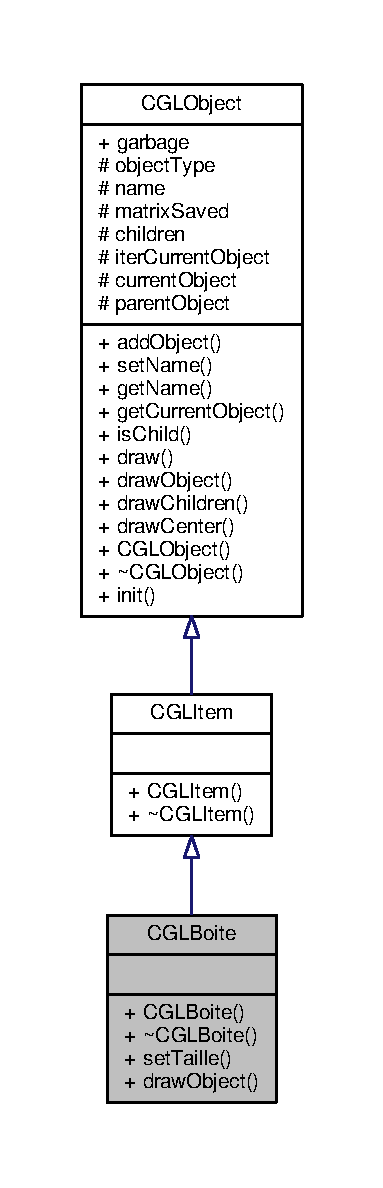
\includegraphics[height=550pt]{d2/d90/class_c_g_l_boite__inherit__graph}
\end{center}
\end{figure}


Graphe de collaboration de C\-G\-L\-Boite\-:\nopagebreak
\begin{figure}[H]
\begin{center}
\leavevmode
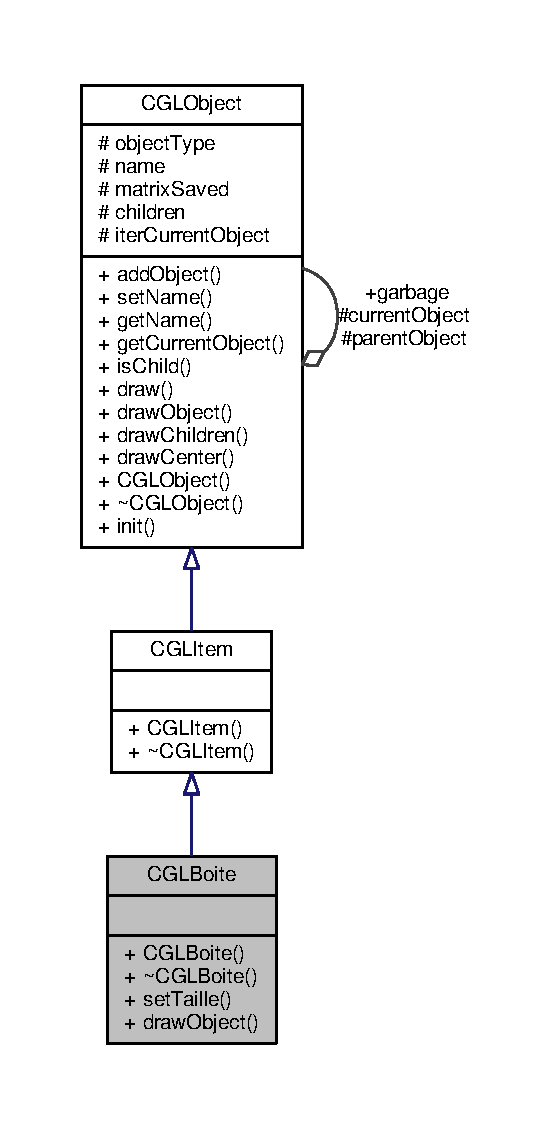
\includegraphics[width=267pt]{db/da1/class_c_g_l_boite__coll__graph}
\end{center}
\end{figure}
\subsection*{Fonctions membres publiques}
\begin{DoxyCompactItemize}
\item 
\hyperlink{class_c_g_l_boite_a9e7f9611e7a265f45bfc93d0c2546a12}{C\-G\-L\-Boite} ()
\item 
virtual \hyperlink{class_c_g_l_boite_a29ac55b7ecc365928a6506a92e709d24}{$\sim$\-C\-G\-L\-Boite} ()
\item 
void \hyperlink{class_c_g_l_boite_aadb5f6701470652fc1232bb36a3fedd8}{set\-Taille} (double, double, double)
\item 
void \hyperlink{class_c_g_l_boite_adc20f63de77be2f8a93500f0065b5e27}{draw\-Object} (Uint32 time\-Ellapsed)
\end{DoxyCompactItemize}
\subsection*{Membres hérités additionnels}


\subsection{Description détaillée}


Définition à la ligne 13 du fichier C\-G\-L\-Boite.\-h.



\subsection{Documentation des constructeurs et destructeur}
\hypertarget{class_c_g_l_boite_a9e7f9611e7a265f45bfc93d0c2546a12}{\index{C\-G\-L\-Boite@{C\-G\-L\-Boite}!C\-G\-L\-Boite@{C\-G\-L\-Boite}}
\index{C\-G\-L\-Boite@{C\-G\-L\-Boite}!CGLBoite@{C\-G\-L\-Boite}}
\subsubsection[{C\-G\-L\-Boite}]{\setlength{\rightskip}{0pt plus 5cm}C\-G\-L\-Boite\-::\-C\-G\-L\-Boite (
\begin{DoxyParamCaption}
{}
\end{DoxyParamCaption}
)}}\label{class_c_g_l_boite_a9e7f9611e7a265f45bfc93d0c2546a12}


Définition à la ligne 10 du fichier C\-G\-L\-Boite.\-cpp.

\hypertarget{class_c_g_l_boite_a29ac55b7ecc365928a6506a92e709d24}{\index{C\-G\-L\-Boite@{C\-G\-L\-Boite}!$\sim$\-C\-G\-L\-Boite@{$\sim$\-C\-G\-L\-Boite}}
\index{$\sim$\-C\-G\-L\-Boite@{$\sim$\-C\-G\-L\-Boite}!CGLBoite@{C\-G\-L\-Boite}}
\subsubsection[{$\sim$\-C\-G\-L\-Boite}]{\setlength{\rightskip}{0pt plus 5cm}C\-G\-L\-Boite\-::$\sim$\-C\-G\-L\-Boite (
\begin{DoxyParamCaption}
{}
\end{DoxyParamCaption}
)\hspace{0.3cm}{\ttfamily [virtual]}}}\label{class_c_g_l_boite_a29ac55b7ecc365928a6506a92e709d24}


Définition à la ligne 16 du fichier C\-G\-L\-Boite.\-cpp.



\subsection{Documentation des fonctions membres}
\hypertarget{class_c_g_l_boite_adc20f63de77be2f8a93500f0065b5e27}{\index{C\-G\-L\-Boite@{C\-G\-L\-Boite}!draw\-Object@{draw\-Object}}
\index{draw\-Object@{draw\-Object}!CGLBoite@{C\-G\-L\-Boite}}
\subsubsection[{draw\-Object}]{\setlength{\rightskip}{0pt plus 5cm}void C\-G\-L\-Boite\-::draw\-Object (
\begin{DoxyParamCaption}
\item[{Uint32}]{time\-Ellapsed}
\end{DoxyParamCaption}
)\hspace{0.3cm}{\ttfamily [virtual]}}}\label{class_c_g_l_boite_adc20f63de77be2f8a93500f0065b5e27}


Réimplémentée à partir de \hyperlink{class_c_g_l_object_a2781ec98c37bd209f2382c5130a365b9}{C\-G\-L\-Object}.



Définition à la ligne 26 du fichier C\-G\-L\-Boite.\-cpp.

\hypertarget{class_c_g_l_boite_aadb5f6701470652fc1232bb36a3fedd8}{\index{C\-G\-L\-Boite@{C\-G\-L\-Boite}!set\-Taille@{set\-Taille}}
\index{set\-Taille@{set\-Taille}!CGLBoite@{C\-G\-L\-Boite}}
\subsubsection[{set\-Taille}]{\setlength{\rightskip}{0pt plus 5cm}void C\-G\-L\-Boite\-::set\-Taille (
\begin{DoxyParamCaption}
\item[{double}]{xv, }
\item[{double}]{yv, }
\item[{double}]{zv}
\end{DoxyParamCaption}
)}}\label{class_c_g_l_boite_aadb5f6701470652fc1232bb36a3fedd8}


Définition à la ligne 19 du fichier C\-G\-L\-Boite.\-cpp.



Voici le graphe des appelants de cette fonction \-:\nopagebreak
\begin{figure}[H]
\begin{center}
\leavevmode
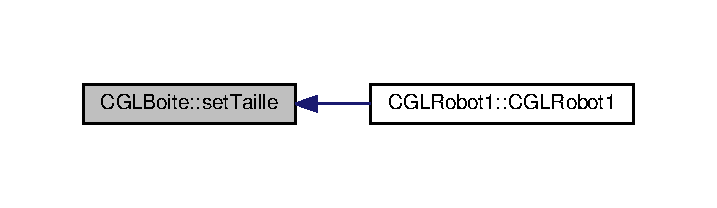
\includegraphics[width=344pt]{dd/daf/class_c_g_l_boite_aadb5f6701470652fc1232bb36a3fedd8_icgraph}
\end{center}
\end{figure}




La documentation de cette classe a été générée à partir des fichiers suivants \-:\begin{DoxyCompactItemize}
\item 
/home/dagal/git/\-Damier\-G\-L/\-Damier\-G\-L/src/\-C\-G\-L/\hyperlink{_c_g_l_boite_8h}{C\-G\-L\-Boite.\-h}\item 
/home/dagal/git/\-Damier\-G\-L/\-Damier\-G\-L/src/\-C\-G\-L/\hyperlink{_c_g_l_boite_8cpp}{C\-G\-L\-Boite.\-cpp}\end{DoxyCompactItemize}

\hypertarget{class_c_g_l_camera}{\section{Référence de la classe C\-G\-L\-Camera}
\label{class_c_g_l_camera}\index{C\-G\-L\-Camera@{C\-G\-L\-Camera}}
}


{\ttfamily \#include $<$C\-G\-L\-Camera.\-h$>$}



Graphe d'héritage de C\-G\-L\-Camera\-:\nopagebreak
\begin{figure}[H]
\begin{center}
\leavevmode
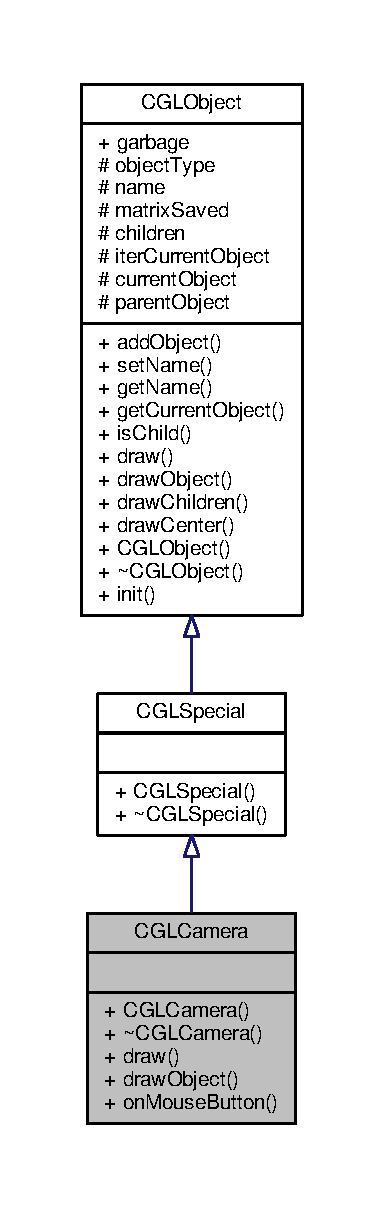
\includegraphics[height=550pt]{d6/d9a/class_c_g_l_camera__inherit__graph}
\end{center}
\end{figure}


Graphe de collaboration de C\-G\-L\-Camera\-:\nopagebreak
\begin{figure}[H]
\begin{center}
\leavevmode
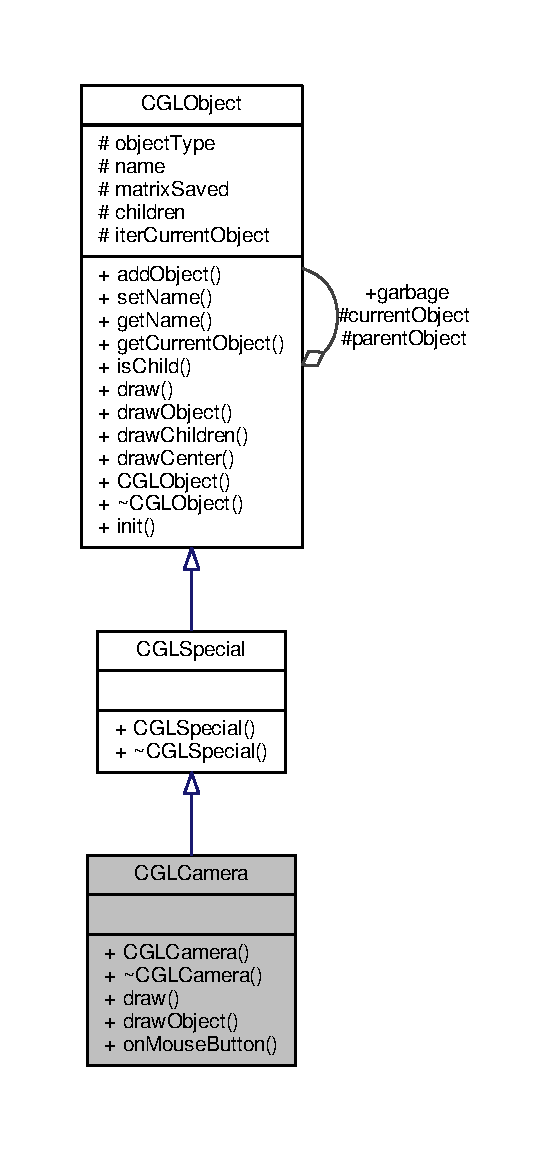
\includegraphics[height=550pt]{d0/d98/class_c_g_l_camera__coll__graph}
\end{center}
\end{figure}
\subsection*{Fonctions membres publiques}
\begin{DoxyCompactItemize}
\item 
\hyperlink{class_c_g_l_camera_a5d3aca0bd9e9f3c7aa1a93474ff63199}{C\-G\-L\-Camera} ()
\item 
virtual \hyperlink{class_c_g_l_camera_adc9a9432202a4f4e3b83bff97c5e4690}{$\sim$\-C\-G\-L\-Camera} ()
\item 
void \hyperlink{class_c_g_l_camera_aba86bb34d99b382e044a52291a3ad435}{draw} (Uint32 time\-Ellapsed)
\item 
void \hyperlink{class_c_g_l_camera_a804d27abd87be682a5b508fe5f0a4451}{draw\-Object} (Uint32 time\-Ellapsed)
\item 
void \hyperlink{class_c_g_l_camera_ad0f4898351c8df558a627102f233ded8}{on\-Mouse\-Button} (S\-D\-L\-\_\-\-Mouse\-Button\-Event \&event)
\end{DoxyCompactItemize}
\subsection*{Membres hérités additionnels}


\subsection{Description détaillée}


Définition à la ligne 13 du fichier C\-G\-L\-Camera.\-h.



\subsection{Documentation des constructeurs et destructeur}
\hypertarget{class_c_g_l_camera_a5d3aca0bd9e9f3c7aa1a93474ff63199}{\index{C\-G\-L\-Camera@{C\-G\-L\-Camera}!C\-G\-L\-Camera@{C\-G\-L\-Camera}}
\index{C\-G\-L\-Camera@{C\-G\-L\-Camera}!CGLCamera@{C\-G\-L\-Camera}}
\subsubsection[{C\-G\-L\-Camera}]{\setlength{\rightskip}{0pt plus 5cm}C\-G\-L\-Camera\-::\-C\-G\-L\-Camera (
\begin{DoxyParamCaption}
{}
\end{DoxyParamCaption}
)}}\label{class_c_g_l_camera_a5d3aca0bd9e9f3c7aa1a93474ff63199}


Définition à la ligne 10 du fichier C\-G\-L\-Camera.\-cpp.

\hypertarget{class_c_g_l_camera_adc9a9432202a4f4e3b83bff97c5e4690}{\index{C\-G\-L\-Camera@{C\-G\-L\-Camera}!$\sim$\-C\-G\-L\-Camera@{$\sim$\-C\-G\-L\-Camera}}
\index{$\sim$\-C\-G\-L\-Camera@{$\sim$\-C\-G\-L\-Camera}!CGLCamera@{C\-G\-L\-Camera}}
\subsubsection[{$\sim$\-C\-G\-L\-Camera}]{\setlength{\rightskip}{0pt plus 5cm}C\-G\-L\-Camera\-::$\sim$\-C\-G\-L\-Camera (
\begin{DoxyParamCaption}
{}
\end{DoxyParamCaption}
)\hspace{0.3cm}{\ttfamily [virtual]}}}\label{class_c_g_l_camera_adc9a9432202a4f4e3b83bff97c5e4690}


Définition à la ligne 25 du fichier C\-G\-L\-Camera.\-cpp.



\subsection{Documentation des fonctions membres}
\hypertarget{class_c_g_l_camera_aba86bb34d99b382e044a52291a3ad435}{\index{C\-G\-L\-Camera@{C\-G\-L\-Camera}!draw@{draw}}
\index{draw@{draw}!CGLCamera@{C\-G\-L\-Camera}}
\subsubsection[{draw}]{\setlength{\rightskip}{0pt plus 5cm}void C\-G\-L\-Camera\-::draw (
\begin{DoxyParamCaption}
\item[{Uint32}]{time\-Ellapsed}
\end{DoxyParamCaption}
)}}\label{class_c_g_l_camera_aba86bb34d99b382e044a52291a3ad435}
\hypertarget{class_c_g_l_camera_a804d27abd87be682a5b508fe5f0a4451}{\index{C\-G\-L\-Camera@{C\-G\-L\-Camera}!draw\-Object@{draw\-Object}}
\index{draw\-Object@{draw\-Object}!CGLCamera@{C\-G\-L\-Camera}}
\subsubsection[{draw\-Object}]{\setlength{\rightskip}{0pt plus 5cm}void C\-G\-L\-Camera\-::draw\-Object (
\begin{DoxyParamCaption}
\item[{Uint32}]{time\-Ellapsed}
\end{DoxyParamCaption}
)\hspace{0.3cm}{\ttfamily [virtual]}}}\label{class_c_g_l_camera_a804d27abd87be682a5b508fe5f0a4451}


Réimplémentée à partir de \hyperlink{class_c_g_l_object_a2781ec98c37bd209f2382c5130a365b9}{C\-G\-L\-Object}.



Définition à la ligne 29 du fichier C\-G\-L\-Camera.\-cpp.

\hypertarget{class_c_g_l_camera_ad0f4898351c8df558a627102f233ded8}{\index{C\-G\-L\-Camera@{C\-G\-L\-Camera}!on\-Mouse\-Button@{on\-Mouse\-Button}}
\index{on\-Mouse\-Button@{on\-Mouse\-Button}!CGLCamera@{C\-G\-L\-Camera}}
\subsubsection[{on\-Mouse\-Button}]{\setlength{\rightskip}{0pt plus 5cm}void C\-G\-L\-Camera\-::on\-Mouse\-Button (
\begin{DoxyParamCaption}
\item[{S\-D\-L\-\_\-\-Mouse\-Button\-Event \&}]{event}
\end{DoxyParamCaption}
)}}\label{class_c_g_l_camera_ad0f4898351c8df558a627102f233ded8}


Définition à la ligne 35 du fichier C\-G\-L\-Camera.\-cpp.



Voici le graphe des appelants de cette fonction \-:\nopagebreak
\begin{figure}[H]
\begin{center}
\leavevmode
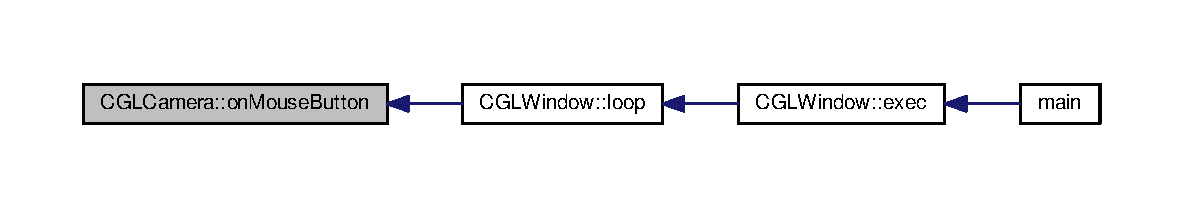
\includegraphics[width=350pt]{de/dee/class_c_g_l_camera_ad0f4898351c8df558a627102f233ded8_icgraph}
\end{center}
\end{figure}




La documentation de cette classe a été générée à partir des fichiers suivants \-:\begin{DoxyCompactItemize}
\item 
/home/dagal/git/\-Damier\-G\-L/\-Damier\-G\-L/src/\-C\-G\-L/\hyperlink{_c_g_l_camera_8h}{C\-G\-L\-Camera.\-h}\item 
/home/dagal/git/\-Damier\-G\-L/\-Damier\-G\-L/src/\-C\-G\-L/\hyperlink{_c_g_l_camera_8cpp}{C\-G\-L\-Camera.\-cpp}\end{DoxyCompactItemize}

\hypertarget{class_c_g_l_camera_list}{\section{Référence de la classe C\-G\-L\-Camera\-List}
\label{class_c_g_l_camera_list}\index{C\-G\-L\-Camera\-List@{C\-G\-L\-Camera\-List}}
}


{\ttfamily \#include $<$C\-G\-L\-Camera\-List.\-h$>$}



Graphe d'héritage de C\-G\-L\-Camera\-List\-:\nopagebreak
\begin{figure}[H]
\begin{center}
\leavevmode
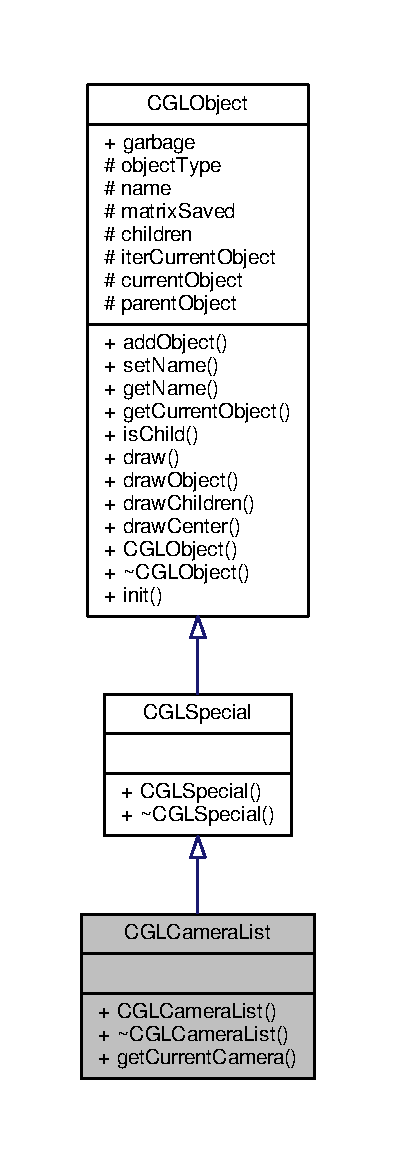
\includegraphics[height=550pt]{dc/dfa/class_c_g_l_camera_list__inherit__graph}
\end{center}
\end{figure}


Graphe de collaboration de C\-G\-L\-Camera\-List\-:\nopagebreak
\begin{figure}[H]
\begin{center}
\leavevmode
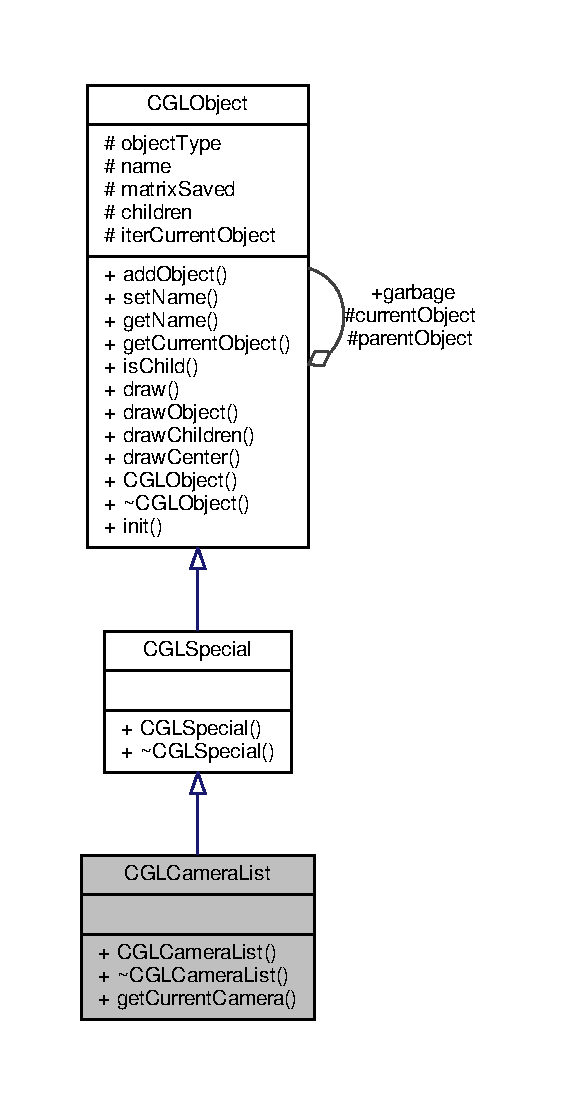
\includegraphics[width=270pt]{d7/ddf/class_c_g_l_camera_list__coll__graph}
\end{center}
\end{figure}
\subsection*{Fonctions membres publiques}
\begin{DoxyCompactItemize}
\item 
\hyperlink{class_c_g_l_camera_list_a97edbfb008863a2dc7781e8f13f90a07}{C\-G\-L\-Camera\-List} ()
\item 
virtual \hyperlink{class_c_g_l_camera_list_a713472acd7976a3e3c0629d594177f7c}{$\sim$\-C\-G\-L\-Camera\-List} ()
\item 
\hyperlink{class_c_g_l_camera}{C\-G\-L\-Camera} $\ast$ \hyperlink{class_c_g_l_camera_list_a9733e24181c1d00620aaece73bc71e5e}{get\-Current\-Camera} ()
\end{DoxyCompactItemize}
\subsection*{Membres hérités additionnels}


\subsection{Description détaillée}


Définition à la ligne 16 du fichier C\-G\-L\-Camera\-List.\-h.



\subsection{Documentation des constructeurs et destructeur}
\hypertarget{class_c_g_l_camera_list_a97edbfb008863a2dc7781e8f13f90a07}{\index{C\-G\-L\-Camera\-List@{C\-G\-L\-Camera\-List}!C\-G\-L\-Camera\-List@{C\-G\-L\-Camera\-List}}
\index{C\-G\-L\-Camera\-List@{C\-G\-L\-Camera\-List}!CGLCameraList@{C\-G\-L\-Camera\-List}}
\subsubsection[{C\-G\-L\-Camera\-List}]{\setlength{\rightskip}{0pt plus 5cm}C\-G\-L\-Camera\-List\-::\-C\-G\-L\-Camera\-List (
\begin{DoxyParamCaption}
{}
\end{DoxyParamCaption}
)}}\label{class_c_g_l_camera_list_a97edbfb008863a2dc7781e8f13f90a07}


Définition à la ligne 10 du fichier C\-G\-L\-Camera\-List.\-cpp.

\hypertarget{class_c_g_l_camera_list_a713472acd7976a3e3c0629d594177f7c}{\index{C\-G\-L\-Camera\-List@{C\-G\-L\-Camera\-List}!$\sim$\-C\-G\-L\-Camera\-List@{$\sim$\-C\-G\-L\-Camera\-List}}
\index{$\sim$\-C\-G\-L\-Camera\-List@{$\sim$\-C\-G\-L\-Camera\-List}!CGLCameraList@{C\-G\-L\-Camera\-List}}
\subsubsection[{$\sim$\-C\-G\-L\-Camera\-List}]{\setlength{\rightskip}{0pt plus 5cm}C\-G\-L\-Camera\-List\-::$\sim$\-C\-G\-L\-Camera\-List (
\begin{DoxyParamCaption}
{}
\end{DoxyParamCaption}
)\hspace{0.3cm}{\ttfamily [virtual]}}}\label{class_c_g_l_camera_list_a713472acd7976a3e3c0629d594177f7c}


Définition à la ligne 14 du fichier C\-G\-L\-Camera\-List.\-cpp.



\subsection{Documentation des fonctions membres}
\hypertarget{class_c_g_l_camera_list_a9733e24181c1d00620aaece73bc71e5e}{\index{C\-G\-L\-Camera\-List@{C\-G\-L\-Camera\-List}!get\-Current\-Camera@{get\-Current\-Camera}}
\index{get\-Current\-Camera@{get\-Current\-Camera}!CGLCameraList@{C\-G\-L\-Camera\-List}}
\subsubsection[{get\-Current\-Camera}]{\setlength{\rightskip}{0pt plus 5cm}{\bf C\-G\-L\-Camera} $\ast$ C\-G\-L\-Camera\-List\-::get\-Current\-Camera (
\begin{DoxyParamCaption}
{}
\end{DoxyParamCaption}
)}}\label{class_c_g_l_camera_list_a9733e24181c1d00620aaece73bc71e5e}


Définition à la ligne 18 du fichier C\-G\-L\-Camera\-List.\-cpp.



La documentation de cette classe a été générée à partir des fichiers suivants \-:\begin{DoxyCompactItemize}
\item 
/home/dagal/git/\-Damier\-G\-L/\-Damier\-G\-L/src/\-C\-G\-L/\hyperlink{_c_g_l_camera_list_8h}{C\-G\-L\-Camera\-List.\-h}\item 
/home/dagal/git/\-Damier\-G\-L/\-Damier\-G\-L/src/\-C\-G\-L/\hyperlink{_c_g_l_camera_list_8cpp}{C\-G\-L\-Camera\-List.\-cpp}\end{DoxyCompactItemize}

\hypertarget{class_c_g_l_circle}{\section{Référence de la classe C\-G\-L\-Circle}
\label{class_c_g_l_circle}\index{C\-G\-L\-Circle@{C\-G\-L\-Circle}}
}


{\ttfamily \#include $<$C\-G\-L\-Circle.\-h$>$}



Graphe d'héritage de C\-G\-L\-Circle\-:\nopagebreak
\begin{figure}[H]
\begin{center}
\leavevmode
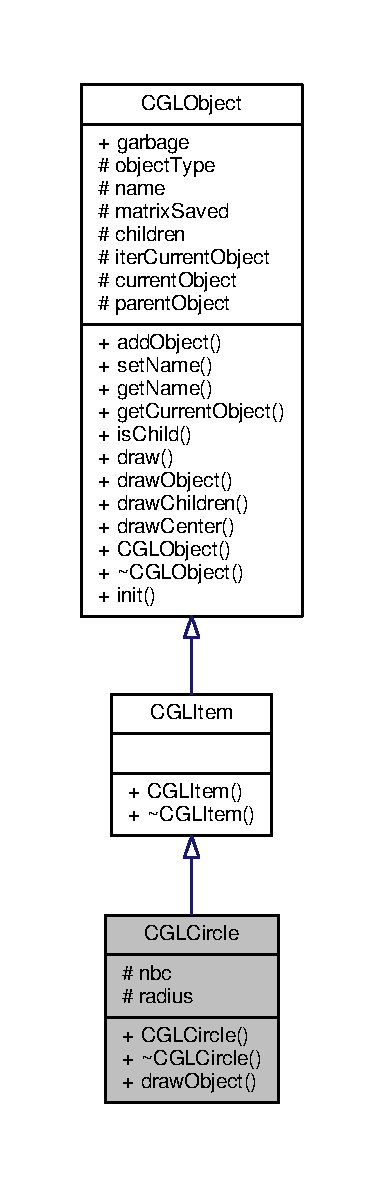
\includegraphics[height=550pt]{df/d3e/class_c_g_l_circle__inherit__graph}
\end{center}
\end{figure}


Graphe de collaboration de C\-G\-L\-Circle\-:\nopagebreak
\begin{figure}[H]
\begin{center}
\leavevmode
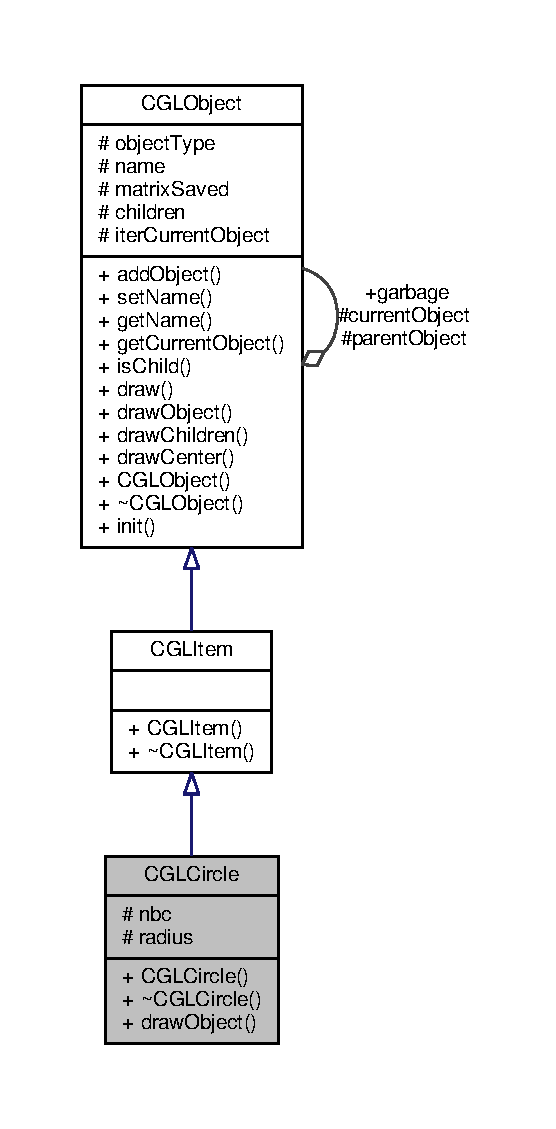
\includegraphics[width=267pt]{d6/dd4/class_c_g_l_circle__coll__graph}
\end{center}
\end{figure}
\subsection*{Fonctions membres publiques}
\begin{DoxyCompactItemize}
\item 
\hyperlink{class_c_g_l_circle_a1fe3551de86200bfe24974c3c525c40a}{C\-G\-L\-Circle} ()
\item 
virtual \hyperlink{class_c_g_l_circle_ab84374a651938aef9342e2eba537f38b}{$\sim$\-C\-G\-L\-Circle} ()
\item 
void \hyperlink{class_c_g_l_circle_a222f67da86a92a075011ec607154b1f8}{draw\-Object} (Uint32 ellapsed\-Time)
\end{DoxyCompactItemize}
\subsection*{Attributs protégés}
\begin{DoxyCompactItemize}
\item 
int \hyperlink{class_c_g_l_circle_a62ec1511c819f9763120183b31461649}{nbc}
\item 
double \hyperlink{class_c_g_l_circle_a6d9f27bacb29deaf5412d5c63d17dca9}{radius}
\end{DoxyCompactItemize}
\subsection*{Membres hérités additionnels}


\subsection{Description détaillée}


Définition à la ligne 19 du fichier C\-G\-L\-Circle.\-h.



\subsection{Documentation des constructeurs et destructeur}
\hypertarget{class_c_g_l_circle_a1fe3551de86200bfe24974c3c525c40a}{\index{C\-G\-L\-Circle@{C\-G\-L\-Circle}!C\-G\-L\-Circle@{C\-G\-L\-Circle}}
\index{C\-G\-L\-Circle@{C\-G\-L\-Circle}!CGLCircle@{C\-G\-L\-Circle}}
\subsubsection[{C\-G\-L\-Circle}]{\setlength{\rightskip}{0pt plus 5cm}C\-G\-L\-Circle\-::\-C\-G\-L\-Circle (
\begin{DoxyParamCaption}
{}
\end{DoxyParamCaption}
)}}\label{class_c_g_l_circle_a1fe3551de86200bfe24974c3c525c40a}


Définition à la ligne 10 du fichier C\-G\-L\-Circle.\-cpp.

\hypertarget{class_c_g_l_circle_ab84374a651938aef9342e2eba537f38b}{\index{C\-G\-L\-Circle@{C\-G\-L\-Circle}!$\sim$\-C\-G\-L\-Circle@{$\sim$\-C\-G\-L\-Circle}}
\index{$\sim$\-C\-G\-L\-Circle@{$\sim$\-C\-G\-L\-Circle}!CGLCircle@{C\-G\-L\-Circle}}
\subsubsection[{$\sim$\-C\-G\-L\-Circle}]{\setlength{\rightskip}{0pt plus 5cm}C\-G\-L\-Circle\-::$\sim$\-C\-G\-L\-Circle (
\begin{DoxyParamCaption}
{}
\end{DoxyParamCaption}
)\hspace{0.3cm}{\ttfamily [virtual]}}}\label{class_c_g_l_circle_ab84374a651938aef9342e2eba537f38b}


Définition à la ligne 14 du fichier C\-G\-L\-Circle.\-cpp.



\subsection{Documentation des fonctions membres}
\hypertarget{class_c_g_l_circle_a222f67da86a92a075011ec607154b1f8}{\index{C\-G\-L\-Circle@{C\-G\-L\-Circle}!draw\-Object@{draw\-Object}}
\index{draw\-Object@{draw\-Object}!CGLCircle@{C\-G\-L\-Circle}}
\subsubsection[{draw\-Object}]{\setlength{\rightskip}{0pt plus 5cm}void C\-G\-L\-Circle\-::draw\-Object (
\begin{DoxyParamCaption}
\item[{Uint32}]{ellapsed\-Time}
\end{DoxyParamCaption}
)\hspace{0.3cm}{\ttfamily [virtual]}}}\label{class_c_g_l_circle_a222f67da86a92a075011ec607154b1f8}


Réimplémentée à partir de \hyperlink{class_c_g_l_object_a2781ec98c37bd209f2382c5130a365b9}{C\-G\-L\-Object}.



Définition à la ligne 18 du fichier C\-G\-L\-Circle.\-cpp.



\subsection{Documentation des données membres}
\hypertarget{class_c_g_l_circle_a62ec1511c819f9763120183b31461649}{\index{C\-G\-L\-Circle@{C\-G\-L\-Circle}!nbc@{nbc}}
\index{nbc@{nbc}!CGLCircle@{C\-G\-L\-Circle}}
\subsubsection[{nbc}]{\setlength{\rightskip}{0pt plus 5cm}int C\-G\-L\-Circle\-::nbc\hspace{0.3cm}{\ttfamily [protected]}}}\label{class_c_g_l_circle_a62ec1511c819f9763120183b31461649}


Définition à la ligne 22 du fichier C\-G\-L\-Circle.\-h.

\hypertarget{class_c_g_l_circle_a6d9f27bacb29deaf5412d5c63d17dca9}{\index{C\-G\-L\-Circle@{C\-G\-L\-Circle}!radius@{radius}}
\index{radius@{radius}!CGLCircle@{C\-G\-L\-Circle}}
\subsubsection[{radius}]{\setlength{\rightskip}{0pt plus 5cm}double C\-G\-L\-Circle\-::radius\hspace{0.3cm}{\ttfamily [protected]}}}\label{class_c_g_l_circle_a6d9f27bacb29deaf5412d5c63d17dca9}


Définition à la ligne 23 du fichier C\-G\-L\-Circle.\-h.



La documentation de cette classe a été générée à partir des fichiers suivants \-:\begin{DoxyCompactItemize}
\item 
/home/dagal/git/\-Damier\-G\-L/\-Damier\-G\-L/src/\-C\-G\-L/\hyperlink{_c_g_l_circle_8h}{C\-G\-L\-Circle.\-h}\item 
/home/dagal/git/\-Damier\-G\-L/\-Damier\-G\-L/src/\-C\-G\-L/\hyperlink{_c_g_l_circle_8cpp}{C\-G\-L\-Circle.\-cpp}\end{DoxyCompactItemize}

\hypertarget{class_c_g_l_color}{\section{Référence de la classe C\-G\-L\-Color}
\label{class_c_g_l_color}\index{C\-G\-L\-Color@{C\-G\-L\-Color}}
}


{\ttfamily \#include $<$C\-G\-L\-Color.\-h$>$}



Graphe d'héritage de C\-G\-L\-Color\-:
\nopagebreak
\begin{figure}[H]
\begin{center}
\leavevmode
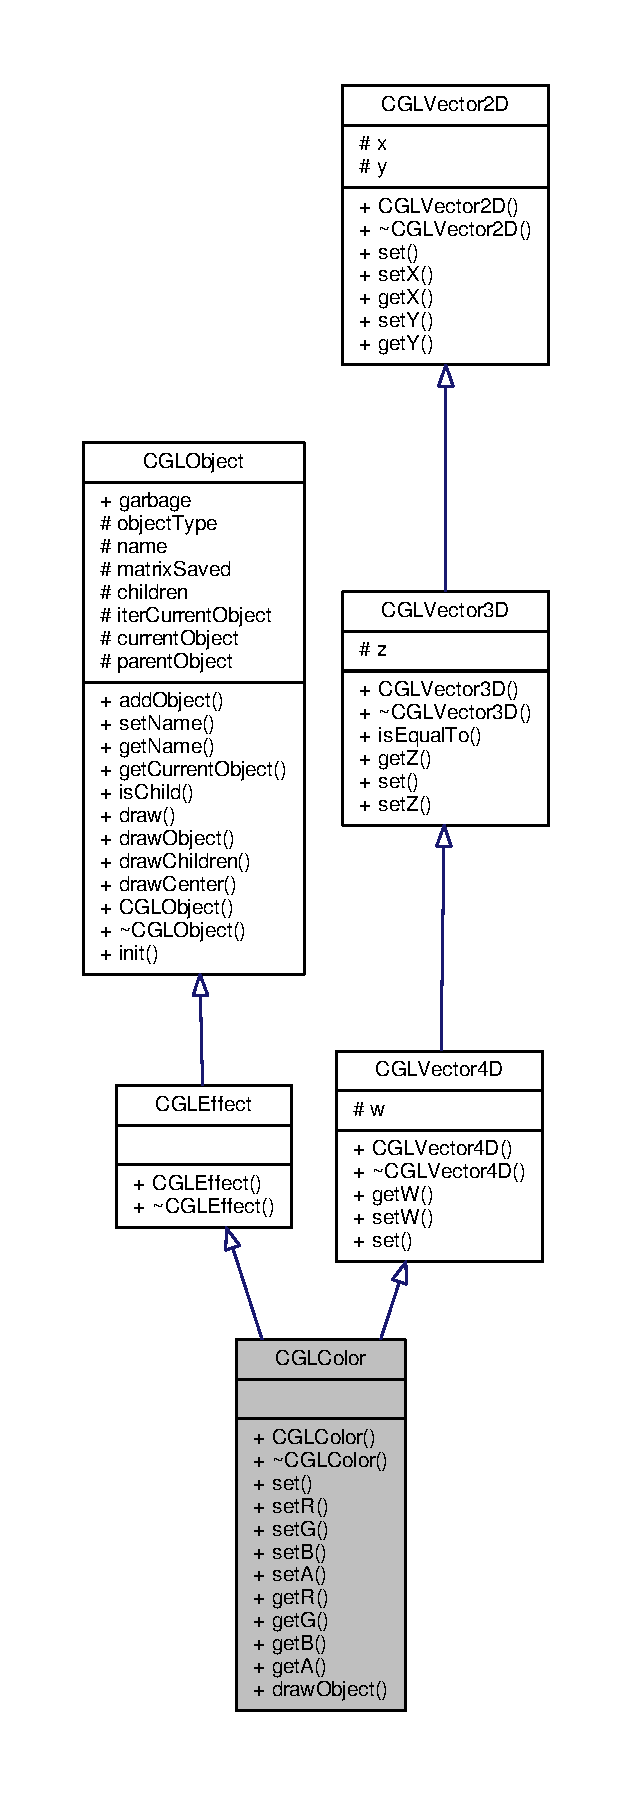
\includegraphics[height=550pt]{d0/d0d/class_c_g_l_color__inherit__graph}
\end{center}
\end{figure}


Graphe de collaboration de C\-G\-L\-Color\-:
\nopagebreak
\begin{figure}[H]
\begin{center}
\leavevmode
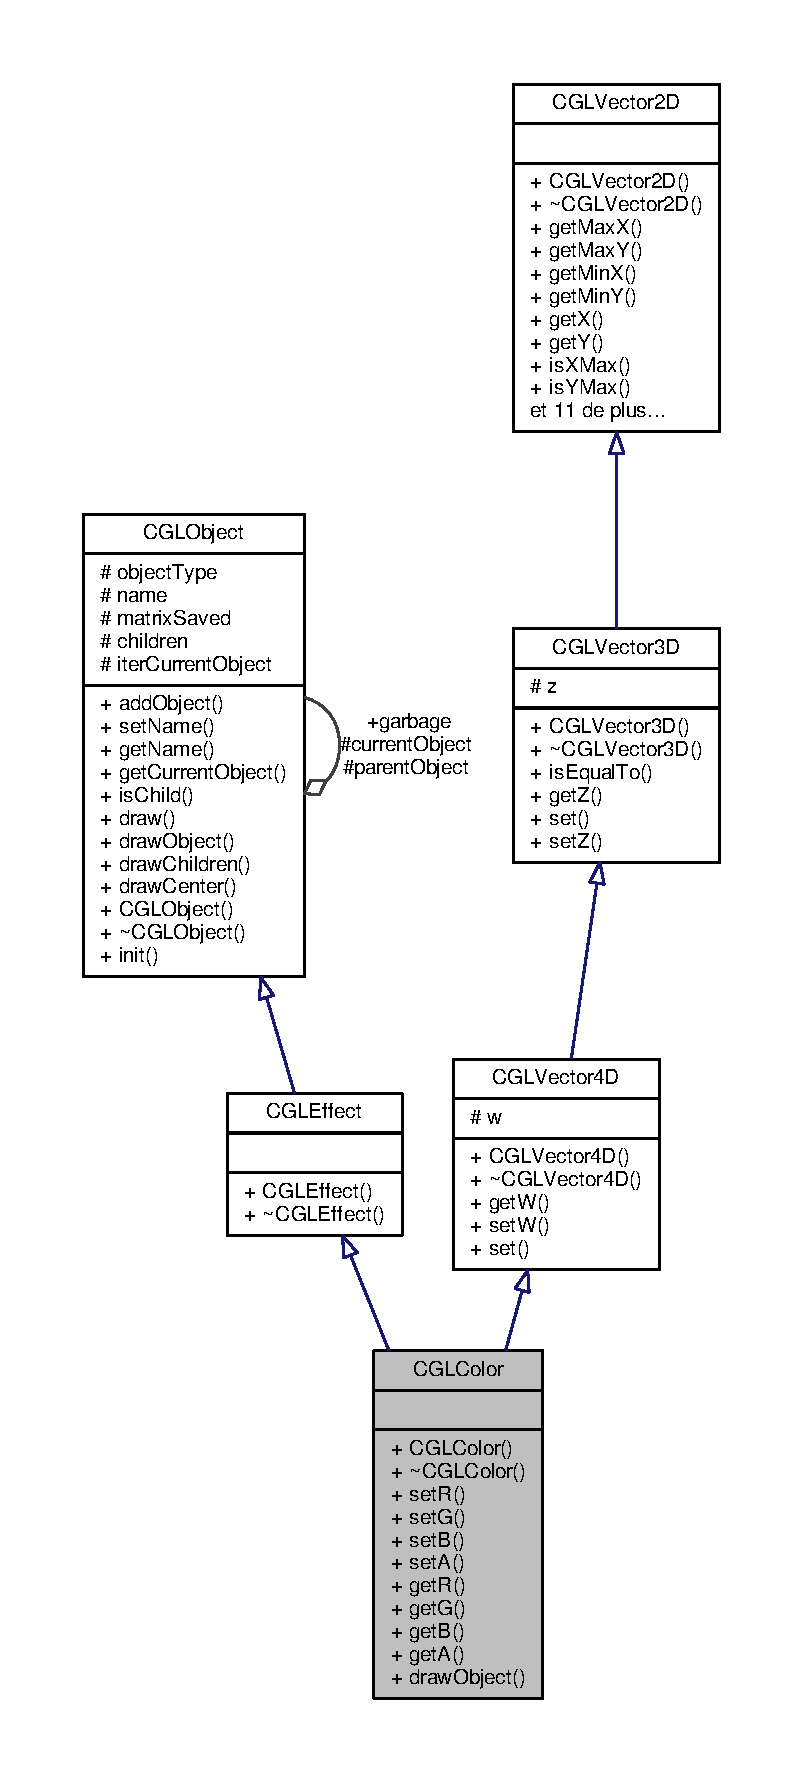
\includegraphics[height=550pt]{d0/d7c/class_c_g_l_color__coll__graph}
\end{center}
\end{figure}
\subsection*{Fonctions membres publiques}
\begin{DoxyCompactItemize}
\item 
\hyperlink{class_c_g_l_color_ab6e65b639ac6545e43d3b54ef9de7eaf}{C\-G\-L\-Color} ()
\item 
virtual \hyperlink{class_c_g_l_color_ad5d7a52bc05be0c30b50a1c3bc64bbd6}{$\sim$\-C\-G\-L\-Color} ()
\item 
void \hyperlink{class_c_g_l_color_af025a76284d339268246c03a929f27f4}{set\-R} (double rv)
\item 
void \hyperlink{class_c_g_l_color_a2b737fc4b94021e2cdaad2c1c98d3cef}{set\-G} (double gv)
\item 
void \hyperlink{class_c_g_l_color_ac898e4d49846a3b3788daeb535c5bccc}{set\-B} (double bv)
\item 
void \hyperlink{class_c_g_l_color_a4bf56920a8621fcc8db155b7cc60d5a1}{set\-A} (double av)
\item 
double \hyperlink{class_c_g_l_color_ac6d5a5366ee03d2061d6c79981d322c4}{get\-R} ()
\item 
double \hyperlink{class_c_g_l_color_a49f6584fa824f5a08f403d86d0bdfcf0}{get\-G} ()
\item 
double \hyperlink{class_c_g_l_color_a2908eed3bfda5ae231dbafd8df81daec}{get\-B} ()
\item 
double \hyperlink{class_c_g_l_color_a8fd36d7e2f7e55ba24dd95a66ab51c32}{get\-A} ()
\item 
void \hyperlink{class_c_g_l_color_a69d92c401c12b7846c458c41a564b3ae}{draw\-Object} (Uint32 time\-Ellapsed)
\end{DoxyCompactItemize}
\subsection*{Membres hérités additionnels}


\subsection{Description détaillée}


Définition à la ligne 17 du fichier C\-G\-L\-Color.\-h.



\subsection{Documentation des constructeurs et destructeur}
\hypertarget{class_c_g_l_color_ab6e65b639ac6545e43d3b54ef9de7eaf}{\index{C\-G\-L\-Color@{C\-G\-L\-Color}!C\-G\-L\-Color@{C\-G\-L\-Color}}
\index{C\-G\-L\-Color@{C\-G\-L\-Color}!CGLColor@{C\-G\-L\-Color}}
\subsubsection[{C\-G\-L\-Color}]{\setlength{\rightskip}{0pt plus 5cm}C\-G\-L\-Color\-::\-C\-G\-L\-Color (
\begin{DoxyParamCaption}
{}
\end{DoxyParamCaption}
)}}\label{class_c_g_l_color_ab6e65b639ac6545e43d3b54ef9de7eaf}


Définition à la ligne 13 du fichier C\-G\-L\-Color.\-cpp.

\hypertarget{class_c_g_l_color_ad5d7a52bc05be0c30b50a1c3bc64bbd6}{\index{C\-G\-L\-Color@{C\-G\-L\-Color}!$\sim$\-C\-G\-L\-Color@{$\sim$\-C\-G\-L\-Color}}
\index{$\sim$\-C\-G\-L\-Color@{$\sim$\-C\-G\-L\-Color}!CGLColor@{C\-G\-L\-Color}}
\subsubsection[{$\sim$\-C\-G\-L\-Color}]{\setlength{\rightskip}{0pt plus 5cm}C\-G\-L\-Color\-::$\sim$\-C\-G\-L\-Color (
\begin{DoxyParamCaption}
{}
\end{DoxyParamCaption}
)\hspace{0.3cm}{\ttfamily [virtual]}}}\label{class_c_g_l_color_ad5d7a52bc05be0c30b50a1c3bc64bbd6}


Définition à la ligne 17 du fichier C\-G\-L\-Color.\-cpp.



\subsection{Documentation des fonctions membres}
\hypertarget{class_c_g_l_color_a69d92c401c12b7846c458c41a564b3ae}{\index{C\-G\-L\-Color@{C\-G\-L\-Color}!draw\-Object@{draw\-Object}}
\index{draw\-Object@{draw\-Object}!CGLColor@{C\-G\-L\-Color}}
\subsubsection[{draw\-Object}]{\setlength{\rightskip}{0pt plus 5cm}void C\-G\-L\-Color\-::draw\-Object (
\begin{DoxyParamCaption}
\item[{Uint32}]{time\-Ellapsed}
\end{DoxyParamCaption}
)\hspace{0.3cm}{\ttfamily [virtual]}}}\label{class_c_g_l_color_a69d92c401c12b7846c458c41a564b3ae}


Réimplémentée à partir de \hyperlink{class_c_g_l_object_a2781ec98c37bd209f2382c5130a365b9}{C\-G\-L\-Object}.



Définition à la ligne 65 du fichier C\-G\-L\-Color.\-cpp.



Voici le graphe d'appel pour cette fonction \-:
\nopagebreak
\begin{figure}[H]
\begin{center}
\leavevmode
\includegraphics[width=340pt]{d7/dd6/class_c_g_l_color_a69d92c401c12b7846c458c41a564b3ae_cgraph}
\end{center}
\end{figure}


\hypertarget{class_c_g_l_color_a8fd36d7e2f7e55ba24dd95a66ab51c32}{\index{C\-G\-L\-Color@{C\-G\-L\-Color}!get\-A@{get\-A}}
\index{get\-A@{get\-A}!CGLColor@{C\-G\-L\-Color}}
\subsubsection[{get\-A}]{\setlength{\rightskip}{0pt plus 5cm}double C\-G\-L\-Color\-::get\-A (
\begin{DoxyParamCaption}
{}
\end{DoxyParamCaption}
)}}\label{class_c_g_l_color_a8fd36d7e2f7e55ba24dd95a66ab51c32}


Définition à la ligne 59 du fichier C\-G\-L\-Color.\-cpp.



Voici le graphe d'appel pour cette fonction \-:
\nopagebreak
\begin{figure}[H]
\begin{center}
\leavevmode
\includegraphics[width=310pt]{d7/dd6/class_c_g_l_color_a8fd36d7e2f7e55ba24dd95a66ab51c32_cgraph}
\end{center}
\end{figure}


\hypertarget{class_c_g_l_color_a2908eed3bfda5ae231dbafd8df81daec}{\index{C\-G\-L\-Color@{C\-G\-L\-Color}!get\-B@{get\-B}}
\index{get\-B@{get\-B}!CGLColor@{C\-G\-L\-Color}}
\subsubsection[{get\-B}]{\setlength{\rightskip}{0pt plus 5cm}double C\-G\-L\-Color\-::get\-B (
\begin{DoxyParamCaption}
{}
\end{DoxyParamCaption}
)}}\label{class_c_g_l_color_a2908eed3bfda5ae231dbafd8df81daec}


Définition à la ligne 53 du fichier C\-G\-L\-Color.\-cpp.



Voici le graphe d'appel pour cette fonction \-:
\nopagebreak
\begin{figure}[H]
\begin{center}
\leavevmode
\includegraphics[width=306pt]{d7/dd6/class_c_g_l_color_a2908eed3bfda5ae231dbafd8df81daec_cgraph}
\end{center}
\end{figure}


\hypertarget{class_c_g_l_color_a49f6584fa824f5a08f403d86d0bdfcf0}{\index{C\-G\-L\-Color@{C\-G\-L\-Color}!get\-G@{get\-G}}
\index{get\-G@{get\-G}!CGLColor@{C\-G\-L\-Color}}
\subsubsection[{get\-G}]{\setlength{\rightskip}{0pt plus 5cm}double C\-G\-L\-Color\-::get\-G (
\begin{DoxyParamCaption}
{}
\end{DoxyParamCaption}
)}}\label{class_c_g_l_color_a49f6584fa824f5a08f403d86d0bdfcf0}


Définition à la ligne 47 du fichier C\-G\-L\-Color.\-cpp.



Voici le graphe d'appel pour cette fonction \-:
\nopagebreak
\begin{figure}[H]
\begin{center}
\leavevmode
\includegraphics[width=308pt]{d7/dd6/class_c_g_l_color_a49f6584fa824f5a08f403d86d0bdfcf0_cgraph}
\end{center}
\end{figure}


\hypertarget{class_c_g_l_color_ac6d5a5366ee03d2061d6c79981d322c4}{\index{C\-G\-L\-Color@{C\-G\-L\-Color}!get\-R@{get\-R}}
\index{get\-R@{get\-R}!CGLColor@{C\-G\-L\-Color}}
\subsubsection[{get\-R}]{\setlength{\rightskip}{0pt plus 5cm}double C\-G\-L\-Color\-::get\-R (
\begin{DoxyParamCaption}
{}
\end{DoxyParamCaption}
)}}\label{class_c_g_l_color_ac6d5a5366ee03d2061d6c79981d322c4}


Définition à la ligne 41 du fichier C\-G\-L\-Color.\-cpp.



Voici le graphe d'appel pour cette fonction \-:
\nopagebreak
\begin{figure}[H]
\begin{center}
\leavevmode
\includegraphics[width=308pt]{d7/dd6/class_c_g_l_color_ac6d5a5366ee03d2061d6c79981d322c4_cgraph}
\end{center}
\end{figure}


\hypertarget{class_c_g_l_color_a4bf56920a8621fcc8db155b7cc60d5a1}{\index{C\-G\-L\-Color@{C\-G\-L\-Color}!set\-A@{set\-A}}
\index{set\-A@{set\-A}!CGLColor@{C\-G\-L\-Color}}
\subsubsection[{set\-A}]{\setlength{\rightskip}{0pt plus 5cm}void C\-G\-L\-Color\-::set\-A (
\begin{DoxyParamCaption}
\item[{double}]{av}
\end{DoxyParamCaption}
)}}\label{class_c_g_l_color_a4bf56920a8621fcc8db155b7cc60d5a1}


Définition à la ligne 36 du fichier C\-G\-L\-Color.\-cpp.



Voici le graphe d'appel pour cette fonction \-:
\nopagebreak
\begin{figure}[H]
\begin{center}
\leavevmode
\includegraphics[width=310pt]{d7/dd6/class_c_g_l_color_a4bf56920a8621fcc8db155b7cc60d5a1_cgraph}
\end{center}
\end{figure}


\hypertarget{class_c_g_l_color_ac898e4d49846a3b3788daeb535c5bccc}{\index{C\-G\-L\-Color@{C\-G\-L\-Color}!set\-B@{set\-B}}
\index{set\-B@{set\-B}!CGLColor@{C\-G\-L\-Color}}
\subsubsection[{set\-B}]{\setlength{\rightskip}{0pt plus 5cm}void C\-G\-L\-Color\-::set\-B (
\begin{DoxyParamCaption}
\item[{double}]{bv}
\end{DoxyParamCaption}
)}}\label{class_c_g_l_color_ac898e4d49846a3b3788daeb535c5bccc}


Définition à la ligne 31 du fichier C\-G\-L\-Color.\-cpp.



Voici le graphe d'appel pour cette fonction \-:
\nopagebreak
\begin{figure}[H]
\begin{center}
\leavevmode
\includegraphics[width=306pt]{d7/dd6/class_c_g_l_color_ac898e4d49846a3b3788daeb535c5bccc_cgraph}
\end{center}
\end{figure}


\hypertarget{class_c_g_l_color_a2b737fc4b94021e2cdaad2c1c98d3cef}{\index{C\-G\-L\-Color@{C\-G\-L\-Color}!set\-G@{set\-G}}
\index{set\-G@{set\-G}!CGLColor@{C\-G\-L\-Color}}
\subsubsection[{set\-G}]{\setlength{\rightskip}{0pt plus 5cm}void C\-G\-L\-Color\-::set\-G (
\begin{DoxyParamCaption}
\item[{double}]{gv}
\end{DoxyParamCaption}
)}}\label{class_c_g_l_color_a2b737fc4b94021e2cdaad2c1c98d3cef}


Définition à la ligne 26 du fichier C\-G\-L\-Color.\-cpp.



Voici le graphe d'appel pour cette fonction \-:
\nopagebreak
\begin{figure}[H]
\begin{center}
\leavevmode
\includegraphics[width=308pt]{d7/dd6/class_c_g_l_color_a2b737fc4b94021e2cdaad2c1c98d3cef_cgraph}
\end{center}
\end{figure}


\hypertarget{class_c_g_l_color_af025a76284d339268246c03a929f27f4}{\index{C\-G\-L\-Color@{C\-G\-L\-Color}!set\-R@{set\-R}}
\index{set\-R@{set\-R}!CGLColor@{C\-G\-L\-Color}}
\subsubsection[{set\-R}]{\setlength{\rightskip}{0pt plus 5cm}void C\-G\-L\-Color\-::set\-R (
\begin{DoxyParamCaption}
\item[{double}]{rv}
\end{DoxyParamCaption}
)}}\label{class_c_g_l_color_af025a76284d339268246c03a929f27f4}


Définition à la ligne 21 du fichier C\-G\-L\-Color.\-cpp.



Voici le graphe d'appel pour cette fonction \-:
\nopagebreak
\begin{figure}[H]
\begin{center}
\leavevmode
\includegraphics[width=308pt]{d7/dd6/class_c_g_l_color_af025a76284d339268246c03a929f27f4_cgraph}
\end{center}
\end{figure}




La documentation de cette classe a été générée à partir des fichiers suivants \-:\begin{DoxyCompactItemize}
\item 
/home/dagal/git/\-Damier\-G\-L/\-Damier\-G\-L/src/\-C\-G\-L/\hyperlink{_c_g_l_color_8h}{C\-G\-L\-Color.\-h}\item 
/home/dagal/git/\-Damier\-G\-L/\-Damier\-G\-L/src/\-C\-G\-L/\hyperlink{_c_g_l_color_8cpp}{C\-G\-L\-Color.\-cpp}\end{DoxyCompactItemize}

\hypertarget{class_c_g_l_dot}{\section{Référence de la classe C\-G\-L\-Dot}
\label{class_c_g_l_dot}\index{C\-G\-L\-Dot@{C\-G\-L\-Dot}}
}


{\ttfamily \#include $<$Dot.\-h$>$}



Graphe d'héritage de C\-G\-L\-Dot\-:
\nopagebreak
\begin{figure}[H]
\begin{center}
\leavevmode
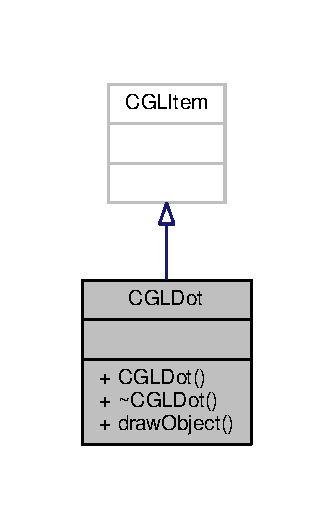
\includegraphics[width=160pt]{d3/d95/class_c_g_l_dot__inherit__graph}
\end{center}
\end{figure}


Graphe de collaboration de C\-G\-L\-Dot\-:
\nopagebreak
\begin{figure}[H]
\begin{center}
\leavevmode
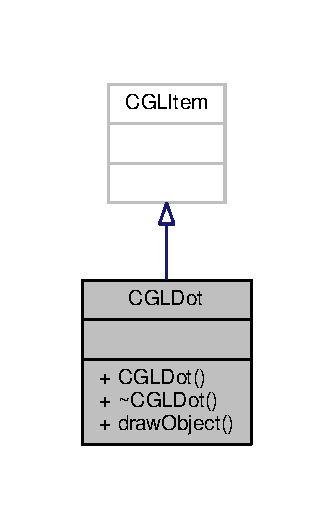
\includegraphics[width=160pt]{d7/d23/class_c_g_l_dot__coll__graph}
\end{center}
\end{figure}
\subsection*{Fonctions membres publiques}
\begin{DoxyCompactItemize}
\item 
\hyperlink{class_c_g_l_dot_a2199cd6c78e18219c88bf707201b003c}{C\-G\-L\-Dot} ()
\item 
virtual \hyperlink{class_c_g_l_dot_a9874d2a0168a7d8489c1bb7a6d6dc02c}{$\sim$\-C\-G\-L\-Dot} ()
\item 
void \hyperlink{class_c_g_l_dot_aba6d02d4c9da30aea263599e66e5f201}{draw\-Object} (Uint32 ellapsed\-Time)
\end{DoxyCompactItemize}


\subsection{Description détaillée}


Définition à la ligne 16 du fichier Dot.\-h.



\subsection{Documentation des constructeurs et destructeur}
\hypertarget{class_c_g_l_dot_a2199cd6c78e18219c88bf707201b003c}{\index{C\-G\-L\-Dot@{C\-G\-L\-Dot}!C\-G\-L\-Dot@{C\-G\-L\-Dot}}
\index{C\-G\-L\-Dot@{C\-G\-L\-Dot}!CGLDot@{C\-G\-L\-Dot}}
\subsubsection[{C\-G\-L\-Dot}]{\setlength{\rightskip}{0pt plus 5cm}C\-G\-L\-Dot\-::\-C\-G\-L\-Dot (
\begin{DoxyParamCaption}
{}
\end{DoxyParamCaption}
)}}\label{class_c_g_l_dot_a2199cd6c78e18219c88bf707201b003c}


Définition à la ligne 10 du fichier Dot.\-cpp.

\hypertarget{class_c_g_l_dot_a9874d2a0168a7d8489c1bb7a6d6dc02c}{\index{C\-G\-L\-Dot@{C\-G\-L\-Dot}!$\sim$\-C\-G\-L\-Dot@{$\sim$\-C\-G\-L\-Dot}}
\index{$\sim$\-C\-G\-L\-Dot@{$\sim$\-C\-G\-L\-Dot}!CGLDot@{C\-G\-L\-Dot}}
\subsubsection[{$\sim$\-C\-G\-L\-Dot}]{\setlength{\rightskip}{0pt plus 5cm}C\-G\-L\-Dot\-::$\sim$\-C\-G\-L\-Dot (
\begin{DoxyParamCaption}
{}
\end{DoxyParamCaption}
)\hspace{0.3cm}{\ttfamily [virtual]}}}\label{class_c_g_l_dot_a9874d2a0168a7d8489c1bb7a6d6dc02c}


Définition à la ligne 14 du fichier Dot.\-cpp.



\subsection{Documentation des fonctions membres}
\hypertarget{class_c_g_l_dot_aba6d02d4c9da30aea263599e66e5f201}{\index{C\-G\-L\-Dot@{C\-G\-L\-Dot}!draw\-Object@{draw\-Object}}
\index{draw\-Object@{draw\-Object}!CGLDot@{C\-G\-L\-Dot}}
\subsubsection[{draw\-Object}]{\setlength{\rightskip}{0pt plus 5cm}void C\-G\-L\-Dot\-::draw\-Object (
\begin{DoxyParamCaption}
\item[{Uint32}]{ellapsed\-Time}
\end{DoxyParamCaption}
)}}\label{class_c_g_l_dot_aba6d02d4c9da30aea263599e66e5f201}


Définition à la ligne 18 du fichier Dot.\-cpp.



La documentation de cette classe a été générée à partir des fichiers suivants \-:\begin{DoxyCompactItemize}
\item 
/home/dagal/git/\-D\-G\-L/\-Damier\-G\-L/src/\-C\-G\-L/\hyperlink{_dot_8h}{Dot.\-h}\item 
/home/dagal/git/\-D\-G\-L/\-Damier\-G\-L/src/\-C\-G\-L/\hyperlink{_dot_8cpp}{Dot.\-cpp}\end{DoxyCompactItemize}

\hypertarget{class_c_g_l_effect}{\section{Référence de la classe C\-G\-L\-Effect}
\label{class_c_g_l_effect}\index{C\-G\-L\-Effect@{C\-G\-L\-Effect}}
}


{\ttfamily \#include $<$C\-G\-L\-Effect.\-h$>$}



Graphe d'héritage de C\-G\-L\-Effect\-:
\nopagebreak
\begin{figure}[H]
\begin{center}
\leavevmode
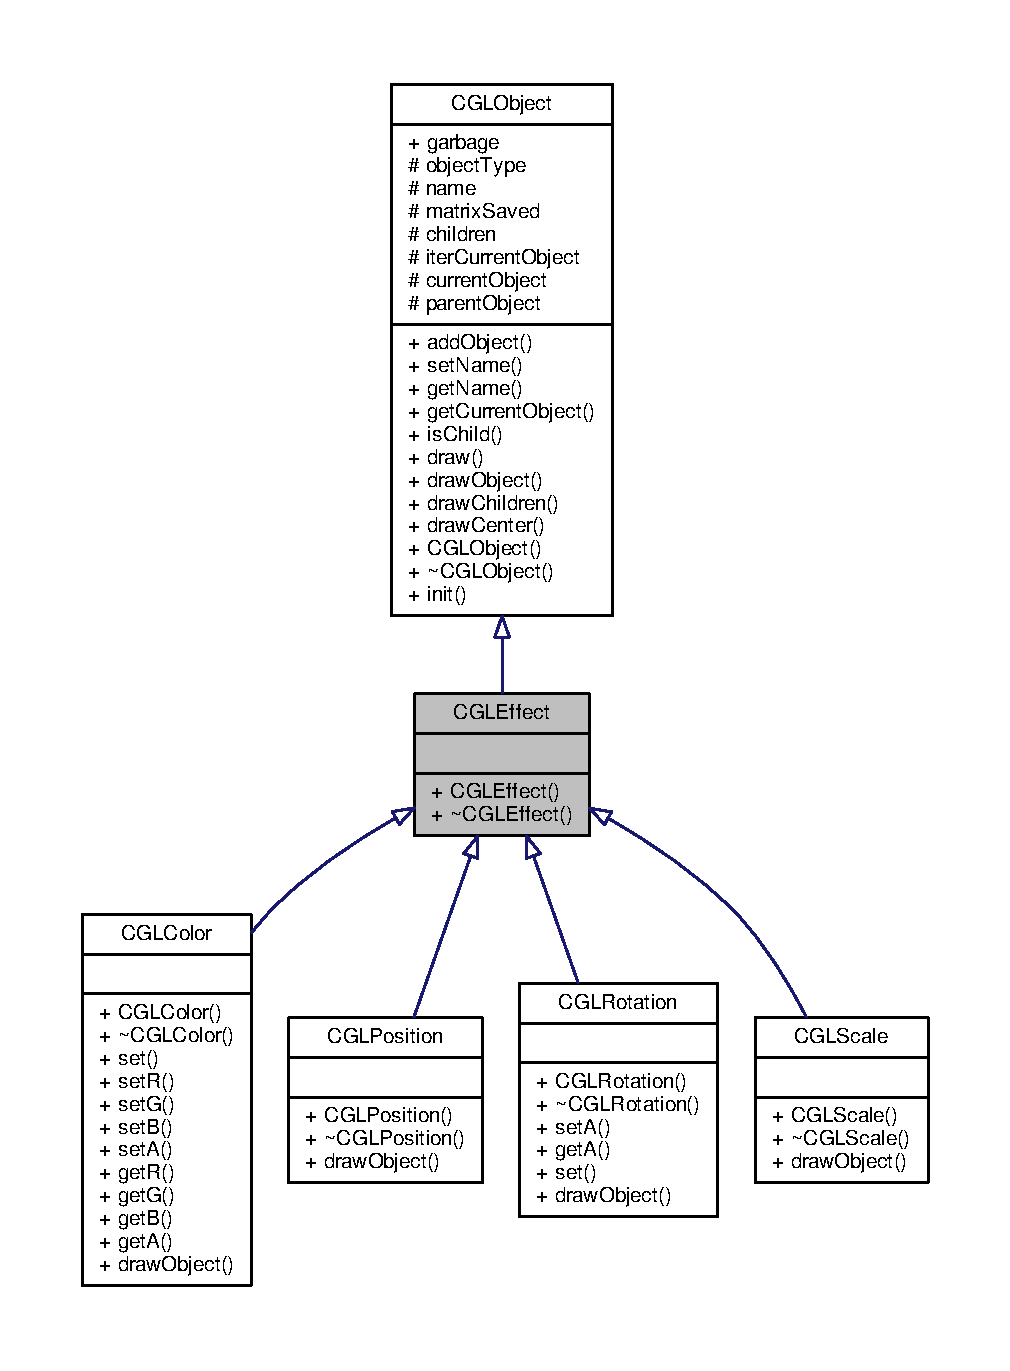
\includegraphics[height=550pt]{d7/d88/class_c_g_l_effect__inherit__graph}
\end{center}
\end{figure}


Graphe de collaboration de C\-G\-L\-Effect\-:\nopagebreak
\begin{figure}[H]
\begin{center}
\leavevmode
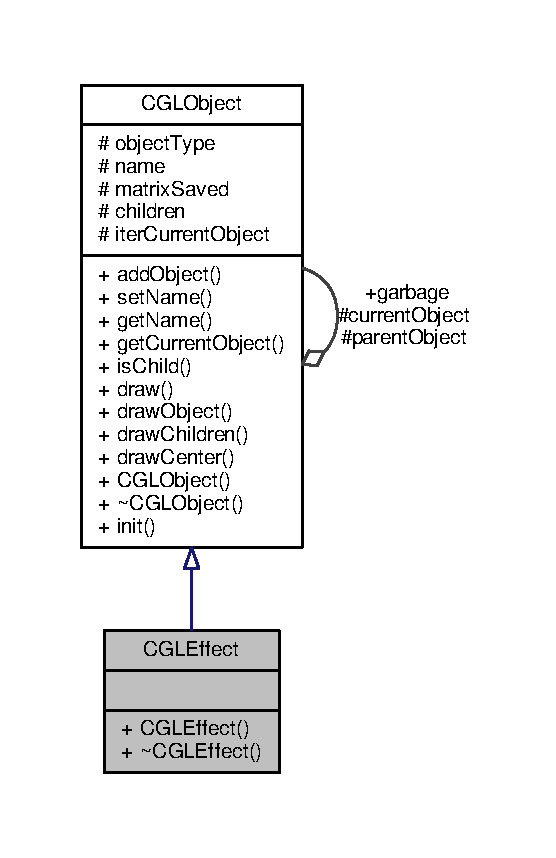
\includegraphics[width=267pt]{d2/d69/class_c_g_l_effect__coll__graph}
\end{center}
\end{figure}
\subsection*{Fonctions membres publiques}
\begin{DoxyCompactItemize}
\item 
\hyperlink{class_c_g_l_effect_ad84b35aafce8ab422f939e5e51d5dd61}{C\-G\-L\-Effect} ()
\item 
virtual \hyperlink{class_c_g_l_effect_ab4bd0b2135fe6b04ed448a2acb0df4cc}{$\sim$\-C\-G\-L\-Effect} ()
\end{DoxyCompactItemize}
\subsection*{Membres hérités additionnels}


\subsection{Description détaillée}


Définition à la ligne 16 du fichier C\-G\-L\-Effect.\-h.



\subsection{Documentation des constructeurs et destructeur}
\hypertarget{class_c_g_l_effect_ad84b35aafce8ab422f939e5e51d5dd61}{\index{C\-G\-L\-Effect@{C\-G\-L\-Effect}!C\-G\-L\-Effect@{C\-G\-L\-Effect}}
\index{C\-G\-L\-Effect@{C\-G\-L\-Effect}!CGLEffect@{C\-G\-L\-Effect}}
\subsubsection[{C\-G\-L\-Effect}]{\setlength{\rightskip}{0pt plus 5cm}C\-G\-L\-Effect\-::\-C\-G\-L\-Effect (
\begin{DoxyParamCaption}
{}
\end{DoxyParamCaption}
)}}\label{class_c_g_l_effect_ad84b35aafce8ab422f939e5e51d5dd61}


Définition à la ligne 10 du fichier C\-G\-L\-Effect.\-cpp.

\hypertarget{class_c_g_l_effect_ab4bd0b2135fe6b04ed448a2acb0df4cc}{\index{C\-G\-L\-Effect@{C\-G\-L\-Effect}!$\sim$\-C\-G\-L\-Effect@{$\sim$\-C\-G\-L\-Effect}}
\index{$\sim$\-C\-G\-L\-Effect@{$\sim$\-C\-G\-L\-Effect}!CGLEffect@{C\-G\-L\-Effect}}
\subsubsection[{$\sim$\-C\-G\-L\-Effect}]{\setlength{\rightskip}{0pt plus 5cm}C\-G\-L\-Effect\-::$\sim$\-C\-G\-L\-Effect (
\begin{DoxyParamCaption}
{}
\end{DoxyParamCaption}
)\hspace{0.3cm}{\ttfamily [virtual]}}}\label{class_c_g_l_effect_ab4bd0b2135fe6b04ed448a2acb0df4cc}


Définition à la ligne 15 du fichier C\-G\-L\-Effect.\-cpp.



La documentation de cette classe a été générée à partir des fichiers suivants \-:\begin{DoxyCompactItemize}
\item 
/home/dagal/git/\-Damier\-G\-L/\-Damier\-G\-L/src/\-C\-G\-L/\hyperlink{_c_g_l_effect_8h}{C\-G\-L\-Effect.\-h}\item 
/home/dagal/git/\-Damier\-G\-L/\-Damier\-G\-L/src/\-C\-G\-L/\hyperlink{_c_g_l_effect_8cpp}{C\-G\-L\-Effect.\-cpp}\end{DoxyCompactItemize}

\hypertarget{class_c_g_l_item}{\section{Référence de la classe C\-G\-L\-Item}
\label{class_c_g_l_item}\index{C\-G\-L\-Item@{C\-G\-L\-Item}}
}


{\ttfamily \#include $<$C\-G\-L\-Item.\-h$>$}



Graphe d'héritage de C\-G\-L\-Item\-:
\nopagebreak
\begin{figure}[H]
\begin{center}
\leavevmode
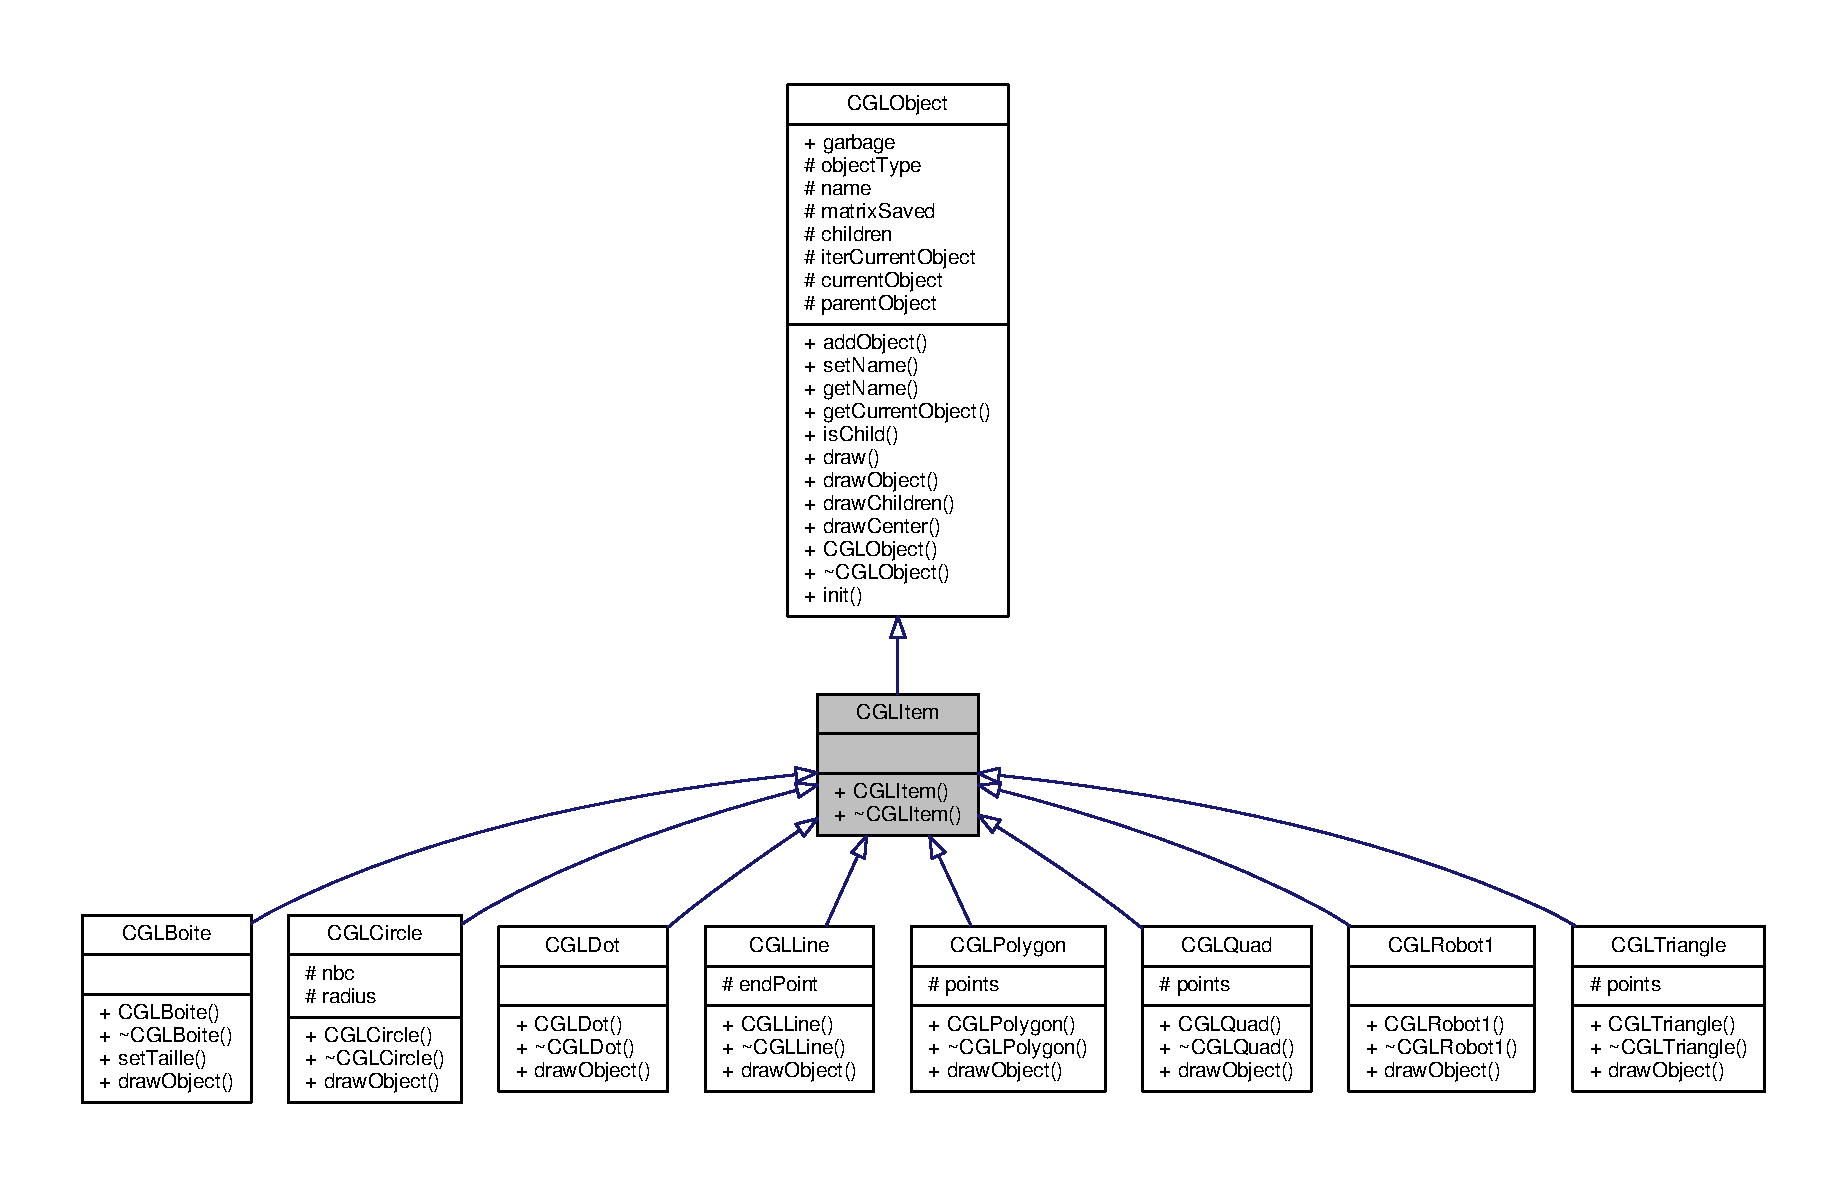
\includegraphics[width=350pt]{d3/d21/class_c_g_l_item__inherit__graph}
\end{center}
\end{figure}


Graphe de collaboration de C\-G\-L\-Item\-:\nopagebreak
\begin{figure}[H]
\begin{center}
\leavevmode
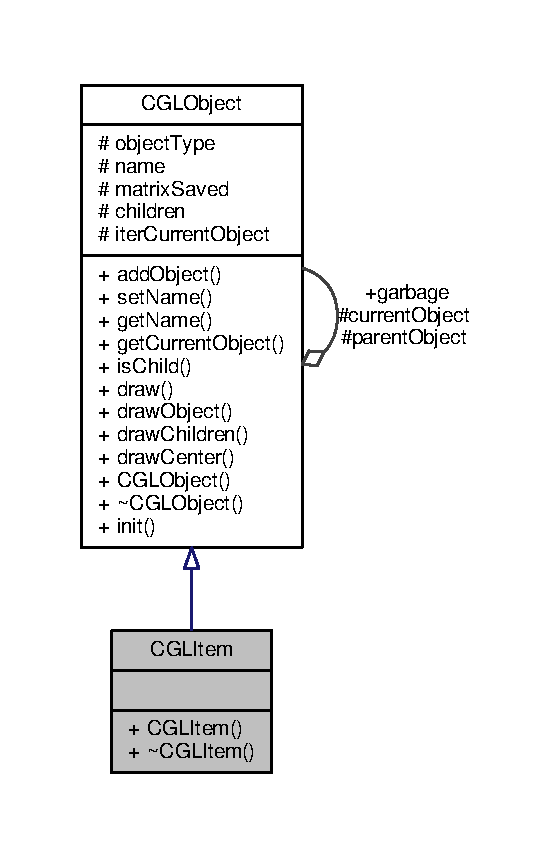
\includegraphics[width=267pt]{de/d34/class_c_g_l_item__coll__graph}
\end{center}
\end{figure}
\subsection*{Fonctions membres publiques}
\begin{DoxyCompactItemize}
\item 
\hyperlink{class_c_g_l_item_a263f620477dfb4e25e43ea6f011d6ff1}{C\-G\-L\-Item} ()
\item 
virtual \hyperlink{class_c_g_l_item_a4419eb1f52649a9267c5f236500377f2}{$\sim$\-C\-G\-L\-Item} ()
\end{DoxyCompactItemize}
\subsection*{Membres hérités additionnels}


\subsection{Description détaillée}


Définition à la ligne 17 du fichier C\-G\-L\-Item.\-h.



\subsection{Documentation des constructeurs et destructeur}
\hypertarget{class_c_g_l_item_a263f620477dfb4e25e43ea6f011d6ff1}{\index{C\-G\-L\-Item@{C\-G\-L\-Item}!C\-G\-L\-Item@{C\-G\-L\-Item}}
\index{C\-G\-L\-Item@{C\-G\-L\-Item}!CGLItem@{C\-G\-L\-Item}}
\subsubsection[{C\-G\-L\-Item}]{\setlength{\rightskip}{0pt plus 5cm}C\-G\-L\-Item\-::\-C\-G\-L\-Item (
\begin{DoxyParamCaption}
{}
\end{DoxyParamCaption}
)}}\label{class_c_g_l_item_a263f620477dfb4e25e43ea6f011d6ff1}


Définition à la ligne 10 du fichier C\-G\-L\-Item.\-cpp.

\hypertarget{class_c_g_l_item_a4419eb1f52649a9267c5f236500377f2}{\index{C\-G\-L\-Item@{C\-G\-L\-Item}!$\sim$\-C\-G\-L\-Item@{$\sim$\-C\-G\-L\-Item}}
\index{$\sim$\-C\-G\-L\-Item@{$\sim$\-C\-G\-L\-Item}!CGLItem@{C\-G\-L\-Item}}
\subsubsection[{$\sim$\-C\-G\-L\-Item}]{\setlength{\rightskip}{0pt plus 5cm}C\-G\-L\-Item\-::$\sim$\-C\-G\-L\-Item (
\begin{DoxyParamCaption}
{}
\end{DoxyParamCaption}
)\hspace{0.3cm}{\ttfamily [virtual]}}}\label{class_c_g_l_item_a4419eb1f52649a9267c5f236500377f2}


Définition à la ligne 15 du fichier C\-G\-L\-Item.\-cpp.



La documentation de cette classe a été générée à partir des fichiers suivants \-:\begin{DoxyCompactItemize}
\item 
/home/dagal/git/\-Damier\-G\-L/\-Damier\-G\-L/src/\-C\-G\-L/\hyperlink{_c_g_l_item_8h}{C\-G\-L\-Item.\-h}\item 
/home/dagal/git/\-Damier\-G\-L/\-Damier\-G\-L/src/\-C\-G\-L/\hyperlink{_c_g_l_item_8cpp}{C\-G\-L\-Item.\-cpp}\end{DoxyCompactItemize}

\hypertarget{class_c_g_l_light}{\section{Référence de la classe C\-G\-L\-Light}
\label{class_c_g_l_light}\index{C\-G\-L\-Light@{C\-G\-L\-Light}}
}


{\ttfamily \#include $<$C\-G\-L\-Light.\-h$>$}



Graphe de collaboration de C\-G\-L\-Light\-:\nopagebreak
\begin{figure}[H]
\begin{center}
\leavevmode
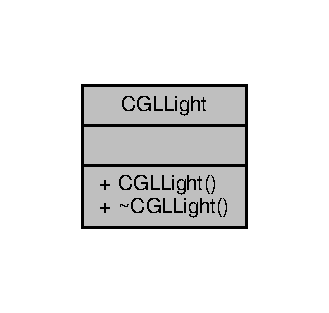
\includegraphics[width=158pt]{dd/d8c/class_c_g_l_light__coll__graph}
\end{center}
\end{figure}
\subsection*{Fonctions membres publiques}
\begin{DoxyCompactItemize}
\item 
\hyperlink{class_c_g_l_light_a1c792838909522f9f2b7c834d4ed2f25}{C\-G\-L\-Light} ()
\item 
virtual \hyperlink{class_c_g_l_light_add59dc580720d70fa5181c7de5ee5f7f}{$\sim$\-C\-G\-L\-Light} ()
\end{DoxyCompactItemize}


\subsection{Description détaillée}


Définition à la ligne 11 du fichier C\-G\-L\-Light.\-h.



\subsection{Documentation des constructeurs et destructeur}
\hypertarget{class_c_g_l_light_a1c792838909522f9f2b7c834d4ed2f25}{\index{C\-G\-L\-Light@{C\-G\-L\-Light}!C\-G\-L\-Light@{C\-G\-L\-Light}}
\index{C\-G\-L\-Light@{C\-G\-L\-Light}!CGLLight@{C\-G\-L\-Light}}
\subsubsection[{C\-G\-L\-Light}]{\setlength{\rightskip}{0pt plus 5cm}C\-G\-L\-Light\-::\-C\-G\-L\-Light (
\begin{DoxyParamCaption}
{}
\end{DoxyParamCaption}
)}}\label{class_c_g_l_light_a1c792838909522f9f2b7c834d4ed2f25}


Définition à la ligne 10 du fichier C\-G\-L\-Light.\-cpp.

\hypertarget{class_c_g_l_light_add59dc580720d70fa5181c7de5ee5f7f}{\index{C\-G\-L\-Light@{C\-G\-L\-Light}!$\sim$\-C\-G\-L\-Light@{$\sim$\-C\-G\-L\-Light}}
\index{$\sim$\-C\-G\-L\-Light@{$\sim$\-C\-G\-L\-Light}!CGLLight@{C\-G\-L\-Light}}
\subsubsection[{$\sim$\-C\-G\-L\-Light}]{\setlength{\rightskip}{0pt plus 5cm}C\-G\-L\-Light\-::$\sim$\-C\-G\-L\-Light (
\begin{DoxyParamCaption}
{}
\end{DoxyParamCaption}
)\hspace{0.3cm}{\ttfamily [virtual]}}}\label{class_c_g_l_light_add59dc580720d70fa5181c7de5ee5f7f}


Définition à la ligne 13 du fichier C\-G\-L\-Light.\-cpp.



La documentation de cette classe a été générée à partir des fichiers suivants \-:\begin{DoxyCompactItemize}
\item 
/home/dagal/git/\-Damier\-G\-L/\-Damier\-G\-L/src/\-C\-G\-L/\hyperlink{_c_g_l_light_8h}{C\-G\-L\-Light.\-h}\item 
/home/dagal/git/\-Damier\-G\-L/\-Damier\-G\-L/src/\-C\-G\-L/\hyperlink{_c_g_l_light_8cpp}{C\-G\-L\-Light.\-cpp}\end{DoxyCompactItemize}

\hypertarget{class_c_g_l_line}{\section{Référence de la classe C\-G\-L\-Line}
\label{class_c_g_l_line}\index{C\-G\-L\-Line@{C\-G\-L\-Line}}
}


{\ttfamily \#include $<$Line.\-h$>$}



Graphe d'héritage de C\-G\-L\-Line\-:
\nopagebreak
\begin{figure}[H]
\begin{center}
\leavevmode
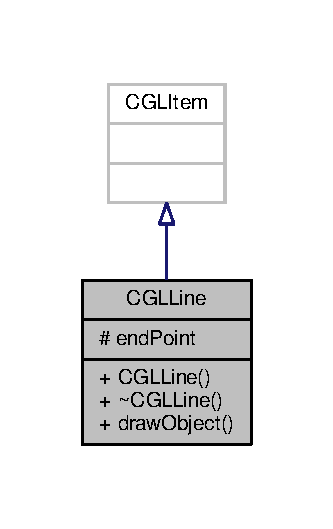
\includegraphics[width=160pt]{d9/dd7/class_c_g_l_line__inherit__graph}
\end{center}
\end{figure}


Graphe de collaboration de C\-G\-L\-Line\-:
\nopagebreak
\begin{figure}[H]
\begin{center}
\leavevmode
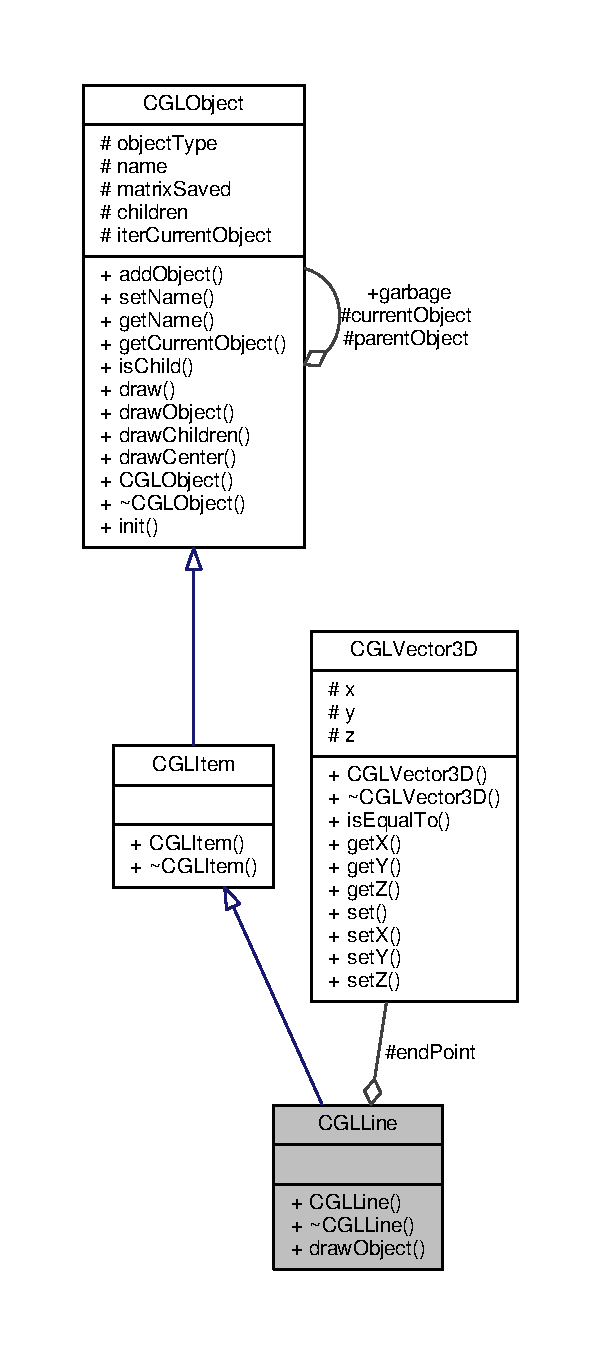
\includegraphics[width=160pt]{db/d95/class_c_g_l_line__coll__graph}
\end{center}
\end{figure}
\subsection*{Fonctions membres publiques}
\begin{DoxyCompactItemize}
\item 
\hyperlink{class_c_g_l_line_ab220112ce9d381cc057e6cff09fd95a7}{C\-G\-L\-Line} ()
\item 
virtual \hyperlink{class_c_g_l_line_ae00c52a8b8890cbe7657862aad150022}{$\sim$\-C\-G\-L\-Line} ()
\item 
void \hyperlink{class_c_g_l_line_a9621fa37a8b87f06e2a67aa8bf17d957}{draw\-Object} (Uint32 ellapsed\-Time)
\end{DoxyCompactItemize}
\subsection*{Attributs protégés}
\begin{DoxyCompactItemize}
\item 
C\-G\-L\-Vector3\-D \hyperlink{class_c_g_l_line_a2c4e6d2079bbac662dddf3fc137ad4d9}{end\-Point}
\end{DoxyCompactItemize}


\subsection{Description détaillée}


Définition à la ligne 17 du fichier Line.\-h.



\subsection{Documentation des constructeurs et destructeur}
\hypertarget{class_c_g_l_line_ab220112ce9d381cc057e6cff09fd95a7}{\index{C\-G\-L\-Line@{C\-G\-L\-Line}!C\-G\-L\-Line@{C\-G\-L\-Line}}
\index{C\-G\-L\-Line@{C\-G\-L\-Line}!CGLLine@{C\-G\-L\-Line}}
\subsubsection[{C\-G\-L\-Line}]{\setlength{\rightskip}{0pt plus 5cm}C\-G\-L\-Line\-::\-C\-G\-L\-Line (
\begin{DoxyParamCaption}
{}
\end{DoxyParamCaption}
)}}\label{class_c_g_l_line_ab220112ce9d381cc057e6cff09fd95a7}


Définition à la ligne 10 du fichier Line.\-cpp.

\hypertarget{class_c_g_l_line_ae00c52a8b8890cbe7657862aad150022}{\index{C\-G\-L\-Line@{C\-G\-L\-Line}!$\sim$\-C\-G\-L\-Line@{$\sim$\-C\-G\-L\-Line}}
\index{$\sim$\-C\-G\-L\-Line@{$\sim$\-C\-G\-L\-Line}!CGLLine@{C\-G\-L\-Line}}
\subsubsection[{$\sim$\-C\-G\-L\-Line}]{\setlength{\rightskip}{0pt plus 5cm}C\-G\-L\-Line\-::$\sim$\-C\-G\-L\-Line (
\begin{DoxyParamCaption}
{}
\end{DoxyParamCaption}
)\hspace{0.3cm}{\ttfamily [virtual]}}}\label{class_c_g_l_line_ae00c52a8b8890cbe7657862aad150022}


Définition à la ligne 15 du fichier Line.\-cpp.



\subsection{Documentation des fonctions membres}
\hypertarget{class_c_g_l_line_a9621fa37a8b87f06e2a67aa8bf17d957}{\index{C\-G\-L\-Line@{C\-G\-L\-Line}!draw\-Object@{draw\-Object}}
\index{draw\-Object@{draw\-Object}!CGLLine@{C\-G\-L\-Line}}
\subsubsection[{draw\-Object}]{\setlength{\rightskip}{0pt plus 5cm}void C\-G\-L\-Line\-::draw\-Object (
\begin{DoxyParamCaption}
\item[{Uint32}]{ellapsed\-Time}
\end{DoxyParamCaption}
)}}\label{class_c_g_l_line_a9621fa37a8b87f06e2a67aa8bf17d957}


Définition à la ligne 19 du fichier Line.\-cpp.



\subsection{Documentation des données membres}
\hypertarget{class_c_g_l_line_a2c4e6d2079bbac662dddf3fc137ad4d9}{\index{C\-G\-L\-Line@{C\-G\-L\-Line}!end\-Point@{end\-Point}}
\index{end\-Point@{end\-Point}!CGLLine@{C\-G\-L\-Line}}
\subsubsection[{end\-Point}]{\setlength{\rightskip}{0pt plus 5cm}C\-G\-L\-Vector3\-D C\-G\-L\-Line\-::end\-Point\hspace{0.3cm}{\ttfamily [protected]}}}\label{class_c_g_l_line_a2c4e6d2079bbac662dddf3fc137ad4d9}


Définition à la ligne 20 du fichier Line.\-h.



La documentation de cette classe a été générée à partir des fichiers suivants \-:\begin{DoxyCompactItemize}
\item 
/home/dagal/git/\-D\-G\-L/\-Damier\-G\-L/src/\-C\-G\-L/\hyperlink{_line_8h}{Line.\-h}\item 
/home/dagal/git/\-D\-G\-L/\-Damier\-G\-L/src/\-C\-G\-L/\hyperlink{_line_8cpp}{Line.\-cpp}\end{DoxyCompactItemize}

\hypertarget{class_c_g_l_object}{\section{Référence de la classe C\-G\-L\-Object}
\label{class_c_g_l_object}\index{C\-G\-L\-Object@{C\-G\-L\-Object}}
}


{\ttfamily \#include $<$C\-G\-L\-Object.\-h$>$}



Graphe d'héritage de C\-G\-L\-Object\-:
\nopagebreak
\begin{figure}[H]
\begin{center}
\leavevmode
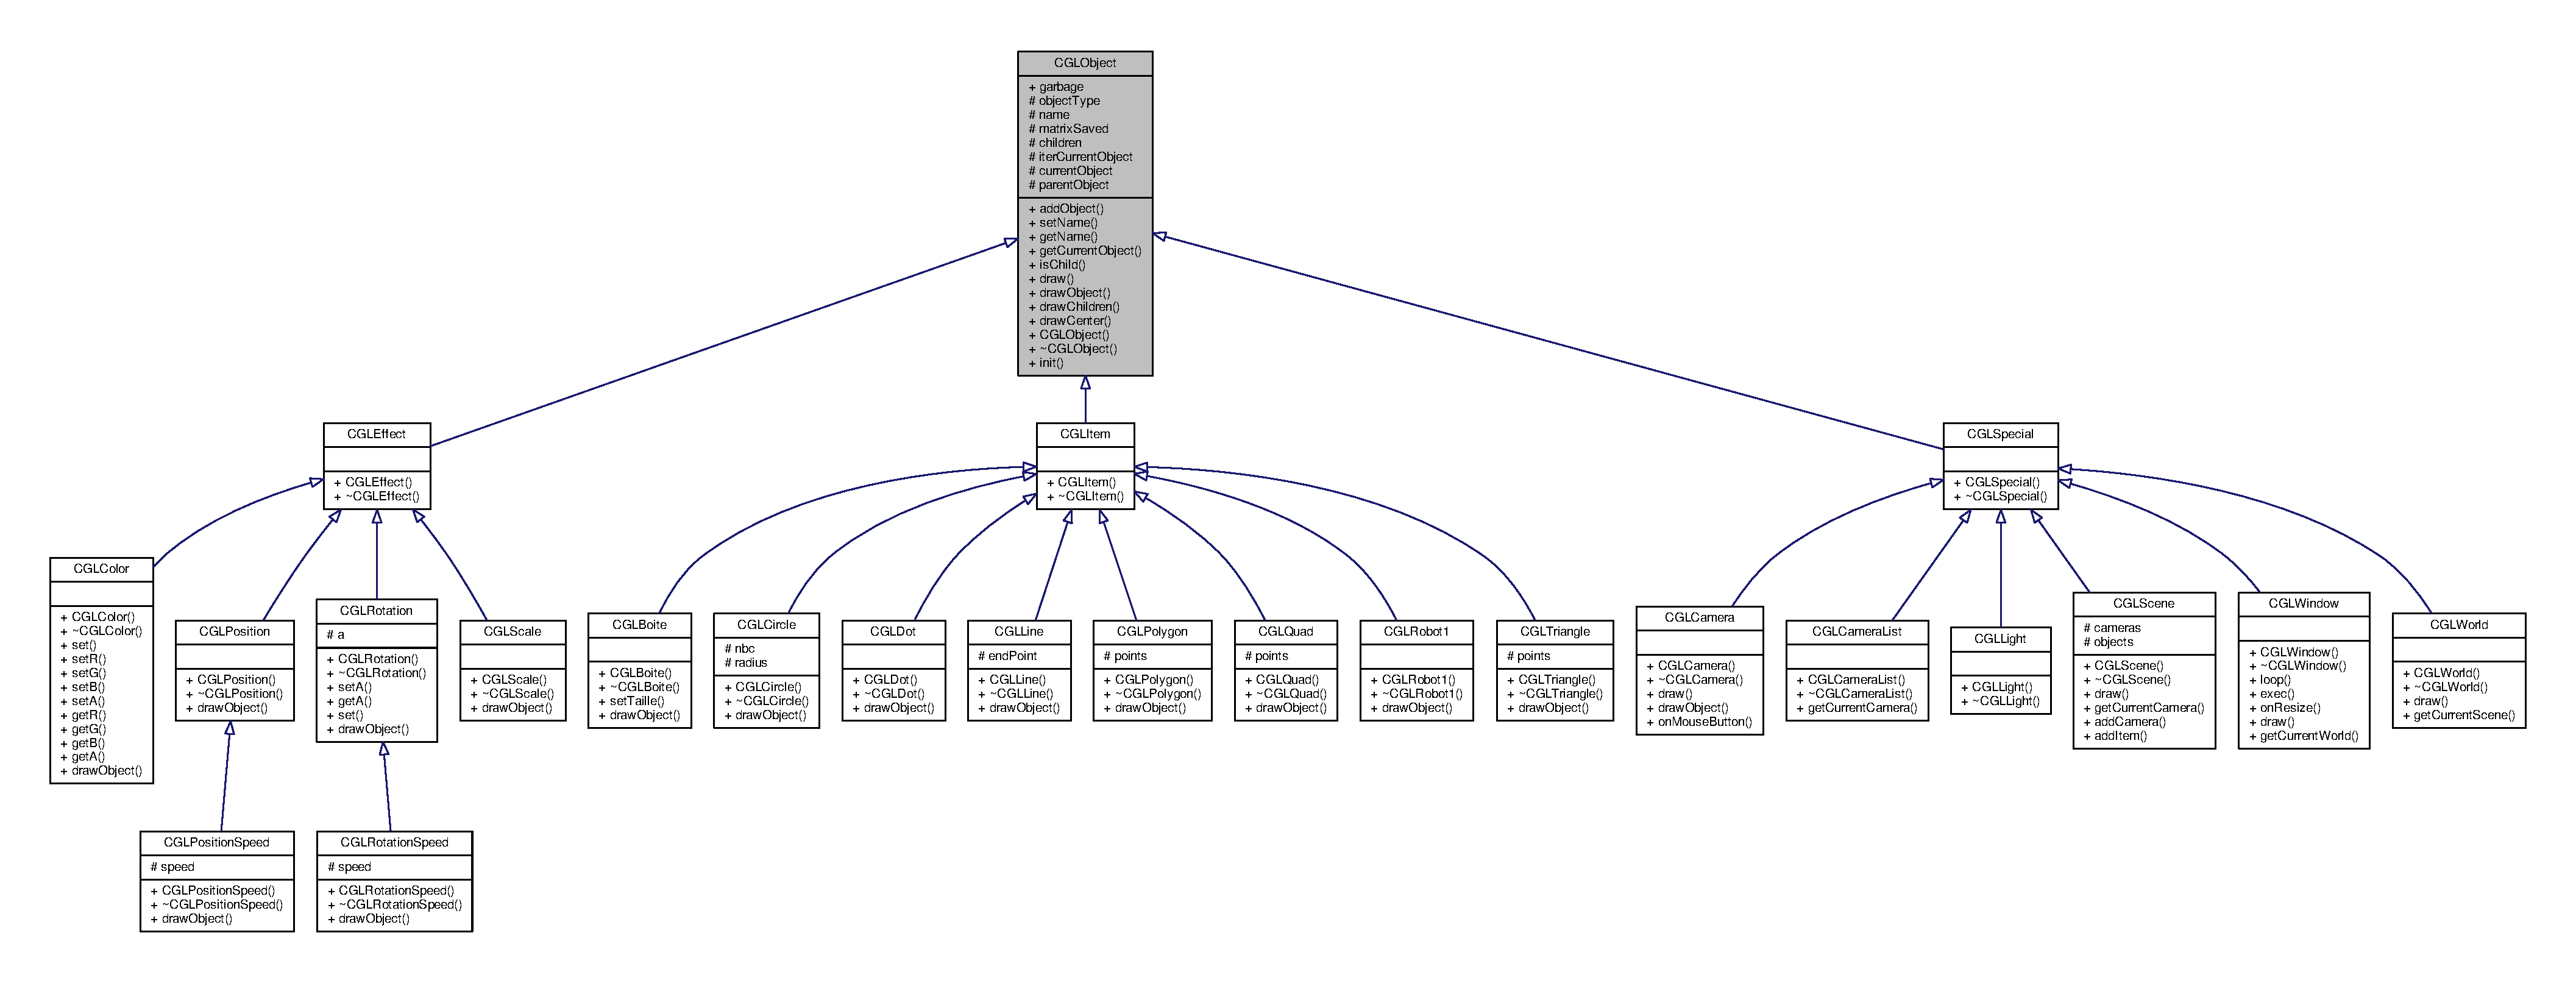
\includegraphics[width=350pt]{d8/d78/class_c_g_l_object__inherit__graph}
\end{center}
\end{figure}


Graphe de collaboration de C\-G\-L\-Object\-:\nopagebreak
\begin{figure}[H]
\begin{center}
\leavevmode
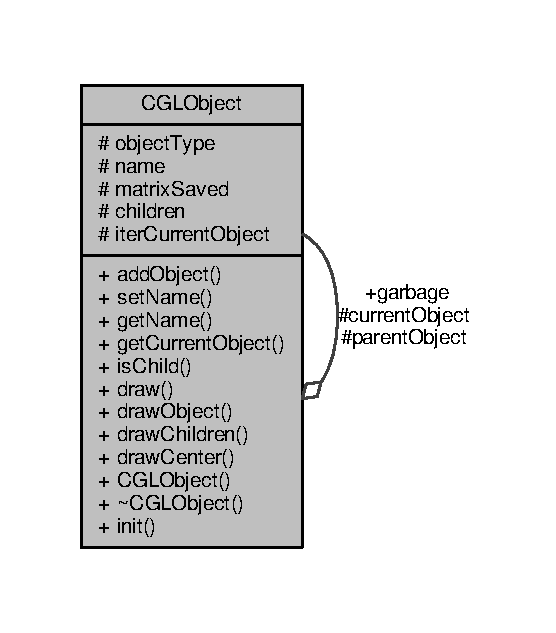
\includegraphics[width=267pt]{dd/dbf/class_c_g_l_object__coll__graph}
\end{center}
\end{figure}
\subsection*{Fonctions membres publiques}
\begin{DoxyCompactItemize}
\item 
void \hyperlink{class_c_g_l_object_a83b8918905a5449c94e4447791b61abd}{add\-Object} (\hyperlink{class_c_g_l_object}{C\-G\-L\-Object} $\ast$object)
\item 
void \hyperlink{class_c_g_l_object_aacbe6a176989b2cef7bc2be472d5c512}{set\-Name} (string n)
\item 
string \hyperlink{class_c_g_l_object_a98fea12fb2a998e0e13087c24fc9122a}{get\-Name} ()
\item 
\hyperlink{class_c_g_l_object}{C\-G\-L\-Object} $\ast$ \hyperlink{class_c_g_l_object_a17159bf8a16301adca577be4311806d1}{get\-Current\-Object} ()
\item 
bool \hyperlink{class_c_g_l_object_a80d01439776edc9443b47a7a9e5b9e94}{is\-Child} (\hyperlink{class_c_g_l_object}{C\-G\-L\-Object} $\ast$obj)
\item 
void \hyperlink{class_c_g_l_object_a39c4cde56d18140384842d074407c5c4}{draw} (Uint32 time\-Ellapsed)
\item 
virtual void \hyperlink{class_c_g_l_object_a2781ec98c37bd209f2382c5130a365b9}{draw\-Object} (Uint32 time\-Ellapsed)
\item 
void \hyperlink{class_c_g_l_object_a6c23675f91b2adc88a95d6da869652d4}{draw\-Children} (Uint32 time\-Ellapsed)
\item 
void \hyperlink{class_c_g_l_object_a310a26c3464c16c7b08349fe41123364}{draw\-Center} ()
\item 
\hyperlink{class_c_g_l_object_add00987cd4a5ee06cc4436766392434b}{C\-G\-L\-Object} ()
\item 
virtual \hyperlink{class_c_g_l_object_aa92f9815a1cc5d563b991a5ed786bd5e}{$\sim$\-C\-G\-L\-Object} ()
\end{DoxyCompactItemize}
\subsection*{Fonctions membres publiques statiques}
\begin{DoxyCompactItemize}
\item 
static void \hyperlink{class_c_g_l_object_aa08cbbe873bf264dbb34f233bd21844b}{init} ()
\end{DoxyCompactItemize}
\subsection*{Attributs publics statiques}
\begin{DoxyCompactItemize}
\item 
static \hyperlink{class_c_g_l_object}{C\-G\-L\-Object} $\ast$ \hyperlink{class_c_g_l_object_aa042ffd6be6c676dd6fa779c2e23752d}{garbage} = N\-U\-L\-L
\end{DoxyCompactItemize}
\subsection*{Attributs protégés}
\begin{DoxyCompactItemize}
\item 
int \hyperlink{class_c_g_l_object_a5ff11ea98cb278213849d6a6f4124cdc}{object\-Type}
\item 
string \hyperlink{class_c_g_l_object_a0397e47d30fd9a5eb57cce07e4b02bce}{name}
\item 
bool \hyperlink{class_c_g_l_object_a82401873b76121a112af9b824a661ba1}{matrix\-Saved}
\item 
list$<$ \hyperlink{class_c_g_l_object}{C\-G\-L\-Object} $\ast$ $>$ \hyperlink{class_c_g_l_object_ac7dc91801d4a50f24e1624283a7a3190}{children}
\item 
list$<$ \hyperlink{class_c_g_l_object}{C\-G\-L\-Object} $\ast$ $>$\-::iterator \hyperlink{class_c_g_l_object_a9e1debfc7948f902f40d07a7da209203}{iter\-Current\-Object}
\item 
\hyperlink{class_c_g_l_object}{C\-G\-L\-Object} $\ast$ \hyperlink{class_c_g_l_object_a3e0d024fd6deb36518196f57aab75d2b}{current\-Object}
\item 
\hyperlink{class_c_g_l_object}{C\-G\-L\-Object} $\ast$ \hyperlink{class_c_g_l_object_a445899f0f0a263df4780ccf75103c2a9}{parent\-Object}
\end{DoxyCompactItemize}


\subsection{Description détaillée}
Classe de base de la bibliothèque 

Définition à la ligne 25 du fichier C\-G\-L\-Object.\-h.



\subsection{Documentation des constructeurs et destructeur}
\hypertarget{class_c_g_l_object_add00987cd4a5ee06cc4436766392434b}{\index{C\-G\-L\-Object@{C\-G\-L\-Object}!C\-G\-L\-Object@{C\-G\-L\-Object}}
\index{C\-G\-L\-Object@{C\-G\-L\-Object}!CGLObject@{C\-G\-L\-Object}}
\subsubsection[{C\-G\-L\-Object}]{\setlength{\rightskip}{0pt plus 5cm}C\-G\-L\-Object\-::\-C\-G\-L\-Object (
\begin{DoxyParamCaption}
{}
\end{DoxyParamCaption}
)}}\label{class_c_g_l_object_add00987cd4a5ee06cc4436766392434b}
Prépare tout pour vous… 

Définition à la ligne 15 du fichier C\-G\-L\-Object.\-cpp.



Voici le graphe d'appel pour cette fonction \-:\nopagebreak
\begin{figure}[H]
\begin{center}
\leavevmode
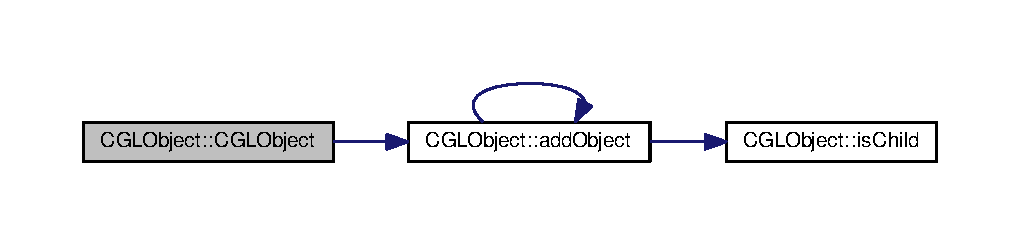
\includegraphics[width=350pt]{d2/d76/class_c_g_l_object_add00987cd4a5ee06cc4436766392434b_cgraph}
\end{center}
\end{figure}




Voici le graphe des appelants de cette fonction \-:\nopagebreak
\begin{figure}[H]
\begin{center}
\leavevmode
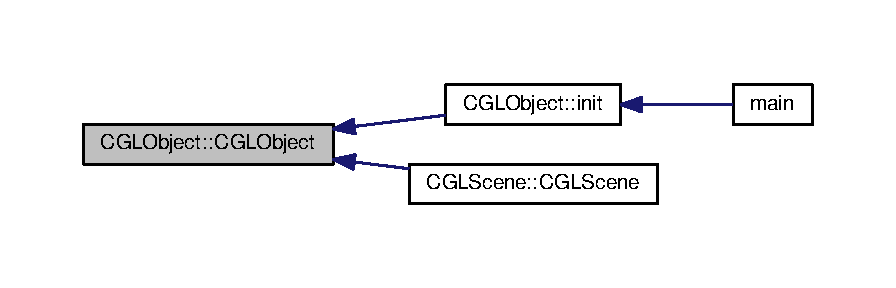
\includegraphics[width=350pt]{d2/d76/class_c_g_l_object_add00987cd4a5ee06cc4436766392434b_icgraph}
\end{center}
\end{figure}


\hypertarget{class_c_g_l_object_aa92f9815a1cc5d563b991a5ed786bd5e}{\index{C\-G\-L\-Object@{C\-G\-L\-Object}!$\sim$\-C\-G\-L\-Object@{$\sim$\-C\-G\-L\-Object}}
\index{$\sim$\-C\-G\-L\-Object@{$\sim$\-C\-G\-L\-Object}!CGLObject@{C\-G\-L\-Object}}
\subsubsection[{$\sim$\-C\-G\-L\-Object}]{\setlength{\rightskip}{0pt plus 5cm}C\-G\-L\-Object\-::$\sim$\-C\-G\-L\-Object (
\begin{DoxyParamCaption}
{}
\end{DoxyParamCaption}
)\hspace{0.3cm}{\ttfamily [virtual]}}}\label{class_c_g_l_object_aa92f9815a1cc5d563b991a5ed786bd5e}


Définition à la ligne 29 du fichier C\-G\-L\-Object.\-cpp.



\subsection{Documentation des fonctions membres}
\hypertarget{class_c_g_l_object_a83b8918905a5449c94e4447791b61abd}{\index{C\-G\-L\-Object@{C\-G\-L\-Object}!add\-Object@{add\-Object}}
\index{add\-Object@{add\-Object}!CGLObject@{C\-G\-L\-Object}}
\subsubsection[{add\-Object}]{\setlength{\rightskip}{0pt plus 5cm}void C\-G\-L\-Object\-::add\-Object (
\begin{DoxyParamCaption}
\item[{{\bf C\-G\-L\-Object} $\ast$}]{object}
\end{DoxyParamCaption}
)}}\label{class_c_g_l_object_a83b8918905a5449c94e4447791b61abd}


Définition à la ligne 58 du fichier C\-G\-L\-Object.\-cpp.



Voici le graphe d'appel pour cette fonction \-:\nopagebreak
\begin{figure}[H]
\begin{center}
\leavevmode
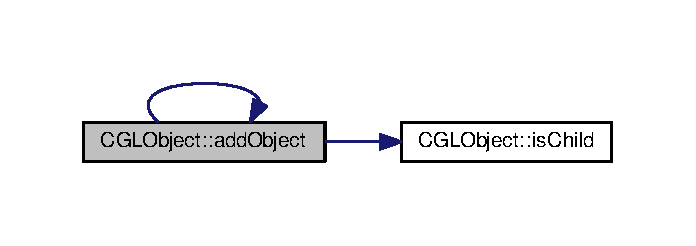
\includegraphics[width=334pt]{d2/d76/class_c_g_l_object_a83b8918905a5449c94e4447791b61abd_cgraph}
\end{center}
\end{figure}




Voici le graphe des appelants de cette fonction \-:\nopagebreak
\begin{figure}[H]
\begin{center}
\leavevmode
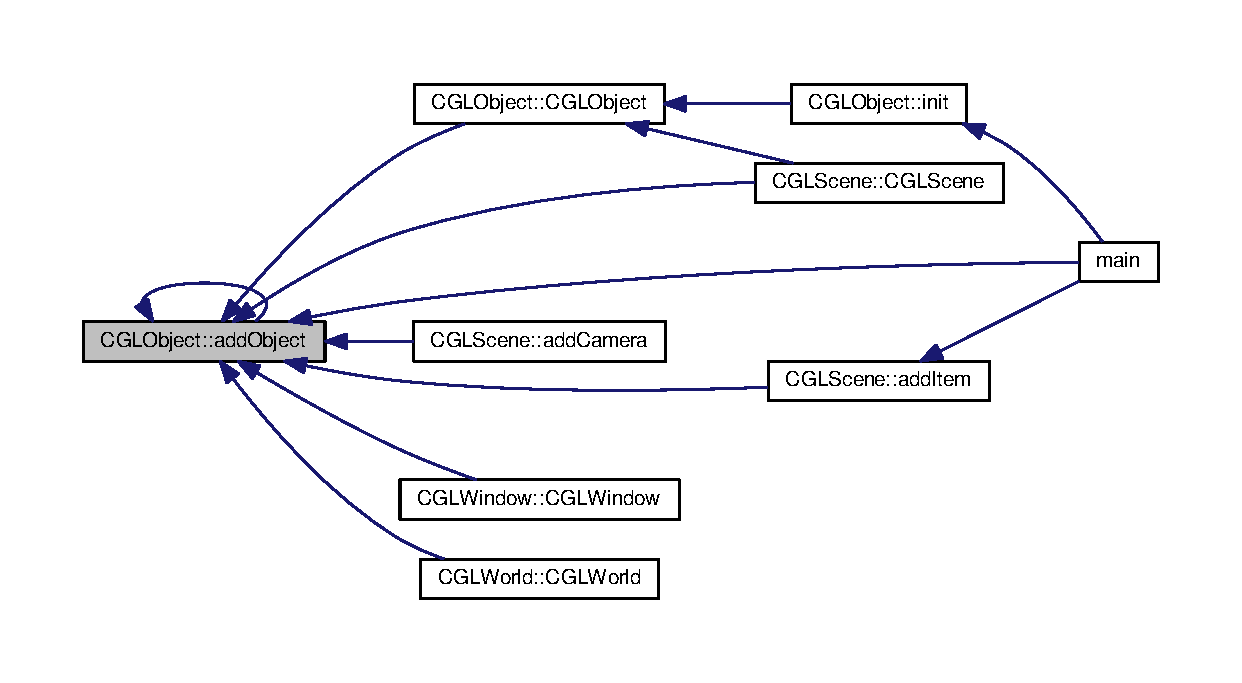
\includegraphics[width=350pt]{d2/d76/class_c_g_l_object_a83b8918905a5449c94e4447791b61abd_icgraph}
\end{center}
\end{figure}


\hypertarget{class_c_g_l_object_a39c4cde56d18140384842d074407c5c4}{\index{C\-G\-L\-Object@{C\-G\-L\-Object}!draw@{draw}}
\index{draw@{draw}!CGLObject@{C\-G\-L\-Object}}
\subsubsection[{draw}]{\setlength{\rightskip}{0pt plus 5cm}void C\-G\-L\-Object\-::draw (
\begin{DoxyParamCaption}
\item[{Uint32}]{time\-Ellapsed}
\end{DoxyParamCaption}
)}}\label{class_c_g_l_object_a39c4cde56d18140384842d074407c5c4}


Définition à la ligne 33 du fichier C\-G\-L\-Object.\-cpp.



Voici le graphe d'appel pour cette fonction \-:\nopagebreak
\begin{figure}[H]
\begin{center}
\leavevmode
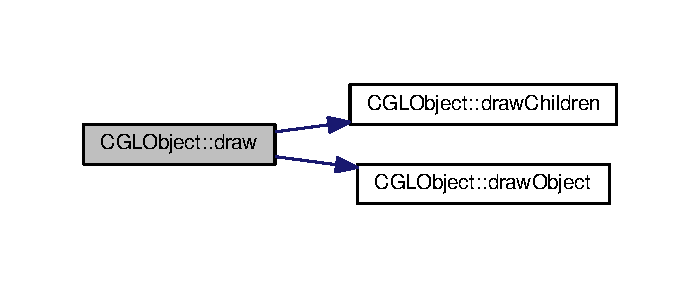
\includegraphics[width=336pt]{d2/d76/class_c_g_l_object_a39c4cde56d18140384842d074407c5c4_cgraph}
\end{center}
\end{figure}




Voici le graphe des appelants de cette fonction \-:\nopagebreak
\begin{figure}[H]
\begin{center}
\leavevmode
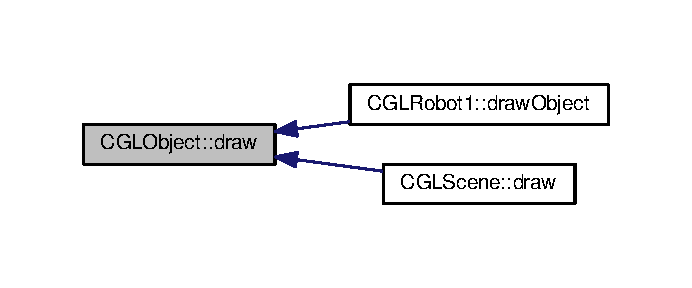
\includegraphics[width=332pt]{d2/d76/class_c_g_l_object_a39c4cde56d18140384842d074407c5c4_icgraph}
\end{center}
\end{figure}


\hypertarget{class_c_g_l_object_a310a26c3464c16c7b08349fe41123364}{\index{C\-G\-L\-Object@{C\-G\-L\-Object}!draw\-Center@{draw\-Center}}
\index{draw\-Center@{draw\-Center}!CGLObject@{C\-G\-L\-Object}}
\subsubsection[{draw\-Center}]{\setlength{\rightskip}{0pt plus 5cm}void C\-G\-L\-Object\-::draw\-Center (
\begin{DoxyParamCaption}
{}
\end{DoxyParamCaption}
)}}\label{class_c_g_l_object_a310a26c3464c16c7b08349fe41123364}


Définition à la ligne 47 du fichier C\-G\-L\-Object.\-cpp.

\hypertarget{class_c_g_l_object_a6c23675f91b2adc88a95d6da869652d4}{\index{C\-G\-L\-Object@{C\-G\-L\-Object}!draw\-Children@{draw\-Children}}
\index{draw\-Children@{draw\-Children}!CGLObject@{C\-G\-L\-Object}}
\subsubsection[{draw\-Children}]{\setlength{\rightskip}{0pt plus 5cm}void C\-G\-L\-Object\-::draw\-Children (
\begin{DoxyParamCaption}
\item[{Uint32}]{time\-Ellapsed}
\end{DoxyParamCaption}
)}}\label{class_c_g_l_object_a6c23675f91b2adc88a95d6da869652d4}


Définition à la ligne 75 du fichier C\-G\-L\-Object.\-cpp.



Voici le graphe des appelants de cette fonction \-:\nopagebreak
\begin{figure}[H]
\begin{center}
\leavevmode
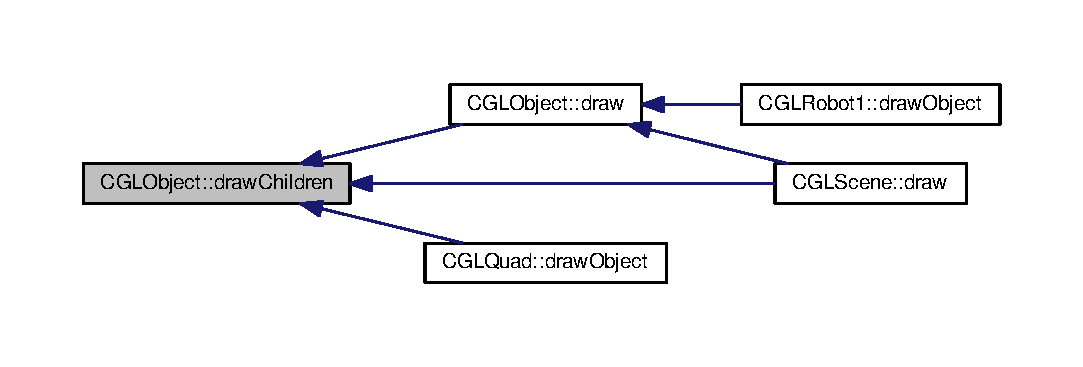
\includegraphics[width=350pt]{d2/d76/class_c_g_l_object_a6c23675f91b2adc88a95d6da869652d4_icgraph}
\end{center}
\end{figure}


\hypertarget{class_c_g_l_object_a2781ec98c37bd209f2382c5130a365b9}{\index{C\-G\-L\-Object@{C\-G\-L\-Object}!draw\-Object@{draw\-Object}}
\index{draw\-Object@{draw\-Object}!CGLObject@{C\-G\-L\-Object}}
\subsubsection[{draw\-Object}]{\setlength{\rightskip}{0pt plus 5cm}void C\-G\-L\-Object\-::draw\-Object (
\begin{DoxyParamCaption}
\item[{Uint32}]{time\-Ellapsed}
\end{DoxyParamCaption}
)\hspace{0.3cm}{\ttfamily [virtual]}}}\label{class_c_g_l_object_a2781ec98c37bd209f2382c5130a365b9}


Réimplémentée dans \hyperlink{class_c_g_l_color_a69d92c401c12b7846c458c41a564b3ae}{C\-G\-L\-Color}, \hyperlink{class_c_g_l_camera_a804d27abd87be682a5b508fe5f0a4451}{C\-G\-L\-Camera}, \hyperlink{class_c_g_l_position_a439ae873ba7ef56826a27eb7b15b0b6f}{C\-G\-L\-Position}, \hyperlink{class_c_g_l_rotation_a94be2c089fbe52d0f8cb33ee98f8de74}{C\-G\-L\-Rotation}, \hyperlink{class_c_g_l_polygon_a8450b134d7e40059c36ecc43133596c0}{C\-G\-L\-Polygon}, \hyperlink{class_c_g_l_robot1_a050d7fea4097a6634ef5feef26ae7865}{C\-G\-L\-Robot1}, \hyperlink{class_c_g_l_circle_a222f67da86a92a075011ec607154b1f8}{C\-G\-L\-Circle}, \hyperlink{class_c_g_l_quad_a81696d558e2355af7d621cdbf0ccf41a}{C\-G\-L\-Quad}, \hyperlink{class_c_g_l_triangle_aab44f7f6fca4ad4cca693205aeb92fe3}{C\-G\-L\-Triangle}, \hyperlink{class_c_g_l_line_a9621fa37a8b87f06e2a67aa8bf17d957}{C\-G\-L\-Line}, \hyperlink{class_c_g_l_rotation_speed_a6549d856fc0ad620fd1507744104797f}{C\-G\-L\-Rotation\-Speed}, \hyperlink{class_c_g_l_scale_a27939db2fb5f900800f391bb06a387a4}{C\-G\-L\-Scale}, \hyperlink{class_c_g_l_boite_adc20f63de77be2f8a93500f0065b5e27}{C\-G\-L\-Boite}, et \hyperlink{class_c_g_l_dot_aba6d02d4c9da30aea263599e66e5f201}{C\-G\-L\-Dot}.



Définition à la ligne 43 du fichier C\-G\-L\-Object.\-cpp.



Voici le graphe des appelants de cette fonction \-:\nopagebreak
\begin{figure}[H]
\begin{center}
\leavevmode
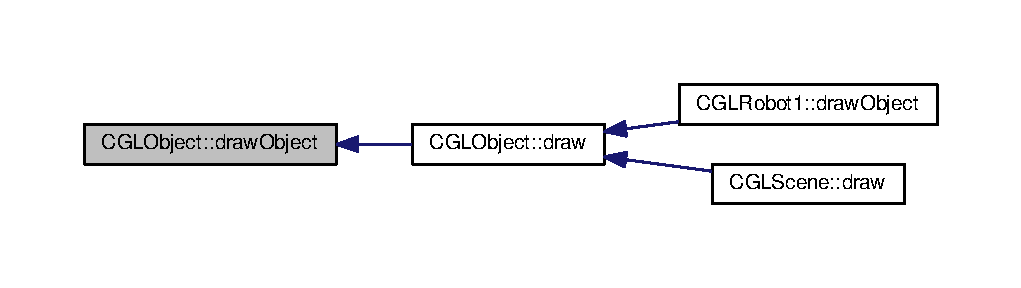
\includegraphics[width=350pt]{d2/d76/class_c_g_l_object_a2781ec98c37bd209f2382c5130a365b9_icgraph}
\end{center}
\end{figure}


\hypertarget{class_c_g_l_object_a17159bf8a16301adca577be4311806d1}{\index{C\-G\-L\-Object@{C\-G\-L\-Object}!get\-Current\-Object@{get\-Current\-Object}}
\index{get\-Current\-Object@{get\-Current\-Object}!CGLObject@{C\-G\-L\-Object}}
\subsubsection[{get\-Current\-Object}]{\setlength{\rightskip}{0pt plus 5cm}{\bf C\-G\-L\-Object} $\ast$ C\-G\-L\-Object\-::get\-Current\-Object (
\begin{DoxyParamCaption}
{}
\end{DoxyParamCaption}
)}}\label{class_c_g_l_object_a17159bf8a16301adca577be4311806d1}


Définition à la ligne 94 du fichier C\-G\-L\-Object.\-cpp.



Voici le graphe des appelants de cette fonction \-:\nopagebreak
\begin{figure}[H]
\begin{center}
\leavevmode
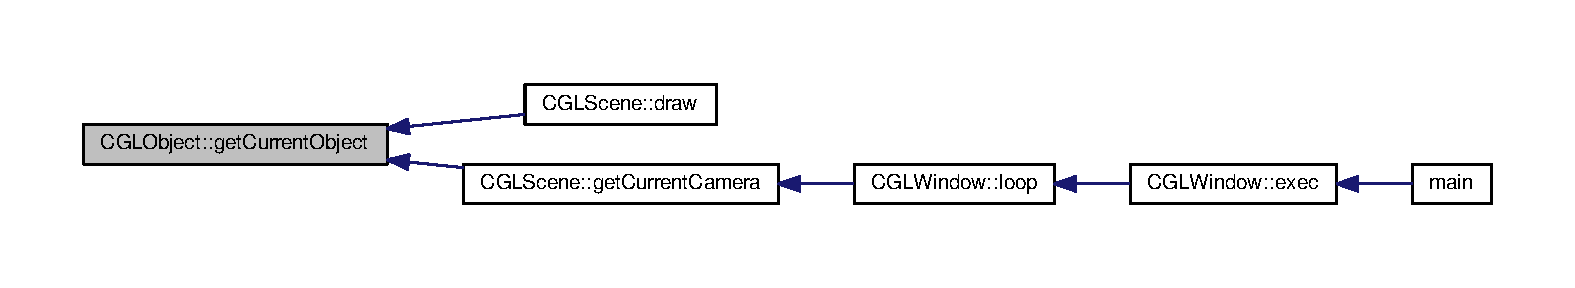
\includegraphics[width=350pt]{d2/d76/class_c_g_l_object_a17159bf8a16301adca577be4311806d1_icgraph}
\end{center}
\end{figure}


\hypertarget{class_c_g_l_object_a98fea12fb2a998e0e13087c24fc9122a}{\index{C\-G\-L\-Object@{C\-G\-L\-Object}!get\-Name@{get\-Name}}
\index{get\-Name@{get\-Name}!CGLObject@{C\-G\-L\-Object}}
\subsubsection[{get\-Name}]{\setlength{\rightskip}{0pt plus 5cm}string C\-G\-L\-Object\-::get\-Name (
\begin{DoxyParamCaption}
{}
\end{DoxyParamCaption}
)}}\label{class_c_g_l_object_a98fea12fb2a998e0e13087c24fc9122a}


Définition à la ligne 89 du fichier C\-G\-L\-Object.\-cpp.

\hypertarget{class_c_g_l_object_aa08cbbe873bf264dbb34f233bd21844b}{\index{C\-G\-L\-Object@{C\-G\-L\-Object}!init@{init}}
\index{init@{init}!CGLObject@{C\-G\-L\-Object}}
\subsubsection[{init}]{\setlength{\rightskip}{0pt plus 5cm}void C\-G\-L\-Object\-::init (
\begin{DoxyParamCaption}
{}
\end{DoxyParamCaption}
)\hspace{0.3cm}{\ttfamily [static]}}}\label{class_c_g_l_object_aa08cbbe873bf264dbb34f233bd21844b}


Définition à la ligne 99 du fichier C\-G\-L\-Object.\-cpp.



Voici le graphe d'appel pour cette fonction \-:\nopagebreak
\begin{figure}[H]
\begin{center}
\leavevmode
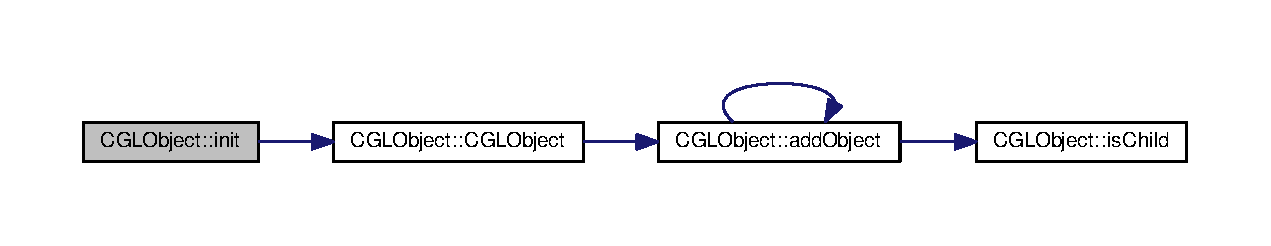
\includegraphics[width=350pt]{d2/d76/class_c_g_l_object_aa08cbbe873bf264dbb34f233bd21844b_cgraph}
\end{center}
\end{figure}




Voici le graphe des appelants de cette fonction \-:\nopagebreak
\begin{figure}[H]
\begin{center}
\leavevmode
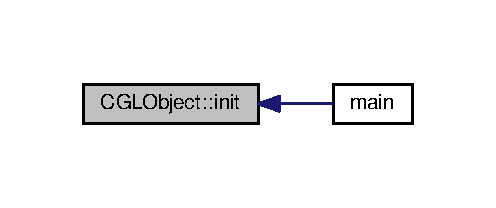
\includegraphics[width=238pt]{d2/d76/class_c_g_l_object_aa08cbbe873bf264dbb34f233bd21844b_icgraph}
\end{center}
\end{figure}


\hypertarget{class_c_g_l_object_a80d01439776edc9443b47a7a9e5b9e94}{\index{C\-G\-L\-Object@{C\-G\-L\-Object}!is\-Child@{is\-Child}}
\index{is\-Child@{is\-Child}!CGLObject@{C\-G\-L\-Object}}
\subsubsection[{is\-Child}]{\setlength{\rightskip}{0pt plus 5cm}bool C\-G\-L\-Object\-::is\-Child (
\begin{DoxyParamCaption}
\item[{{\bf C\-G\-L\-Object} $\ast$}]{obj}
\end{DoxyParamCaption}
)}}\label{class_c_g_l_object_a80d01439776edc9443b47a7a9e5b9e94}


Définition à la ligne 107 du fichier C\-G\-L\-Object.\-cpp.



Voici le graphe des appelants de cette fonction \-:\nopagebreak
\begin{figure}[H]
\begin{center}
\leavevmode
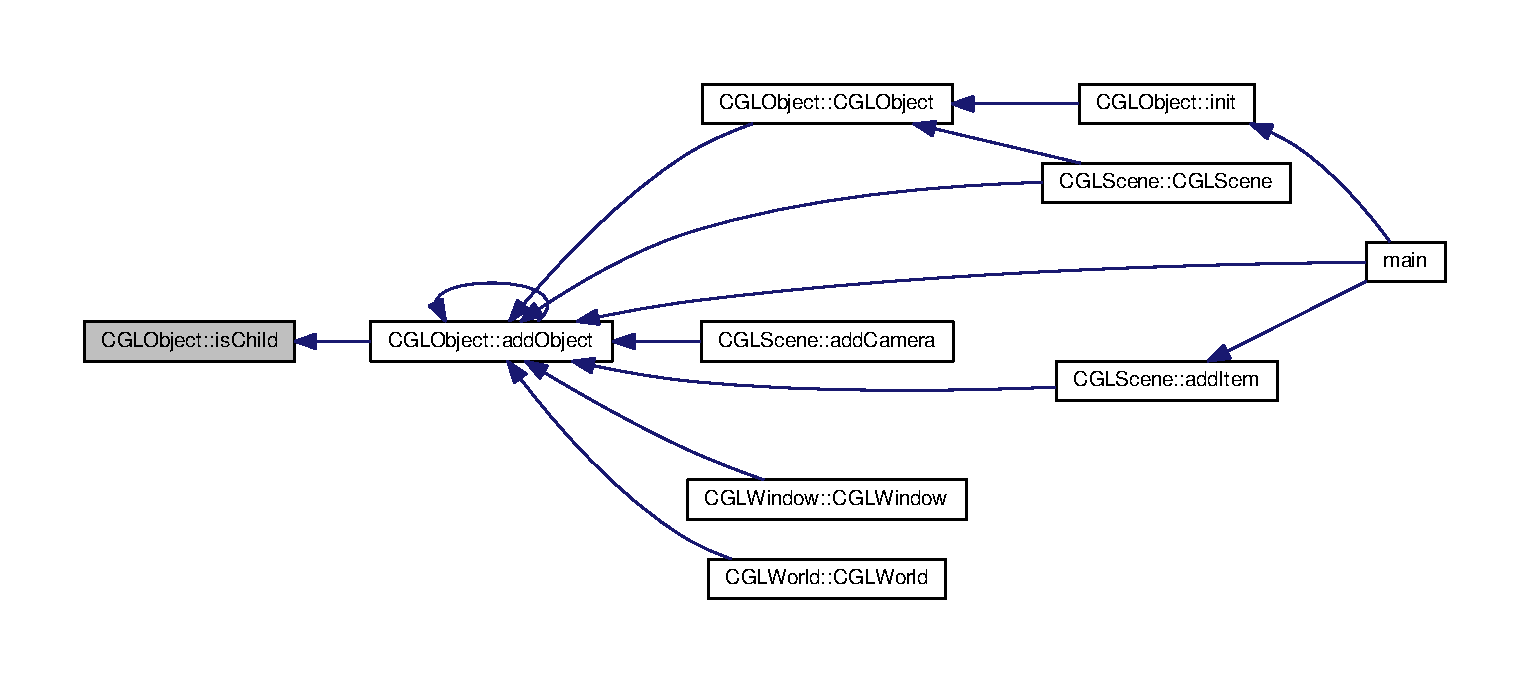
\includegraphics[width=350pt]{d2/d76/class_c_g_l_object_a80d01439776edc9443b47a7a9e5b9e94_icgraph}
\end{center}
\end{figure}


\hypertarget{class_c_g_l_object_aacbe6a176989b2cef7bc2be472d5c512}{\index{C\-G\-L\-Object@{C\-G\-L\-Object}!set\-Name@{set\-Name}}
\index{set\-Name@{set\-Name}!CGLObject@{C\-G\-L\-Object}}
\subsubsection[{set\-Name}]{\setlength{\rightskip}{0pt plus 5cm}void C\-G\-L\-Object\-::set\-Name (
\begin{DoxyParamCaption}
\item[{string}]{n}
\end{DoxyParamCaption}
)}}\label{class_c_g_l_object_aacbe6a176989b2cef7bc2be472d5c512}


Définition à la ligne 84 du fichier C\-G\-L\-Object.\-cpp.



Voici le graphe des appelants de cette fonction \-:\nopagebreak
\begin{figure}[H]
\begin{center}
\leavevmode
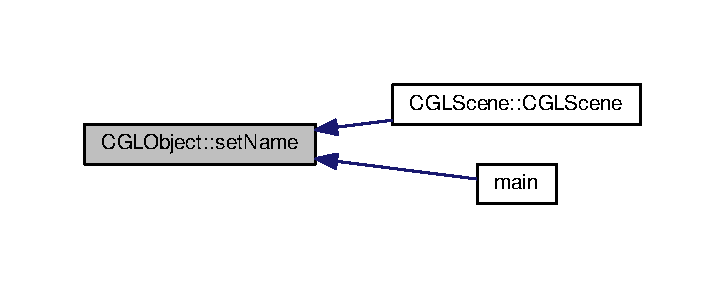
\includegraphics[width=348pt]{d2/d76/class_c_g_l_object_aacbe6a176989b2cef7bc2be472d5c512_icgraph}
\end{center}
\end{figure}




\subsection{Documentation des données membres}
\hypertarget{class_c_g_l_object_ac7dc91801d4a50f24e1624283a7a3190}{\index{C\-G\-L\-Object@{C\-G\-L\-Object}!children@{children}}
\index{children@{children}!CGLObject@{C\-G\-L\-Object}}
\subsubsection[{children}]{\setlength{\rightskip}{0pt plus 5cm}list$<${\bf C\-G\-L\-Object} $\ast$$>$ C\-G\-L\-Object\-::children\hspace{0.3cm}{\ttfamily [protected]}}}\label{class_c_g_l_object_ac7dc91801d4a50f24e1624283a7a3190}


Définition à la ligne 36 du fichier C\-G\-L\-Object.\-h.

\hypertarget{class_c_g_l_object_a3e0d024fd6deb36518196f57aab75d2b}{\index{C\-G\-L\-Object@{C\-G\-L\-Object}!current\-Object@{current\-Object}}
\index{current\-Object@{current\-Object}!CGLObject@{C\-G\-L\-Object}}
\subsubsection[{current\-Object}]{\setlength{\rightskip}{0pt plus 5cm}{\bf C\-G\-L\-Object}$\ast$ C\-G\-L\-Object\-::current\-Object\hspace{0.3cm}{\ttfamily [protected]}}}\label{class_c_g_l_object_a3e0d024fd6deb36518196f57aab75d2b}


Définition à la ligne 38 du fichier C\-G\-L\-Object.\-h.

\hypertarget{class_c_g_l_object_aa042ffd6be6c676dd6fa779c2e23752d}{\index{C\-G\-L\-Object@{C\-G\-L\-Object}!garbage@{garbage}}
\index{garbage@{garbage}!CGLObject@{C\-G\-L\-Object}}
\subsubsection[{garbage}]{\setlength{\rightskip}{0pt plus 5cm}{\bf C\-G\-L\-Object} $\ast$ C\-G\-L\-Object\-::garbage = N\-U\-L\-L\hspace{0.3cm}{\ttfamily [static]}}}\label{class_c_g_l_object_aa042ffd6be6c676dd6fa779c2e23752d}


Définition à la ligne 43 du fichier C\-G\-L\-Object.\-h.

\hypertarget{class_c_g_l_object_a9e1debfc7948f902f40d07a7da209203}{\index{C\-G\-L\-Object@{C\-G\-L\-Object}!iter\-Current\-Object@{iter\-Current\-Object}}
\index{iter\-Current\-Object@{iter\-Current\-Object}!CGLObject@{C\-G\-L\-Object}}
\subsubsection[{iter\-Current\-Object}]{\setlength{\rightskip}{0pt plus 5cm}list$<${\bf C\-G\-L\-Object} $\ast$$>$\-::iterator C\-G\-L\-Object\-::iter\-Current\-Object\hspace{0.3cm}{\ttfamily [protected]}}}\label{class_c_g_l_object_a9e1debfc7948f902f40d07a7da209203}


Définition à la ligne 37 du fichier C\-G\-L\-Object.\-h.

\hypertarget{class_c_g_l_object_a82401873b76121a112af9b824a661ba1}{\index{C\-G\-L\-Object@{C\-G\-L\-Object}!matrix\-Saved@{matrix\-Saved}}
\index{matrix\-Saved@{matrix\-Saved}!CGLObject@{C\-G\-L\-Object}}
\subsubsection[{matrix\-Saved}]{\setlength{\rightskip}{0pt plus 5cm}bool C\-G\-L\-Object\-::matrix\-Saved\hspace{0.3cm}{\ttfamily [protected]}}}\label{class_c_g_l_object_a82401873b76121a112af9b824a661ba1}


Définition à la ligne 34 du fichier C\-G\-L\-Object.\-h.

\hypertarget{class_c_g_l_object_a0397e47d30fd9a5eb57cce07e4b02bce}{\index{C\-G\-L\-Object@{C\-G\-L\-Object}!name@{name}}
\index{name@{name}!CGLObject@{C\-G\-L\-Object}}
\subsubsection[{name}]{\setlength{\rightskip}{0pt plus 5cm}string C\-G\-L\-Object\-::name\hspace{0.3cm}{\ttfamily [protected]}}}\label{class_c_g_l_object_a0397e47d30fd9a5eb57cce07e4b02bce}


Définition à la ligne 32 du fichier C\-G\-L\-Object.\-h.

\hypertarget{class_c_g_l_object_a5ff11ea98cb278213849d6a6f4124cdc}{\index{C\-G\-L\-Object@{C\-G\-L\-Object}!object\-Type@{object\-Type}}
\index{object\-Type@{object\-Type}!CGLObject@{C\-G\-L\-Object}}
\subsubsection[{object\-Type}]{\setlength{\rightskip}{0pt plus 5cm}int C\-G\-L\-Object\-::object\-Type\hspace{0.3cm}{\ttfamily [protected]}}}\label{class_c_g_l_object_a5ff11ea98cb278213849d6a6f4124cdc}


Définition à la ligne 31 du fichier C\-G\-L\-Object.\-h.

\hypertarget{class_c_g_l_object_a445899f0f0a263df4780ccf75103c2a9}{\index{C\-G\-L\-Object@{C\-G\-L\-Object}!parent\-Object@{parent\-Object}}
\index{parent\-Object@{parent\-Object}!CGLObject@{C\-G\-L\-Object}}
\subsubsection[{parent\-Object}]{\setlength{\rightskip}{0pt plus 5cm}{\bf C\-G\-L\-Object}$\ast$ C\-G\-L\-Object\-::parent\-Object\hspace{0.3cm}{\ttfamily [protected]}}}\label{class_c_g_l_object_a445899f0f0a263df4780ccf75103c2a9}


Définition à la ligne 40 du fichier C\-G\-L\-Object.\-h.



La documentation de cette classe a été générée à partir des fichiers suivants \-:\begin{DoxyCompactItemize}
\item 
/home/dagal/git/\-Damier\-G\-L/\-Damier\-G\-L/src/\-C\-G\-L/\hyperlink{_c_g_l_object_8h}{C\-G\-L\-Object.\-h}\item 
/home/dagal/git/\-Damier\-G\-L/\-Damier\-G\-L/src/\-C\-G\-L/\hyperlink{_c_g_l_object_8cpp}{C\-G\-L\-Object.\-cpp}\end{DoxyCompactItemize}

\hypertarget{class_c_g_l_polygon}{\section{Référence de la classe C\-G\-L\-Polygon}
\label{class_c_g_l_polygon}\index{C\-G\-L\-Polygon@{C\-G\-L\-Polygon}}
}


{\ttfamily \#include $<$Polygon.\-h$>$}



Graphe d'héritage de C\-G\-L\-Polygon\-:
\nopagebreak
\begin{figure}[H]
\begin{center}
\leavevmode
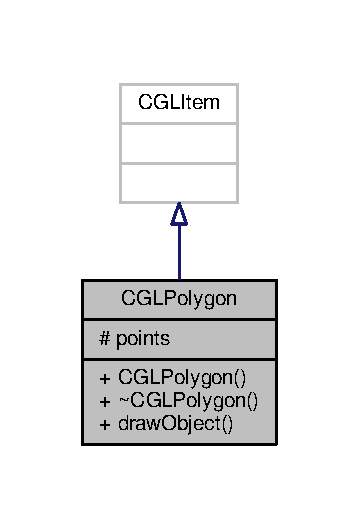
\includegraphics[width=172pt]{d9/d48/class_c_g_l_polygon__inherit__graph}
\end{center}
\end{figure}


Graphe de collaboration de C\-G\-L\-Polygon\-:
\nopagebreak
\begin{figure}[H]
\begin{center}
\leavevmode
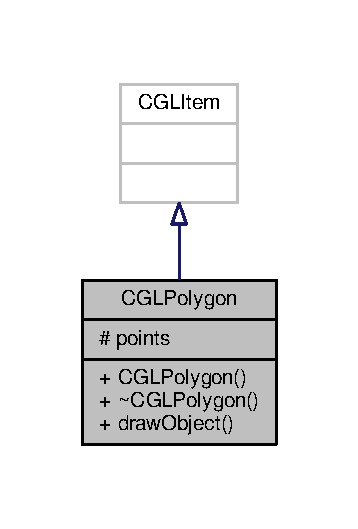
\includegraphics[width=172pt]{d0/d36/class_c_g_l_polygon__coll__graph}
\end{center}
\end{figure}
\subsection*{Fonctions membres publiques}
\begin{DoxyCompactItemize}
\item 
\hyperlink{class_c_g_l_polygon_a7727830b4fa06ad9d4fdd684d03525ab}{C\-G\-L\-Polygon} ()
\item 
virtual \hyperlink{class_c_g_l_polygon_a87b29787eaf2def21bcc61cf5cd0d76c}{$\sim$\-C\-G\-L\-Polygon} ()
\item 
void \hyperlink{class_c_g_l_polygon_a8450b134d7e40059c36ecc43133596c0}{draw\-Object} (Uint32 ellapsed\-Time)
\end{DoxyCompactItemize}
\subsection*{Attributs protégés}
\begin{DoxyCompactItemize}
\item 
list$<$ \hyperlink{class_c_g_l_vector2_d}{C\-G\-L\-Vector2\-D} $\ast$ $>$ \hyperlink{class_c_g_l_polygon_a8092f33a46cc4b79554808efa24ba025}{points}
\end{DoxyCompactItemize}


\subsection{Description détaillée}


Définition à la ligne 20 du fichier Polygon.\-h.



\subsection{Documentation des constructeurs et destructeur}
\hypertarget{class_c_g_l_polygon_a7727830b4fa06ad9d4fdd684d03525ab}{\index{C\-G\-L\-Polygon@{C\-G\-L\-Polygon}!C\-G\-L\-Polygon@{C\-G\-L\-Polygon}}
\index{C\-G\-L\-Polygon@{C\-G\-L\-Polygon}!CGLPolygon@{C\-G\-L\-Polygon}}
\subsubsection[{C\-G\-L\-Polygon}]{\setlength{\rightskip}{0pt plus 5cm}C\-G\-L\-Polygon\-::\-C\-G\-L\-Polygon (
\begin{DoxyParamCaption}
{}
\end{DoxyParamCaption}
)}}\label{class_c_g_l_polygon_a7727830b4fa06ad9d4fdd684d03525ab}


Définition à la ligne 10 du fichier Polygon.\-cpp.

\hypertarget{class_c_g_l_polygon_a87b29787eaf2def21bcc61cf5cd0d76c}{\index{C\-G\-L\-Polygon@{C\-G\-L\-Polygon}!$\sim$\-C\-G\-L\-Polygon@{$\sim$\-C\-G\-L\-Polygon}}
\index{$\sim$\-C\-G\-L\-Polygon@{$\sim$\-C\-G\-L\-Polygon}!CGLPolygon@{C\-G\-L\-Polygon}}
\subsubsection[{$\sim$\-C\-G\-L\-Polygon}]{\setlength{\rightskip}{0pt plus 5cm}C\-G\-L\-Polygon\-::$\sim$\-C\-G\-L\-Polygon (
\begin{DoxyParamCaption}
{}
\end{DoxyParamCaption}
)\hspace{0.3cm}{\ttfamily [virtual]}}}\label{class_c_g_l_polygon_a87b29787eaf2def21bcc61cf5cd0d76c}


Définition à la ligne 24 du fichier Polygon.\-cpp.



\subsection{Documentation des fonctions membres}
\hypertarget{class_c_g_l_polygon_a8450b134d7e40059c36ecc43133596c0}{\index{C\-G\-L\-Polygon@{C\-G\-L\-Polygon}!draw\-Object@{draw\-Object}}
\index{draw\-Object@{draw\-Object}!CGLPolygon@{C\-G\-L\-Polygon}}
\subsubsection[{draw\-Object}]{\setlength{\rightskip}{0pt plus 5cm}void C\-G\-L\-Polygon\-::draw\-Object (
\begin{DoxyParamCaption}
\item[{Uint32}]{ellapsed\-Time}
\end{DoxyParamCaption}
)}}\label{class_c_g_l_polygon_a8450b134d7e40059c36ecc43133596c0}


Définition à la ligne 29 du fichier Polygon.\-cpp.



\subsection{Documentation des données membres}
\hypertarget{class_c_g_l_polygon_a8092f33a46cc4b79554808efa24ba025}{\index{C\-G\-L\-Polygon@{C\-G\-L\-Polygon}!points@{points}}
\index{points@{points}!CGLPolygon@{C\-G\-L\-Polygon}}
\subsubsection[{points}]{\setlength{\rightskip}{0pt plus 5cm}list$<${\bf C\-G\-L\-Vector2\-D}$\ast$$>$ C\-G\-L\-Polygon\-::points\hspace{0.3cm}{\ttfamily [protected]}}}\label{class_c_g_l_polygon_a8092f33a46cc4b79554808efa24ba025}


Définition à la ligne 23 du fichier Polygon.\-h.



La documentation de cette classe a été générée à partir des fichiers suivants \-:\begin{DoxyCompactItemize}
\item 
/home/dagal/git/\-D\-G\-L/\-Damier\-G\-L/src/\-C\-G\-L/\hyperlink{_polygon_8h}{Polygon.\-h}\item 
/home/dagal/git/\-D\-G\-L/\-Damier\-G\-L/src/\-C\-G\-L/\hyperlink{_polygon_8cpp}{Polygon.\-cpp}\end{DoxyCompactItemize}

\hypertarget{class_c_g_l_position}{\section{Référence de la classe C\-G\-L\-Position}
\label{class_c_g_l_position}\index{C\-G\-L\-Position@{C\-G\-L\-Position}}
}


{\ttfamily \#include $<$Position.\-h$>$}



Graphe d'héritage de C\-G\-L\-Position\-:
\nopagebreak
\begin{figure}[H]
\begin{center}
\leavevmode
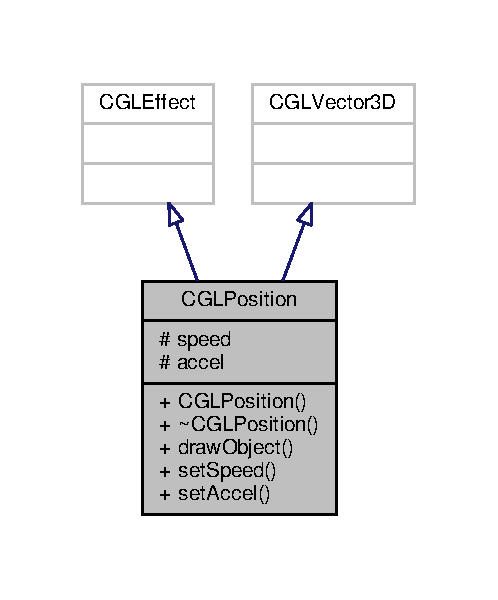
\includegraphics[width=239pt]{d7/d46/class_c_g_l_position__inherit__graph}
\end{center}
\end{figure}


Graphe de collaboration de C\-G\-L\-Position\-:
\nopagebreak
\begin{figure}[H]
\begin{center}
\leavevmode
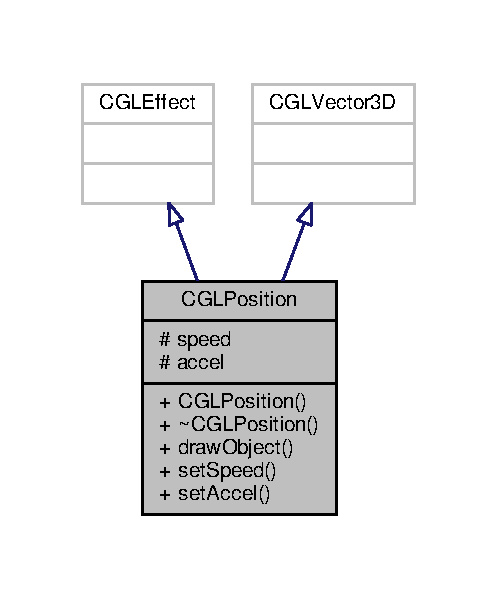
\includegraphics[width=239pt]{df/df1/class_c_g_l_position__coll__graph}
\end{center}
\end{figure}
\subsection*{Fonctions membres publiques}
\begin{DoxyCompactItemize}
\item 
\hyperlink{class_c_g_l_position_ab32bdd49fc31414e874917568e5d37d2}{C\-G\-L\-Position} ()
\item 
virtual \hyperlink{class_c_g_l_position_afe1ee045b528494d23286adf06aecae0}{$\sim$\-C\-G\-L\-Position} ()
\item 
void \hyperlink{class_c_g_l_position_a439ae873ba7ef56826a27eb7b15b0b6f}{draw\-Object} (Uint32 ellapsed\-Time)
\item 
void \hyperlink{class_c_g_l_position_a729e7b3f01b8c735d60d8c51b6610eef}{set\-Speed} (double const sx, double const sy, double const sz)
\item 
void \hyperlink{class_c_g_l_position_a5a43a8991d3d8ca645edbcfb0e97db20}{set\-Accel} (double const ax, double const ay, double const az)
\end{DoxyCompactItemize}
\subsection*{Attributs protégés}
\begin{DoxyCompactItemize}
\item 
C\-G\-L\-Vector3\-D \hyperlink{class_c_g_l_position_ac5a3b64ac5c800b84a3b621e6e50c381}{speed}
\item 
C\-G\-L\-Vector3\-D \hyperlink{class_c_g_l_position_abb7ae2f19acbbcc53d685c9ee0e948ce}{accel}
\end{DoxyCompactItemize}


\subsection{Description détaillée}


Définition à la ligne 14 du fichier Position.\-h.



\subsection{Documentation des constructeurs et destructeur}
\hypertarget{class_c_g_l_position_ab32bdd49fc31414e874917568e5d37d2}{\index{C\-G\-L\-Position@{C\-G\-L\-Position}!C\-G\-L\-Position@{C\-G\-L\-Position}}
\index{C\-G\-L\-Position@{C\-G\-L\-Position}!CGLPosition@{C\-G\-L\-Position}}
\subsubsection[{C\-G\-L\-Position}]{\setlength{\rightskip}{0pt plus 5cm}C\-G\-L\-Position\-::\-C\-G\-L\-Position (
\begin{DoxyParamCaption}
{}
\end{DoxyParamCaption}
)}}\label{class_c_g_l_position_ab32bdd49fc31414e874917568e5d37d2}


Définition à la ligne 10 du fichier Position.\-cpp.

\hypertarget{class_c_g_l_position_afe1ee045b528494d23286adf06aecae0}{\index{C\-G\-L\-Position@{C\-G\-L\-Position}!$\sim$\-C\-G\-L\-Position@{$\sim$\-C\-G\-L\-Position}}
\index{$\sim$\-C\-G\-L\-Position@{$\sim$\-C\-G\-L\-Position}!CGLPosition@{C\-G\-L\-Position}}
\subsubsection[{$\sim$\-C\-G\-L\-Position}]{\setlength{\rightskip}{0pt plus 5cm}C\-G\-L\-Position\-::$\sim$\-C\-G\-L\-Position (
\begin{DoxyParamCaption}
{}
\end{DoxyParamCaption}
)\hspace{0.3cm}{\ttfamily [virtual]}}}\label{class_c_g_l_position_afe1ee045b528494d23286adf06aecae0}


Définition à la ligne 16 du fichier Position.\-cpp.



\subsection{Documentation des fonctions membres}
\hypertarget{class_c_g_l_position_a439ae873ba7ef56826a27eb7b15b0b6f}{\index{C\-G\-L\-Position@{C\-G\-L\-Position}!draw\-Object@{draw\-Object}}
\index{draw\-Object@{draw\-Object}!CGLPosition@{C\-G\-L\-Position}}
\subsubsection[{draw\-Object}]{\setlength{\rightskip}{0pt plus 5cm}void C\-G\-L\-Position\-::draw\-Object (
\begin{DoxyParamCaption}
\item[{Uint32}]{ellapsed\-Time}
\end{DoxyParamCaption}
)}}\label{class_c_g_l_position_a439ae873ba7ef56826a27eb7b15b0b6f}


Définition à la ligne 30 du fichier Position.\-cpp.

\hypertarget{class_c_g_l_position_a5a43a8991d3d8ca645edbcfb0e97db20}{\index{C\-G\-L\-Position@{C\-G\-L\-Position}!set\-Accel@{set\-Accel}}
\index{set\-Accel@{set\-Accel}!CGLPosition@{C\-G\-L\-Position}}
\subsubsection[{set\-Accel}]{\setlength{\rightskip}{0pt plus 5cm}void C\-G\-L\-Position\-::set\-Accel (
\begin{DoxyParamCaption}
\item[{double const}]{ax, }
\item[{double const}]{ay, }
\item[{double const}]{az}
\end{DoxyParamCaption}
)}}\label{class_c_g_l_position_a5a43a8991d3d8ca645edbcfb0e97db20}


Définition à la ligne 25 du fichier Position.\-cpp.



Voici le graphe des appelants de cette fonction \-:
\nopagebreak
\begin{figure}[H]
\begin{center}
\leavevmode
\includegraphics[width=270pt]{de/d31/class_c_g_l_position_a5a43a8991d3d8ca645edbcfb0e97db20_icgraph}
\end{center}
\end{figure}


\hypertarget{class_c_g_l_position_a729e7b3f01b8c735d60d8c51b6610eef}{\index{C\-G\-L\-Position@{C\-G\-L\-Position}!set\-Speed@{set\-Speed}}
\index{set\-Speed@{set\-Speed}!CGLPosition@{C\-G\-L\-Position}}
\subsubsection[{set\-Speed}]{\setlength{\rightskip}{0pt plus 5cm}void C\-G\-L\-Position\-::set\-Speed (
\begin{DoxyParamCaption}
\item[{double const}]{sx, }
\item[{double const}]{sy, }
\item[{double const}]{sz}
\end{DoxyParamCaption}
)}}\label{class_c_g_l_position_a729e7b3f01b8c735d60d8c51b6610eef}


Définition à la ligne 20 du fichier Position.\-cpp.



Voici le graphe des appelants de cette fonction \-:
\nopagebreak
\begin{figure}[H]
\begin{center}
\leavevmode
\includegraphics[width=274pt]{de/d31/class_c_g_l_position_a729e7b3f01b8c735d60d8c51b6610eef_icgraph}
\end{center}
\end{figure}




\subsection{Documentation des données membres}
\hypertarget{class_c_g_l_position_abb7ae2f19acbbcc53d685c9ee0e948ce}{\index{C\-G\-L\-Position@{C\-G\-L\-Position}!accel@{accel}}
\index{accel@{accel}!CGLPosition@{C\-G\-L\-Position}}
\subsubsection[{accel}]{\setlength{\rightskip}{0pt plus 5cm}C\-G\-L\-Vector3\-D C\-G\-L\-Position\-::accel\hspace{0.3cm}{\ttfamily [protected]}}}\label{class_c_g_l_position_abb7ae2f19acbbcc53d685c9ee0e948ce}


Définition à la ligne 21 du fichier Position.\-h.

\hypertarget{class_c_g_l_position_ac5a3b64ac5c800b84a3b621e6e50c381}{\index{C\-G\-L\-Position@{C\-G\-L\-Position}!speed@{speed}}
\index{speed@{speed}!CGLPosition@{C\-G\-L\-Position}}
\subsubsection[{speed}]{\setlength{\rightskip}{0pt plus 5cm}C\-G\-L\-Vector3\-D C\-G\-L\-Position\-::speed\hspace{0.3cm}{\ttfamily [protected]}}}\label{class_c_g_l_position_ac5a3b64ac5c800b84a3b621e6e50c381}


Définition à la ligne 20 du fichier Position.\-h.



La documentation de cette classe a été générée à partir des fichiers suivants \-:\begin{DoxyCompactItemize}
\item 
/home/dagal/git/\-D\-G\-L/\-Damier\-G\-L/src/\-C\-G\-L/\hyperlink{_position_8h}{Position.\-h}\item 
/home/dagal/git/\-D\-G\-L/\-Damier\-G\-L/src/\-C\-G\-L/\hyperlink{_position_8cpp}{Position.\-cpp}\end{DoxyCompactItemize}

\hypertarget{class_c_g_l_quad}{\section{Référence de la classe C\-G\-L\-Quad}
\label{class_c_g_l_quad}\index{C\-G\-L\-Quad@{C\-G\-L\-Quad}}
}


{\ttfamily \#include $<$C\-G\-L\-Quad.\-h$>$}



Graphe d'héritage de C\-G\-L\-Quad\-:\nopagebreak
\begin{figure}[H]
\begin{center}
\leavevmode
\includegraphics[height=550pt]{d8/de4/class_c_g_l_quad__inherit__graph}
\end{center}
\end{figure}


Graphe de collaboration de C\-G\-L\-Quad\-:\nopagebreak
\begin{figure}[H]
\begin{center}
\leavevmode
\includegraphics[width=267pt]{dd/d46/class_c_g_l_quad__coll__graph}
\end{center}
\end{figure}
\subsection*{Fonctions membres publiques}
\begin{DoxyCompactItemize}
\item 
\hyperlink{class_c_g_l_quad_a95b07c1605f65de30cb47b65fa364294}{C\-G\-L\-Quad} ()
\item 
\hyperlink{class_c_g_l_quad_a6a78f1183a166adf08bfe3880f2cd415}{C\-G\-L\-Quad} (double x, double y, double z, double r)
\item 
virtual \hyperlink{class_c_g_l_quad_a19320cf64816de2de1fa7540acbf833e}{$\sim$\-C\-G\-L\-Quad} ()
\item 
void \hyperlink{class_c_g_l_quad_a81696d558e2355af7d621cdbf0ccf41a}{draw\-Object} (Uint32 time\-Ellapsed)
\end{DoxyCompactItemize}
\subsection*{Attributs protégés}
\begin{DoxyCompactItemize}
\item 
double \hyperlink{class_c_g_l_quad_a53dcf6352ff92cde8cc4b9756e51057e}{longueur}
\end{DoxyCompactItemize}
\subsection*{Membres hérités additionnels}


\subsection{Description détaillée}


Définition à la ligne 13 du fichier C\-G\-L\-Quad.\-h.



\subsection{Documentation des constructeurs et destructeur}
\hypertarget{class_c_g_l_quad_a95b07c1605f65de30cb47b65fa364294}{\index{C\-G\-L\-Quad@{C\-G\-L\-Quad}!C\-G\-L\-Quad@{C\-G\-L\-Quad}}
\index{C\-G\-L\-Quad@{C\-G\-L\-Quad}!CGLQuad@{C\-G\-L\-Quad}}
\subsubsection[{C\-G\-L\-Quad}]{\setlength{\rightskip}{0pt plus 5cm}C\-G\-L\-Quad\-::\-C\-G\-L\-Quad (
\begin{DoxyParamCaption}
{}
\end{DoxyParamCaption}
)}}\label{class_c_g_l_quad_a95b07c1605f65de30cb47b65fa364294}


Définition à la ligne 10 du fichier C\-G\-L\-Quad.\-cpp.

\hypertarget{class_c_g_l_quad_a6a78f1183a166adf08bfe3880f2cd415}{\index{C\-G\-L\-Quad@{C\-G\-L\-Quad}!C\-G\-L\-Quad@{C\-G\-L\-Quad}}
\index{C\-G\-L\-Quad@{C\-G\-L\-Quad}!CGLQuad@{C\-G\-L\-Quad}}
\subsubsection[{C\-G\-L\-Quad}]{\setlength{\rightskip}{0pt plus 5cm}C\-G\-L\-Quad\-::\-C\-G\-L\-Quad (
\begin{DoxyParamCaption}
\item[{double}]{x, }
\item[{double}]{y, }
\item[{double}]{z, }
\item[{double}]{r}
\end{DoxyParamCaption}
)}}\label{class_c_g_l_quad_a6a78f1183a166adf08bfe3880f2cd415}


Définition à la ligne 16 du fichier C\-G\-L\-Quad.\-cpp.

\hypertarget{class_c_g_l_quad_a19320cf64816de2de1fa7540acbf833e}{\index{C\-G\-L\-Quad@{C\-G\-L\-Quad}!$\sim$\-C\-G\-L\-Quad@{$\sim$\-C\-G\-L\-Quad}}
\index{$\sim$\-C\-G\-L\-Quad@{$\sim$\-C\-G\-L\-Quad}!CGLQuad@{C\-G\-L\-Quad}}
\subsubsection[{$\sim$\-C\-G\-L\-Quad}]{\setlength{\rightskip}{0pt plus 5cm}C\-G\-L\-Quad\-::$\sim$\-C\-G\-L\-Quad (
\begin{DoxyParamCaption}
{}
\end{DoxyParamCaption}
)\hspace{0.3cm}{\ttfamily [virtual]}}}\label{class_c_g_l_quad_a19320cf64816de2de1fa7540acbf833e}


Définition à la ligne 21 du fichier C\-G\-L\-Quad.\-cpp.



\subsection{Documentation des fonctions membres}
\hypertarget{class_c_g_l_quad_a81696d558e2355af7d621cdbf0ccf41a}{\index{C\-G\-L\-Quad@{C\-G\-L\-Quad}!draw\-Object@{draw\-Object}}
\index{draw\-Object@{draw\-Object}!CGLQuad@{C\-G\-L\-Quad}}
\subsubsection[{draw\-Object}]{\setlength{\rightskip}{0pt plus 5cm}void C\-G\-L\-Quad\-::draw\-Object (
\begin{DoxyParamCaption}
\item[{Uint32}]{time\-Ellapsed}
\end{DoxyParamCaption}
)\hspace{0.3cm}{\ttfamily [virtual]}}}\label{class_c_g_l_quad_a81696d558e2355af7d621cdbf0ccf41a}


Réimplémentée à partir de \hyperlink{class_c_g_l_object_a2781ec98c37bd209f2382c5130a365b9}{C\-G\-L\-Object}.



Définition à la ligne 25 du fichier C\-G\-L\-Quad.\-cpp.



Voici le graphe d'appel pour cette fonction \-:\nopagebreak
\begin{figure}[H]
\begin{center}
\leavevmode
\includegraphics[width=350pt]{df/d41/class_c_g_l_quad_a81696d558e2355af7d621cdbf0ccf41a_cgraph}
\end{center}
\end{figure}




\subsection{Documentation des données membres}
\hypertarget{class_c_g_l_quad_a53dcf6352ff92cde8cc4b9756e51057e}{\index{C\-G\-L\-Quad@{C\-G\-L\-Quad}!longueur@{longueur}}
\index{longueur@{longueur}!CGLQuad@{C\-G\-L\-Quad}}
\subsubsection[{longueur}]{\setlength{\rightskip}{0pt plus 5cm}double C\-G\-L\-Quad\-::longueur\hspace{0.3cm}{\ttfamily [protected]}}}\label{class_c_g_l_quad_a53dcf6352ff92cde8cc4b9756e51057e}


Définition à la ligne 18 du fichier C\-G\-L\-Quad.\-h.



La documentation de cette classe a été générée à partir des fichiers suivants \-:\begin{DoxyCompactItemize}
\item 
/home/dagal/git/\-Damier\-G\-L/\-Damier\-G\-L/src/\-C\-G\-L/\hyperlink{_c_g_l_quad_8h}{C\-G\-L\-Quad.\-h}\item 
/home/dagal/git/\-Damier\-G\-L/\-Damier\-G\-L/src/\-C\-G\-L/\hyperlink{_c_g_l_quad_8cpp}{C\-G\-L\-Quad.\-cpp}\end{DoxyCompactItemize}

\hypertarget{class_c_g_l_robot1}{\section{Référence de la classe C\-G\-L\-Robot1}
\label{class_c_g_l_robot1}\index{C\-G\-L\-Robot1@{C\-G\-L\-Robot1}}
}


{\ttfamily \#include $<$Robot1.\-h$>$}



Graphe d'héritage de C\-G\-L\-Robot1\-:
\nopagebreak
\begin{figure}[H]
\begin{center}
\leavevmode
\includegraphics[width=168pt]{d2/dcc/class_c_g_l_robot1__inherit__graph}
\end{center}
\end{figure}


Graphe de collaboration de C\-G\-L\-Robot1\-:
\nopagebreak
\begin{figure}[H]
\begin{center}
\leavevmode
\includegraphics[width=168pt]{dc/de7/class_c_g_l_robot1__coll__graph}
\end{center}
\end{figure}
\subsection*{Fonctions membres publiques}
\begin{DoxyCompactItemize}
\item 
\hyperlink{class_c_g_l_robot1_a2b8077cc29b703e31d3ec85404cd3aed}{C\-G\-L\-Robot1} ()
\item 
virtual \hyperlink{class_c_g_l_robot1_accda840d084f72fb65d243dc047abc11}{$\sim$\-C\-G\-L\-Robot1} ()
\item 
void \hyperlink{class_c_g_l_robot1_a050d7fea4097a6634ef5feef26ae7865}{draw\-Object} (Uint32 time\-Ellapsed)
\end{DoxyCompactItemize}


\subsection{Description détaillée}


Définition à la ligne 13 du fichier Robot1.\-h.



\subsection{Documentation des constructeurs et destructeur}
\hypertarget{class_c_g_l_robot1_a2b8077cc29b703e31d3ec85404cd3aed}{\index{C\-G\-L\-Robot1@{C\-G\-L\-Robot1}!C\-G\-L\-Robot1@{C\-G\-L\-Robot1}}
\index{C\-G\-L\-Robot1@{C\-G\-L\-Robot1}!CGLRobot1@{C\-G\-L\-Robot1}}
\subsubsection[{C\-G\-L\-Robot1}]{\setlength{\rightskip}{0pt plus 5cm}C\-G\-L\-Robot1\-::\-C\-G\-L\-Robot1 (
\begin{DoxyParamCaption}
{}
\end{DoxyParamCaption}
)}}\label{class_c_g_l_robot1_a2b8077cc29b703e31d3ec85404cd3aed}


Définition à la ligne 10 du fichier Robot1.\-cpp.

\hypertarget{class_c_g_l_robot1_accda840d084f72fb65d243dc047abc11}{\index{C\-G\-L\-Robot1@{C\-G\-L\-Robot1}!$\sim$\-C\-G\-L\-Robot1@{$\sim$\-C\-G\-L\-Robot1}}
\index{$\sim$\-C\-G\-L\-Robot1@{$\sim$\-C\-G\-L\-Robot1}!CGLRobot1@{C\-G\-L\-Robot1}}
\subsubsection[{$\sim$\-C\-G\-L\-Robot1}]{\setlength{\rightskip}{0pt plus 5cm}C\-G\-L\-Robot1\-::$\sim$\-C\-G\-L\-Robot1 (
\begin{DoxyParamCaption}
{}
\end{DoxyParamCaption}
)\hspace{0.3cm}{\ttfamily [virtual]}}}\label{class_c_g_l_robot1_accda840d084f72fb65d243dc047abc11}


Définition à la ligne 26 du fichier Robot1.\-cpp.



\subsection{Documentation des fonctions membres}
\hypertarget{class_c_g_l_robot1_a050d7fea4097a6634ef5feef26ae7865}{\index{C\-G\-L\-Robot1@{C\-G\-L\-Robot1}!draw\-Object@{draw\-Object}}
\index{draw\-Object@{draw\-Object}!CGLRobot1@{C\-G\-L\-Robot1}}
\subsubsection[{draw\-Object}]{\setlength{\rightskip}{0pt plus 5cm}void C\-G\-L\-Robot1\-::draw\-Object (
\begin{DoxyParamCaption}
\item[{Uint32}]{time\-Ellapsed}
\end{DoxyParamCaption}
)}}\label{class_c_g_l_robot1_a050d7fea4097a6634ef5feef26ae7865}


Définition à la ligne 30 du fichier Robot1.\-cpp.



La documentation de cette classe a été générée à partir des fichiers suivants \-:\begin{DoxyCompactItemize}
\item 
/home/dagal/git/\-D\-G\-L/\-Damier\-G\-L/src/\-C\-G\-L/\hyperlink{_robot1_8h}{Robot1.\-h}\item 
/home/dagal/git/\-D\-G\-L/\-Damier\-G\-L/src/\-C\-G\-L/\hyperlink{_robot1_8cpp}{Robot1.\-cpp}\end{DoxyCompactItemize}

\hypertarget{class_c_g_l_rotation}{\section{Référence de la classe C\-G\-L\-Rotation}
\label{class_c_g_l_rotation}\index{C\-G\-L\-Rotation@{C\-G\-L\-Rotation}}
}


{\ttfamily \#include $<$C\-G\-L\-Rotation.\-h$>$}



Graphe d'héritage de C\-G\-L\-Rotation\-:\nopagebreak
\begin{figure}[H]
\begin{center}
\leavevmode
\includegraphics[height=550pt]{d4/d97/class_c_g_l_rotation__inherit__graph}
\end{center}
\end{figure}


Graphe de collaboration de C\-G\-L\-Rotation\-:\nopagebreak
\begin{figure}[H]
\begin{center}
\leavevmode
\includegraphics[height=550pt]{d0/db1/class_c_g_l_rotation__coll__graph}
\end{center}
\end{figure}
\subsection*{Fonctions membres publiques}
\begin{DoxyCompactItemize}
\item 
\hyperlink{class_c_g_l_rotation_a00f328e9aeefa148e4bd169afc5cb959}{C\-G\-L\-Rotation} ()
\item 
virtual \hyperlink{class_c_g_l_rotation_adc90213d4008b9beb3c8e266f952a509}{$\sim$\-C\-G\-L\-Rotation} ()
\item 
void \hyperlink{class_c_g_l_rotation_a690f30f8f121b27ac22d6b02a6443b58}{set\-A} (double av)
\item 
double \hyperlink{class_c_g_l_rotation_a0d836220b7b39ee00173ee4e0bb4da92}{get\-A} ()
\item 
void \hyperlink{class_c_g_l_rotation_a2b767e088f36ceef91e7259c76f7390e}{set} (double av, double ax, double ay, double az)
\item 
void \hyperlink{class_c_g_l_rotation_a94be2c089fbe52d0f8cb33ee98f8de74}{draw\-Object} (Uint32 ellapsed\-Time)
\end{DoxyCompactItemize}
\subsection*{Membres hérités additionnels}


\subsection{Description détaillée}


Définition à la ligne 17 du fichier C\-G\-L\-Rotation.\-h.



\subsection{Documentation des constructeurs et destructeur}
\hypertarget{class_c_g_l_rotation_a00f328e9aeefa148e4bd169afc5cb959}{\index{C\-G\-L\-Rotation@{C\-G\-L\-Rotation}!C\-G\-L\-Rotation@{C\-G\-L\-Rotation}}
\index{C\-G\-L\-Rotation@{C\-G\-L\-Rotation}!CGLRotation@{C\-G\-L\-Rotation}}
\subsubsection[{C\-G\-L\-Rotation}]{\setlength{\rightskip}{0pt plus 5cm}C\-G\-L\-Rotation\-::\-C\-G\-L\-Rotation (
\begin{DoxyParamCaption}
{}
\end{DoxyParamCaption}
)}}\label{class_c_g_l_rotation_a00f328e9aeefa148e4bd169afc5cb959}


Définition à la ligne 10 du fichier C\-G\-L\-Rotation.\-cpp.

\hypertarget{class_c_g_l_rotation_adc90213d4008b9beb3c8e266f952a509}{\index{C\-G\-L\-Rotation@{C\-G\-L\-Rotation}!$\sim$\-C\-G\-L\-Rotation@{$\sim$\-C\-G\-L\-Rotation}}
\index{$\sim$\-C\-G\-L\-Rotation@{$\sim$\-C\-G\-L\-Rotation}!CGLRotation@{C\-G\-L\-Rotation}}
\subsubsection[{$\sim$\-C\-G\-L\-Rotation}]{\setlength{\rightskip}{0pt plus 5cm}C\-G\-L\-Rotation\-::$\sim$\-C\-G\-L\-Rotation (
\begin{DoxyParamCaption}
{}
\end{DoxyParamCaption}
)\hspace{0.3cm}{\ttfamily [virtual]}}}\label{class_c_g_l_rotation_adc90213d4008b9beb3c8e266f952a509}


Définition à la ligne 16 du fichier C\-G\-L\-Rotation.\-cpp.



\subsection{Documentation des fonctions membres}
\hypertarget{class_c_g_l_rotation_a94be2c089fbe52d0f8cb33ee98f8de74}{\index{C\-G\-L\-Rotation@{C\-G\-L\-Rotation}!draw\-Object@{draw\-Object}}
\index{draw\-Object@{draw\-Object}!CGLRotation@{C\-G\-L\-Rotation}}
\subsubsection[{draw\-Object}]{\setlength{\rightskip}{0pt plus 5cm}void C\-G\-L\-Rotation\-::draw\-Object (
\begin{DoxyParamCaption}
\item[{Uint32}]{ellapsed\-Time}
\end{DoxyParamCaption}
)\hspace{0.3cm}{\ttfamily [virtual]}}}\label{class_c_g_l_rotation_a94be2c089fbe52d0f8cb33ee98f8de74}


Réimplémentée à partir de \hyperlink{class_c_g_l_object_a2781ec98c37bd209f2382c5130a365b9}{C\-G\-L\-Object}.



Définition à la ligne 38 du fichier C\-G\-L\-Rotation.\-cpp.

\hypertarget{class_c_g_l_rotation_a0d836220b7b39ee00173ee4e0bb4da92}{\index{C\-G\-L\-Rotation@{C\-G\-L\-Rotation}!get\-A@{get\-A}}
\index{get\-A@{get\-A}!CGLRotation@{C\-G\-L\-Rotation}}
\subsubsection[{get\-A}]{\setlength{\rightskip}{0pt plus 5cm}double C\-G\-L\-Rotation\-::get\-A (
\begin{DoxyParamCaption}
{}
\end{DoxyParamCaption}
)}}\label{class_c_g_l_rotation_a0d836220b7b39ee00173ee4e0bb4da92}


Définition à la ligne 25 du fichier C\-G\-L\-Rotation.\-cpp.

\hypertarget{class_c_g_l_rotation_a2b767e088f36ceef91e7259c76f7390e}{\index{C\-G\-L\-Rotation@{C\-G\-L\-Rotation}!set@{set}}
\index{set@{set}!CGLRotation@{C\-G\-L\-Rotation}}
\subsubsection[{set}]{\setlength{\rightskip}{0pt plus 5cm}void C\-G\-L\-Rotation\-::set (
\begin{DoxyParamCaption}
\item[{double}]{av, }
\item[{double}]{ax, }
\item[{double}]{ay, }
\item[{double}]{az}
\end{DoxyParamCaption}
)}}\label{class_c_g_l_rotation_a2b767e088f36ceef91e7259c76f7390e}


Définition à la ligne 30 du fichier C\-G\-L\-Rotation.\-cpp.



Voici le graphe des appelants de cette fonction \-:\nopagebreak
\begin{figure}[H]
\begin{center}
\leavevmode
\includegraphics[width=248pt]{d4/dd5/class_c_g_l_rotation_a2b767e088f36ceef91e7259c76f7390e_icgraph}
\end{center}
\end{figure}


\hypertarget{class_c_g_l_rotation_a690f30f8f121b27ac22d6b02a6443b58}{\index{C\-G\-L\-Rotation@{C\-G\-L\-Rotation}!set\-A@{set\-A}}
\index{set\-A@{set\-A}!CGLRotation@{C\-G\-L\-Rotation}}
\subsubsection[{set\-A}]{\setlength{\rightskip}{0pt plus 5cm}void C\-G\-L\-Rotation\-::set\-A (
\begin{DoxyParamCaption}
\item[{double}]{av}
\end{DoxyParamCaption}
)}}\label{class_c_g_l_rotation_a690f30f8f121b27ac22d6b02a6443b58}


Définition à la ligne 20 du fichier C\-G\-L\-Rotation.\-cpp.



La documentation de cette classe a été générée à partir des fichiers suivants \-:\begin{DoxyCompactItemize}
\item 
/home/dagal/git/\-Damier\-G\-L/\-Damier\-G\-L/src/\-C\-G\-L/\hyperlink{_c_g_l_rotation_8h}{C\-G\-L\-Rotation.\-h}\item 
/home/dagal/git/\-Damier\-G\-L/\-Damier\-G\-L/src/\-C\-G\-L/\hyperlink{_c_g_l_rotation_8cpp}{C\-G\-L\-Rotation.\-cpp}\end{DoxyCompactItemize}

\hypertarget{class_c_g_l_rotation_speed}{\section{Référence de la classe C\-G\-L\-Rotation\-Speed}
\label{class_c_g_l_rotation_speed}\index{C\-G\-L\-Rotation\-Speed@{C\-G\-L\-Rotation\-Speed}}
}


{\ttfamily \#include $<$C\-G\-L\-Rotation\-Speed.\-h$>$}



Graphe d'héritage de C\-G\-L\-Rotation\-Speed\-:
\nopagebreak
\begin{figure}[H]
\begin{center}
\leavevmode
\includegraphics[height=550pt]{d0/dbb/class_c_g_l_rotation_speed__inherit__graph}
\end{center}
\end{figure}


Graphe de collaboration de C\-G\-L\-Rotation\-Speed\-:
\nopagebreak
\begin{figure}[H]
\begin{center}
\leavevmode
\includegraphics[height=550pt]{d1/dfb/class_c_g_l_rotation_speed__coll__graph}
\end{center}
\end{figure}
\subsection*{Fonctions membres publiques}
\begin{DoxyCompactItemize}
\item 
\hyperlink{class_c_g_l_rotation_speed_a6aed31b80ba1f7e050500469bf62e588}{C\-G\-L\-Rotation\-Speed} ()
\item 
virtual \hyperlink{class_c_g_l_rotation_speed_a7648604709da051825044630da6db987}{$\sim$\-C\-G\-L\-Rotation\-Speed} ()
\item 
void \hyperlink{class_c_g_l_rotation_speed_a6549d856fc0ad620fd1507744104797f}{draw\-Object} (Uint32 ellapsed\-Time)
\end{DoxyCompactItemize}
\subsection*{Attributs protégés}
\begin{DoxyCompactItemize}
\item 
double \hyperlink{class_c_g_l_rotation_speed_a5e9f478c8a0d828dac0ddee6777b45c4}{speed}
\end{DoxyCompactItemize}
\subsection*{Membres hérités additionnels}


\subsection{Description détaillée}


Définition à la ligne 17 du fichier C\-G\-L\-Rotation\-Speed.\-h.



\subsection{Documentation des constructeurs et destructeur}
\hypertarget{class_c_g_l_rotation_speed_a6aed31b80ba1f7e050500469bf62e588}{\index{C\-G\-L\-Rotation\-Speed@{C\-G\-L\-Rotation\-Speed}!C\-G\-L\-Rotation\-Speed@{C\-G\-L\-Rotation\-Speed}}
\index{C\-G\-L\-Rotation\-Speed@{C\-G\-L\-Rotation\-Speed}!CGLRotationSpeed@{C\-G\-L\-Rotation\-Speed}}
\subsubsection[{C\-G\-L\-Rotation\-Speed}]{\setlength{\rightskip}{0pt plus 5cm}C\-G\-L\-Rotation\-Speed\-::\-C\-G\-L\-Rotation\-Speed (
\begin{DoxyParamCaption}
{}
\end{DoxyParamCaption}
)}}\label{class_c_g_l_rotation_speed_a6aed31b80ba1f7e050500469bf62e588}


Définition à la ligne 10 du fichier C\-G\-L\-Rotation\-Speed.\-cpp.

\hypertarget{class_c_g_l_rotation_speed_a7648604709da051825044630da6db987}{\index{C\-G\-L\-Rotation\-Speed@{C\-G\-L\-Rotation\-Speed}!$\sim$\-C\-G\-L\-Rotation\-Speed@{$\sim$\-C\-G\-L\-Rotation\-Speed}}
\index{$\sim$\-C\-G\-L\-Rotation\-Speed@{$\sim$\-C\-G\-L\-Rotation\-Speed}!CGLRotationSpeed@{C\-G\-L\-Rotation\-Speed}}
\subsubsection[{$\sim$\-C\-G\-L\-Rotation\-Speed}]{\setlength{\rightskip}{0pt plus 5cm}C\-G\-L\-Rotation\-Speed\-::$\sim$\-C\-G\-L\-Rotation\-Speed (
\begin{DoxyParamCaption}
{}
\end{DoxyParamCaption}
)\hspace{0.3cm}{\ttfamily [virtual]}}}\label{class_c_g_l_rotation_speed_a7648604709da051825044630da6db987}


Définition à la ligne 14 du fichier C\-G\-L\-Rotation\-Speed.\-cpp.



\subsection{Documentation des fonctions membres}
\hypertarget{class_c_g_l_rotation_speed_a6549d856fc0ad620fd1507744104797f}{\index{C\-G\-L\-Rotation\-Speed@{C\-G\-L\-Rotation\-Speed}!draw\-Object@{draw\-Object}}
\index{draw\-Object@{draw\-Object}!CGLRotationSpeed@{C\-G\-L\-Rotation\-Speed}}
\subsubsection[{draw\-Object}]{\setlength{\rightskip}{0pt plus 5cm}void C\-G\-L\-Rotation\-Speed\-::draw\-Object (
\begin{DoxyParamCaption}
\item[{Uint32}]{ellapsed\-Time}
\end{DoxyParamCaption}
)\hspace{0.3cm}{\ttfamily [virtual]}}}\label{class_c_g_l_rotation_speed_a6549d856fc0ad620fd1507744104797f}


Réimplémentée à partir de \hyperlink{class_c_g_l_rotation_a94be2c089fbe52d0f8cb33ee98f8de74}{C\-G\-L\-Rotation}.



Définition à la ligne 18 du fichier C\-G\-L\-Rotation\-Speed.\-cpp.



Voici le graphe d'appel pour cette fonction \-:
\nopagebreak
\begin{figure}[H]
\begin{center}
\leavevmode
\includegraphics[width=350pt]{d4/d9e/class_c_g_l_rotation_speed_a6549d856fc0ad620fd1507744104797f_cgraph}
\end{center}
\end{figure}




\subsection{Documentation des données membres}
\hypertarget{class_c_g_l_rotation_speed_a5e9f478c8a0d828dac0ddee6777b45c4}{\index{C\-G\-L\-Rotation\-Speed@{C\-G\-L\-Rotation\-Speed}!speed@{speed}}
\index{speed@{speed}!CGLRotationSpeed@{C\-G\-L\-Rotation\-Speed}}
\subsubsection[{speed}]{\setlength{\rightskip}{0pt plus 5cm}double C\-G\-L\-Rotation\-Speed\-::speed\hspace{0.3cm}{\ttfamily [protected]}}}\label{class_c_g_l_rotation_speed_a5e9f478c8a0d828dac0ddee6777b45c4}


Définition à la ligne 20 du fichier C\-G\-L\-Rotation\-Speed.\-h.



La documentation de cette classe a été générée à partir des fichiers suivants \-:\begin{DoxyCompactItemize}
\item 
/home/dagal/git/\-Damier\-G\-L/\-Damier\-G\-L/src/\-C\-G\-L/\hyperlink{_c_g_l_rotation_speed_8h}{C\-G\-L\-Rotation\-Speed.\-h}\item 
/home/dagal/git/\-Damier\-G\-L/\-Damier\-G\-L/src/\-C\-G\-L/\hyperlink{_c_g_l_rotation_speed_8cpp}{C\-G\-L\-Rotation\-Speed.\-cpp}\end{DoxyCompactItemize}

\hypertarget{class_c_g_l_scale}{\section{Référence de la classe C\-G\-L\-Scale}
\label{class_c_g_l_scale}\index{C\-G\-L\-Scale@{C\-G\-L\-Scale}}
}


{\ttfamily \#include $<$C\-G\-L\-Scale.\-h$>$}



Graphe d'héritage de C\-G\-L\-Scale\-:
\nopagebreak
\begin{figure}[H]
\begin{center}
\leavevmode
\includegraphics[height=550pt]{d9/d69/class_c_g_l_scale__inherit__graph}
\end{center}
\end{figure}


Graphe de collaboration de C\-G\-L\-Scale\-:
\nopagebreak
\begin{figure}[H]
\begin{center}
\leavevmode
\includegraphics[width=350pt]{dd/d3a/class_c_g_l_scale__coll__graph}
\end{center}
\end{figure}
\subsection*{Fonctions membres publiques}
\begin{DoxyCompactItemize}
\item 
\hyperlink{class_c_g_l_scale_a48ed3886215e1ee3ae43fedae36cf426}{C\-G\-L\-Scale} ()
\item 
virtual \hyperlink{class_c_g_l_scale_a8a084fe6407bc5226723dd6300089cce}{$\sim$\-C\-G\-L\-Scale} ()
\item 
void \hyperlink{class_c_g_l_scale_a27939db2fb5f900800f391bb06a387a4}{draw\-Object} (Uint32 ellapsed\-Time)
\end{DoxyCompactItemize}
\subsection*{Membres hérités additionnels}


\subsection{Description détaillée}


Définition à la ligne 17 du fichier C\-G\-L\-Scale.\-h.



\subsection{Documentation des constructeurs et destructeur}
\hypertarget{class_c_g_l_scale_a48ed3886215e1ee3ae43fedae36cf426}{\index{C\-G\-L\-Scale@{C\-G\-L\-Scale}!C\-G\-L\-Scale@{C\-G\-L\-Scale}}
\index{C\-G\-L\-Scale@{C\-G\-L\-Scale}!CGLScale@{C\-G\-L\-Scale}}
\subsubsection[{C\-G\-L\-Scale}]{\setlength{\rightskip}{0pt plus 5cm}C\-G\-L\-Scale\-::\-C\-G\-L\-Scale (
\begin{DoxyParamCaption}
{}
\end{DoxyParamCaption}
)}}\label{class_c_g_l_scale_a48ed3886215e1ee3ae43fedae36cf426}


Définition à la ligne 10 du fichier C\-G\-L\-Scale.\-cpp.

\hypertarget{class_c_g_l_scale_a8a084fe6407bc5226723dd6300089cce}{\index{C\-G\-L\-Scale@{C\-G\-L\-Scale}!$\sim$\-C\-G\-L\-Scale@{$\sim$\-C\-G\-L\-Scale}}
\index{$\sim$\-C\-G\-L\-Scale@{$\sim$\-C\-G\-L\-Scale}!CGLScale@{C\-G\-L\-Scale}}
\subsubsection[{$\sim$\-C\-G\-L\-Scale}]{\setlength{\rightskip}{0pt plus 5cm}C\-G\-L\-Scale\-::$\sim$\-C\-G\-L\-Scale (
\begin{DoxyParamCaption}
{}
\end{DoxyParamCaption}
)\hspace{0.3cm}{\ttfamily [virtual]}}}\label{class_c_g_l_scale_a8a084fe6407bc5226723dd6300089cce}


Définition à la ligne 15 du fichier C\-G\-L\-Scale.\-cpp.



\subsection{Documentation des fonctions membres}
\hypertarget{class_c_g_l_scale_a27939db2fb5f900800f391bb06a387a4}{\index{C\-G\-L\-Scale@{C\-G\-L\-Scale}!draw\-Object@{draw\-Object}}
\index{draw\-Object@{draw\-Object}!CGLScale@{C\-G\-L\-Scale}}
\subsubsection[{draw\-Object}]{\setlength{\rightskip}{0pt plus 5cm}void C\-G\-L\-Scale\-::draw\-Object (
\begin{DoxyParamCaption}
\item[{Uint32}]{ellapsed\-Time}
\end{DoxyParamCaption}
)\hspace{0.3cm}{\ttfamily [virtual]}}}\label{class_c_g_l_scale_a27939db2fb5f900800f391bb06a387a4}


Réimplémentée à partir de \hyperlink{class_c_g_l_object_a2781ec98c37bd209f2382c5130a365b9}{C\-G\-L\-Object}.



Définition à la ligne 19 du fichier C\-G\-L\-Scale.\-cpp.



La documentation de cette classe a été générée à partir des fichiers suivants \-:\begin{DoxyCompactItemize}
\item 
/home/dagal/git/\-Damier\-G\-L/\-Damier\-G\-L/src/\-C\-G\-L/\hyperlink{_c_g_l_scale_8h}{C\-G\-L\-Scale.\-h}\item 
/home/dagal/git/\-Damier\-G\-L/\-Damier\-G\-L/src/\-C\-G\-L/\hyperlink{_c_g_l_scale_8cpp}{C\-G\-L\-Scale.\-cpp}\end{DoxyCompactItemize}

\hypertarget{class_c_g_l_scene}{\section{Référence de la classe C\-G\-L\-Scene}
\label{class_c_g_l_scene}\index{C\-G\-L\-Scene@{C\-G\-L\-Scene}}
}


{\ttfamily \#include $<$C\-G\-L\-Scene.\-h$>$}



Graphe d'héritage de C\-G\-L\-Scene\-:\nopagebreak
\begin{figure}[H]
\begin{center}
\leavevmode
\includegraphics[height=550pt]{dd/d28/class_c_g_l_scene__inherit__graph}
\end{center}
\end{figure}


Graphe de collaboration de C\-G\-L\-Scene\-:\nopagebreak
\begin{figure}[H]
\begin{center}
\leavevmode
\includegraphics[height=550pt]{d1/ddc/class_c_g_l_scene__coll__graph}
\end{center}
\end{figure}
\subsection*{Fonctions membres publiques}
\begin{DoxyCompactItemize}
\item 
\hyperlink{class_c_g_l_scene_aa221e551bb267aca47c05cbb3121ccb6}{C\-G\-L\-Scene} ()
\item 
virtual \hyperlink{class_c_g_l_scene_a5436d6d4aab37ec1940ce16df0fe97b8}{$\sim$\-C\-G\-L\-Scene} ()
\item 
void \hyperlink{class_c_g_l_scene_ad6c70504f83937f819d08e76d25f05d0}{draw} (Uint32 time\-Ellapsed)
\item 
\hyperlink{class_c_g_l_camera}{C\-G\-L\-Camera} $\ast$ \hyperlink{class_c_g_l_scene_afa2e2794f2f8c6b80b293703e411f7fe}{get\-Current\-Camera} ()
\item 
void \hyperlink{class_c_g_l_scene_acb982aaf33d81d1169a0a7844ac2ee6a}{add\-Camera} (\hyperlink{class_c_g_l_camera}{C\-G\-L\-Camera} $\ast$cam)
\item 
void \hyperlink{class_c_g_l_scene_aca6d85a7e345751c7fa58ca68bde3ea2}{add\-Item} (\hyperlink{class_c_g_l_object}{C\-G\-L\-Object} $\ast$obj)
\end{DoxyCompactItemize}
\subsection*{Attributs protégés}
\begin{DoxyCompactItemize}
\item 
\hyperlink{class_c_g_l_camera_list}{C\-G\-L\-Camera\-List} $\ast$ \hyperlink{class_c_g_l_scene_aa57c4220c940450c378279aaf35ef336}{cameras}
\item 
\hyperlink{class_c_g_l_object}{C\-G\-L\-Object} $\ast$ \hyperlink{class_c_g_l_scene_a4663f82695310eb9bee34ecc1c74c886}{objects}
\end{DoxyCompactItemize}
\subsection*{Membres hérités additionnels}


\subsection{Description détaillée}


Définition à la ligne 16 du fichier C\-G\-L\-Scene.\-h.



\subsection{Documentation des constructeurs et destructeur}
\hypertarget{class_c_g_l_scene_aa221e551bb267aca47c05cbb3121ccb6}{\index{C\-G\-L\-Scene@{C\-G\-L\-Scene}!C\-G\-L\-Scene@{C\-G\-L\-Scene}}
\index{C\-G\-L\-Scene@{C\-G\-L\-Scene}!CGLScene@{C\-G\-L\-Scene}}
\subsubsection[{C\-G\-L\-Scene}]{\setlength{\rightskip}{0pt plus 5cm}C\-G\-L\-Scene\-::\-C\-G\-L\-Scene (
\begin{DoxyParamCaption}
{}
\end{DoxyParamCaption}
)}}\label{class_c_g_l_scene_aa221e551bb267aca47c05cbb3121ccb6}


Définition à la ligne 11 du fichier C\-G\-L\-Scene.\-cpp.



Voici le graphe d'appel pour cette fonction \-:\nopagebreak
\begin{figure}[H]
\begin{center}
\leavevmode
\includegraphics[width=350pt]{d9/d85/class_c_g_l_scene_aa221e551bb267aca47c05cbb3121ccb6_cgraph}
\end{center}
\end{figure}


\hypertarget{class_c_g_l_scene_a5436d6d4aab37ec1940ce16df0fe97b8}{\index{C\-G\-L\-Scene@{C\-G\-L\-Scene}!$\sim$\-C\-G\-L\-Scene@{$\sim$\-C\-G\-L\-Scene}}
\index{$\sim$\-C\-G\-L\-Scene@{$\sim$\-C\-G\-L\-Scene}!CGLScene@{C\-G\-L\-Scene}}
\subsubsection[{$\sim$\-C\-G\-L\-Scene}]{\setlength{\rightskip}{0pt plus 5cm}C\-G\-L\-Scene\-::$\sim$\-C\-G\-L\-Scene (
\begin{DoxyParamCaption}
{}
\end{DoxyParamCaption}
)\hspace{0.3cm}{\ttfamily [virtual]}}}\label{class_c_g_l_scene_a5436d6d4aab37ec1940ce16df0fe97b8}


Définition à la ligne 37 du fichier C\-G\-L\-Scene.\-cpp.



\subsection{Documentation des fonctions membres}
\hypertarget{class_c_g_l_scene_acb982aaf33d81d1169a0a7844ac2ee6a}{\index{C\-G\-L\-Scene@{C\-G\-L\-Scene}!add\-Camera@{add\-Camera}}
\index{add\-Camera@{add\-Camera}!CGLScene@{C\-G\-L\-Scene}}
\subsubsection[{add\-Camera}]{\setlength{\rightskip}{0pt plus 5cm}void C\-G\-L\-Scene\-::add\-Camera (
\begin{DoxyParamCaption}
\item[{{\bf C\-G\-L\-Camera} $\ast$}]{cam}
\end{DoxyParamCaption}
)}}\label{class_c_g_l_scene_acb982aaf33d81d1169a0a7844ac2ee6a}


Définition à la ligne 54 du fichier C\-G\-L\-Scene.\-cpp.



Voici le graphe d'appel pour cette fonction \-:\nopagebreak
\begin{figure}[H]
\begin{center}
\leavevmode
\includegraphics[width=350pt]{d9/d85/class_c_g_l_scene_acb982aaf33d81d1169a0a7844ac2ee6a_cgraph}
\end{center}
\end{figure}


\hypertarget{class_c_g_l_scene_aca6d85a7e345751c7fa58ca68bde3ea2}{\index{C\-G\-L\-Scene@{C\-G\-L\-Scene}!add\-Item@{add\-Item}}
\index{add\-Item@{add\-Item}!CGLScene@{C\-G\-L\-Scene}}
\subsubsection[{add\-Item}]{\setlength{\rightskip}{0pt plus 5cm}void C\-G\-L\-Scene\-::add\-Item (
\begin{DoxyParamCaption}
\item[{{\bf C\-G\-L\-Object} $\ast$}]{obj}
\end{DoxyParamCaption}
)}}\label{class_c_g_l_scene_aca6d85a7e345751c7fa58ca68bde3ea2}


Définition à la ligne 59 du fichier C\-G\-L\-Scene.\-cpp.



Voici le graphe d'appel pour cette fonction \-:\nopagebreak
\begin{figure}[H]
\begin{center}
\leavevmode
\includegraphics[width=350pt]{d9/d85/class_c_g_l_scene_aca6d85a7e345751c7fa58ca68bde3ea2_cgraph}
\end{center}
\end{figure}




Voici le graphe des appelants de cette fonction \-:\nopagebreak
\begin{figure}[H]
\begin{center}
\leavevmode
\includegraphics[width=260pt]{d9/d85/class_c_g_l_scene_aca6d85a7e345751c7fa58ca68bde3ea2_icgraph}
\end{center}
\end{figure}


\hypertarget{class_c_g_l_scene_ad6c70504f83937f819d08e76d25f05d0}{\index{C\-G\-L\-Scene@{C\-G\-L\-Scene}!draw@{draw}}
\index{draw@{draw}!CGLScene@{C\-G\-L\-Scene}}
\subsubsection[{draw}]{\setlength{\rightskip}{0pt plus 5cm}void C\-G\-L\-Scene\-::draw (
\begin{DoxyParamCaption}
\item[{Uint32}]{time\-Ellapsed}
\end{DoxyParamCaption}
)}}\label{class_c_g_l_scene_ad6c70504f83937f819d08e76d25f05d0}


Définition à la ligne 41 du fichier C\-G\-L\-Scene.\-cpp.



Voici le graphe d'appel pour cette fonction \-:\nopagebreak
\begin{figure}[H]
\begin{center}
\leavevmode
\includegraphics[width=350pt]{d9/d85/class_c_g_l_scene_ad6c70504f83937f819d08e76d25f05d0_cgraph}
\end{center}
\end{figure}


\hypertarget{class_c_g_l_scene_afa2e2794f2f8c6b80b293703e411f7fe}{\index{C\-G\-L\-Scene@{C\-G\-L\-Scene}!get\-Current\-Camera@{get\-Current\-Camera}}
\index{get\-Current\-Camera@{get\-Current\-Camera}!CGLScene@{C\-G\-L\-Scene}}
\subsubsection[{get\-Current\-Camera}]{\setlength{\rightskip}{0pt plus 5cm}{\bf C\-G\-L\-Camera} $\ast$ C\-G\-L\-Scene\-::get\-Current\-Camera (
\begin{DoxyParamCaption}
{}
\end{DoxyParamCaption}
)}}\label{class_c_g_l_scene_afa2e2794f2f8c6b80b293703e411f7fe}


Définition à la ligne 48 du fichier C\-G\-L\-Scene.\-cpp.



Voici le graphe d'appel pour cette fonction \-:\nopagebreak
\begin{figure}[H]
\begin{center}
\leavevmode
\includegraphics[width=350pt]{d9/d85/class_c_g_l_scene_afa2e2794f2f8c6b80b293703e411f7fe_cgraph}
\end{center}
\end{figure}




Voici le graphe des appelants de cette fonction \-:\nopagebreak
\begin{figure}[H]
\begin{center}
\leavevmode
\includegraphics[width=350pt]{d9/d85/class_c_g_l_scene_afa2e2794f2f8c6b80b293703e411f7fe_icgraph}
\end{center}
\end{figure}




\subsection{Documentation des données membres}
\hypertarget{class_c_g_l_scene_aa57c4220c940450c378279aaf35ef336}{\index{C\-G\-L\-Scene@{C\-G\-L\-Scene}!cameras@{cameras}}
\index{cameras@{cameras}!CGLScene@{C\-G\-L\-Scene}}
\subsubsection[{cameras}]{\setlength{\rightskip}{0pt plus 5cm}{\bf C\-G\-L\-Camera\-List}$\ast$ C\-G\-L\-Scene\-::cameras\hspace{0.3cm}{\ttfamily [protected]}}}\label{class_c_g_l_scene_aa57c4220c940450c378279aaf35ef336}


Définition à la ligne 22 du fichier C\-G\-L\-Scene.\-h.

\hypertarget{class_c_g_l_scene_a4663f82695310eb9bee34ecc1c74c886}{\index{C\-G\-L\-Scene@{C\-G\-L\-Scene}!objects@{objects}}
\index{objects@{objects}!CGLScene@{C\-G\-L\-Scene}}
\subsubsection[{objects}]{\setlength{\rightskip}{0pt plus 5cm}{\bf C\-G\-L\-Object}$\ast$ C\-G\-L\-Scene\-::objects\hspace{0.3cm}{\ttfamily [protected]}}}\label{class_c_g_l_scene_a4663f82695310eb9bee34ecc1c74c886}


Définition à la ligne 23 du fichier C\-G\-L\-Scene.\-h.



La documentation de cette classe a été générée à partir des fichiers suivants \-:\begin{DoxyCompactItemize}
\item 
/home/dagal/git/\-Damier\-G\-L/\-Damier\-G\-L/src/\-C\-G\-L/\hyperlink{_c_g_l_scene_8h}{C\-G\-L\-Scene.\-h}\item 
/home/dagal/git/\-Damier\-G\-L/\-Damier\-G\-L/src/\-C\-G\-L/\hyperlink{_c_g_l_scene_8cpp}{C\-G\-L\-Scene.\-cpp}\end{DoxyCompactItemize}

\hypertarget{class_c_g_l_special}{\section{Référence de la classe C\-G\-L\-Special}
\label{class_c_g_l_special}\index{C\-G\-L\-Special@{C\-G\-L\-Special}}
}


{\ttfamily \#include $<$C\-G\-L\-Special.\-h$>$}



Graphe d'héritage de C\-G\-L\-Special\-:\nopagebreak
\begin{figure}[H]
\begin{center}
\leavevmode
\includegraphics[width=350pt]{d6/d0c/class_c_g_l_special__inherit__graph}
\end{center}
\end{figure}


Graphe de collaboration de C\-G\-L\-Special\-:\nopagebreak
\begin{figure}[H]
\begin{center}
\leavevmode
\includegraphics[width=267pt]{d1/d9f/class_c_g_l_special__coll__graph}
\end{center}
\end{figure}
\subsection*{Fonctions membres publiques}
\begin{DoxyCompactItemize}
\item 
\hyperlink{class_c_g_l_special_a897ae06287f83628c5d3af05135f05f1}{C\-G\-L\-Special} ()
\item 
virtual \hyperlink{class_c_g_l_special_a73dcc1a3cc05683f0fe8640aa219b68c}{$\sim$\-C\-G\-L\-Special} ()
\end{DoxyCompactItemize}
\subsection*{Membres hérités additionnels}


\subsection{Description détaillée}


Définition à la ligne 17 du fichier C\-G\-L\-Special.\-h.



\subsection{Documentation des constructeurs et destructeur}
\hypertarget{class_c_g_l_special_a897ae06287f83628c5d3af05135f05f1}{\index{C\-G\-L\-Special@{C\-G\-L\-Special}!C\-G\-L\-Special@{C\-G\-L\-Special}}
\index{C\-G\-L\-Special@{C\-G\-L\-Special}!CGLSpecial@{C\-G\-L\-Special}}
\subsubsection[{C\-G\-L\-Special}]{\setlength{\rightskip}{0pt plus 5cm}C\-G\-L\-Special\-::\-C\-G\-L\-Special (
\begin{DoxyParamCaption}
{}
\end{DoxyParamCaption}
)}}\label{class_c_g_l_special_a897ae06287f83628c5d3af05135f05f1}


Définition à la ligne 10 du fichier C\-G\-L\-Special.\-cpp.

\hypertarget{class_c_g_l_special_a73dcc1a3cc05683f0fe8640aa219b68c}{\index{C\-G\-L\-Special@{C\-G\-L\-Special}!$\sim$\-C\-G\-L\-Special@{$\sim$\-C\-G\-L\-Special}}
\index{$\sim$\-C\-G\-L\-Special@{$\sim$\-C\-G\-L\-Special}!CGLSpecial@{C\-G\-L\-Special}}
\subsubsection[{$\sim$\-C\-G\-L\-Special}]{\setlength{\rightskip}{0pt plus 5cm}C\-G\-L\-Special\-::$\sim$\-C\-G\-L\-Special (
\begin{DoxyParamCaption}
{}
\end{DoxyParamCaption}
)\hspace{0.3cm}{\ttfamily [virtual]}}}\label{class_c_g_l_special_a73dcc1a3cc05683f0fe8640aa219b68c}


Définition à la ligne 15 du fichier C\-G\-L\-Special.\-cpp.



La documentation de cette classe a été générée à partir des fichiers suivants \-:\begin{DoxyCompactItemize}
\item 
/home/dagal/git/\-Damier\-G\-L/\-Damier\-G\-L/src/\-C\-G\-L/\hyperlink{_c_g_l_special_8h}{C\-G\-L\-Special.\-h}\item 
/home/dagal/git/\-Damier\-G\-L/\-Damier\-G\-L/src/\-C\-G\-L/\hyperlink{_c_g_l_special_8cpp}{C\-G\-L\-Special.\-cpp}\end{DoxyCompactItemize}

\hypertarget{class_c_g_l_triangle}{\section{Référence de la classe C\-G\-L\-Triangle}
\label{class_c_g_l_triangle}\index{C\-G\-L\-Triangle@{C\-G\-L\-Triangle}}
}


{\ttfamily \#include $<$C\-G\-L\-Triangle.\-h$>$}



Graphe d'héritage de C\-G\-L\-Triangle\-:\nopagebreak
\begin{figure}[H]
\begin{center}
\leavevmode
\includegraphics[height=550pt]{dd/d84/class_c_g_l_triangle__inherit__graph}
\end{center}
\end{figure}


Graphe de collaboration de C\-G\-L\-Triangle\-:
\nopagebreak
\begin{figure}[H]
\begin{center}
\leavevmode
\includegraphics[height=550pt]{d5/d01/class_c_g_l_triangle__coll__graph}
\end{center}
\end{figure}
\subsection*{Fonctions membres publiques}
\begin{DoxyCompactItemize}
\item 
\hyperlink{class_c_g_l_triangle_a4b704efe008da14c3fc290ca86dc4b8c}{C\-G\-L\-Triangle} ()
\item 
virtual \hyperlink{class_c_g_l_triangle_a5dae52a9a0c14104d2ee82ad4cb859e9}{$\sim$\-C\-G\-L\-Triangle} ()
\item 
void \hyperlink{class_c_g_l_triangle_aab44f7f6fca4ad4cca693205aeb92fe3}{draw\-Object} (Uint32 ellapsed\-Time)
\end{DoxyCompactItemize}
\subsection*{Attributs protégés}
\begin{DoxyCompactItemize}
\item 
\hyperlink{class_c_g_l_vector2_d}{C\-G\-L\-Vector2\-D} \hyperlink{class_c_g_l_triangle_ad9fa3aa96d255554fe524c3e1aa68cee}{points} \mbox{[}3\mbox{]}
\end{DoxyCompactItemize}
\subsection*{Membres hérités additionnels}


\subsection{Description détaillée}


Définition à la ligne 18 du fichier C\-G\-L\-Triangle.\-h.



\subsection{Documentation des constructeurs et destructeur}
\hypertarget{class_c_g_l_triangle_a4b704efe008da14c3fc290ca86dc4b8c}{\index{C\-G\-L\-Triangle@{C\-G\-L\-Triangle}!C\-G\-L\-Triangle@{C\-G\-L\-Triangle}}
\index{C\-G\-L\-Triangle@{C\-G\-L\-Triangle}!CGLTriangle@{C\-G\-L\-Triangle}}
\subsubsection[{C\-G\-L\-Triangle}]{\setlength{\rightskip}{0pt plus 5cm}C\-G\-L\-Triangle\-::\-C\-G\-L\-Triangle (
\begin{DoxyParamCaption}
{}
\end{DoxyParamCaption}
)}}\label{class_c_g_l_triangle_a4b704efe008da14c3fc290ca86dc4b8c}


Définition à la ligne 10 du fichier C\-G\-L\-Triangle.\-cpp.



Voici le graphe d'appel pour cette fonction \-:\nopagebreak
\begin{figure}[H]
\begin{center}
\leavevmode
\includegraphics[width=350pt]{d1/d68/class_c_g_l_triangle_a4b704efe008da14c3fc290ca86dc4b8c_cgraph}
\end{center}
\end{figure}


\hypertarget{class_c_g_l_triangle_a5dae52a9a0c14104d2ee82ad4cb859e9}{\index{C\-G\-L\-Triangle@{C\-G\-L\-Triangle}!$\sim$\-C\-G\-L\-Triangle@{$\sim$\-C\-G\-L\-Triangle}}
\index{$\sim$\-C\-G\-L\-Triangle@{$\sim$\-C\-G\-L\-Triangle}!CGLTriangle@{C\-G\-L\-Triangle}}
\subsubsection[{$\sim$\-C\-G\-L\-Triangle}]{\setlength{\rightskip}{0pt plus 5cm}C\-G\-L\-Triangle\-::$\sim$\-C\-G\-L\-Triangle (
\begin{DoxyParamCaption}
{}
\end{DoxyParamCaption}
)\hspace{0.3cm}{\ttfamily [virtual]}}}\label{class_c_g_l_triangle_a5dae52a9a0c14104d2ee82ad4cb859e9}


Définition à la ligne 17 du fichier C\-G\-L\-Triangle.\-cpp.



\subsection{Documentation des fonctions membres}
\hypertarget{class_c_g_l_triangle_aab44f7f6fca4ad4cca693205aeb92fe3}{\index{C\-G\-L\-Triangle@{C\-G\-L\-Triangle}!draw\-Object@{draw\-Object}}
\index{draw\-Object@{draw\-Object}!CGLTriangle@{C\-G\-L\-Triangle}}
\subsubsection[{draw\-Object}]{\setlength{\rightskip}{0pt plus 5cm}void C\-G\-L\-Triangle\-::draw\-Object (
\begin{DoxyParamCaption}
\item[{Uint32}]{ellapsed\-Time}
\end{DoxyParamCaption}
)\hspace{0.3cm}{\ttfamily [virtual]}}}\label{class_c_g_l_triangle_aab44f7f6fca4ad4cca693205aeb92fe3}


Réimplémentée à partir de \hyperlink{class_c_g_l_object_a2781ec98c37bd209f2382c5130a365b9}{C\-G\-L\-Object}.



Définition à la ligne 21 du fichier C\-G\-L\-Triangle.\-cpp.



\subsection{Documentation des données membres}
\hypertarget{class_c_g_l_triangle_ad9fa3aa96d255554fe524c3e1aa68cee}{\index{C\-G\-L\-Triangle@{C\-G\-L\-Triangle}!points@{points}}
\index{points@{points}!CGLTriangle@{C\-G\-L\-Triangle}}
\subsubsection[{points}]{\setlength{\rightskip}{0pt plus 5cm}{\bf C\-G\-L\-Vector2\-D} C\-G\-L\-Triangle\-::points\mbox{[}3\mbox{]}\hspace{0.3cm}{\ttfamily [protected]}}}\label{class_c_g_l_triangle_ad9fa3aa96d255554fe524c3e1aa68cee}


Définition à la ligne 21 du fichier C\-G\-L\-Triangle.\-h.



La documentation de cette classe a été générée à partir des fichiers suivants \-:\begin{DoxyCompactItemize}
\item 
/home/dagal/git/\-Damier\-G\-L/\-Damier\-G\-L/src/\-C\-G\-L/\hyperlink{_c_g_l_triangle_8h}{C\-G\-L\-Triangle.\-h}\item 
/home/dagal/git/\-Damier\-G\-L/\-Damier\-G\-L/src/\-C\-G\-L/\hyperlink{_c_g_l_triangle_8cpp}{C\-G\-L\-Triangle.\-cpp}\end{DoxyCompactItemize}

\hypertarget{class_c_g_l_vector2_d}{\section{Référence de la classe C\-G\-L\-Vector2\-D}
\label{class_c_g_l_vector2_d}\index{C\-G\-L\-Vector2\-D@{C\-G\-L\-Vector2\-D}}
}


{\ttfamily \#include $<$C\-G\-L\-Vector2\-D.\-h$>$}



Graphe d'héritage de C\-G\-L\-Vector2\-D\-:
\nopagebreak
\begin{figure}[H]
\begin{center}
\leavevmode
\includegraphics[width=350pt]{d2/def/class_c_g_l_vector2_d__inherit__graph}
\end{center}
\end{figure}


Graphe de collaboration de C\-G\-L\-Vector2\-D\-:
\nopagebreak
\begin{figure}[H]
\begin{center}
\leavevmode
\includegraphics[width=178pt]{db/d79/class_c_g_l_vector2_d__coll__graph}
\end{center}
\end{figure}
\subsection*{Fonctions membres publiques}
\begin{DoxyCompactItemize}
\item 
\hyperlink{class_c_g_l_vector2_d_a777d33ddc05a95c0c4a56672d50a3138}{C\-G\-L\-Vector2\-D} ()
\item 
virtual \hyperlink{class_c_g_l_vector2_d_a93cf12a834078803bee4f19d42e09a02}{$\sim$\-C\-G\-L\-Vector2\-D} ()
\item 
void \hyperlink{class_c_g_l_vector2_d_a37b79a5ca7b3445df956e177f7c436fc}{set} (double const \&valx, double const \&valy)
\item 
void \hyperlink{class_c_g_l_vector2_d_a22db1a511fae81b0d7a6766b6490dd8c}{set\-X} (double const \&val)
\item 
double const \& \hyperlink{class_c_g_l_vector2_d_a5f25e872259c579251336dfe0faf8701}{get\-X} () const 
\item 
void \hyperlink{class_c_g_l_vector2_d_a4c89a21e28a86848c6b023ad60baef4c}{set\-Y} (double const \&val)
\item 
double const \& \hyperlink{class_c_g_l_vector2_d_ad279638b74a0caac60632b169136688c}{get\-Y} () const 
\end{DoxyCompactItemize}
\subsection*{Attributs protégés}
\begin{DoxyCompactItemize}
\item 
double \hyperlink{class_c_g_l_vector2_d_adca68a6660d264b4fcb312c881c57861}{x}
\item 
double \hyperlink{class_c_g_l_vector2_d_a36a88cf9827f308a125e51164c73e21f}{y}
\end{DoxyCompactItemize}


\subsection{Description détaillée}


Définition à la ligne 15 du fichier C\-G\-L\-Vector2\-D.\-h.



\subsection{Documentation des constructeurs et destructeur}
\hypertarget{class_c_g_l_vector2_d_a777d33ddc05a95c0c4a56672d50a3138}{\index{C\-G\-L\-Vector2\-D@{C\-G\-L\-Vector2\-D}!C\-G\-L\-Vector2\-D@{C\-G\-L\-Vector2\-D}}
\index{C\-G\-L\-Vector2\-D@{C\-G\-L\-Vector2\-D}!CGLVector2D@{C\-G\-L\-Vector2\-D}}
\subsubsection[{C\-G\-L\-Vector2\-D}]{\setlength{\rightskip}{0pt plus 5cm}C\-G\-L\-Vector2\-D\-::\-C\-G\-L\-Vector2\-D (
\begin{DoxyParamCaption}
{}
\end{DoxyParamCaption}
)}}\label{class_c_g_l_vector2_d_a777d33ddc05a95c0c4a56672d50a3138}


Définition à la ligne 10 du fichier C\-G\-L\-Vector2\-D.\-cpp.

\hypertarget{class_c_g_l_vector2_d_a93cf12a834078803bee4f19d42e09a02}{\index{C\-G\-L\-Vector2\-D@{C\-G\-L\-Vector2\-D}!$\sim$\-C\-G\-L\-Vector2\-D@{$\sim$\-C\-G\-L\-Vector2\-D}}
\index{$\sim$\-C\-G\-L\-Vector2\-D@{$\sim$\-C\-G\-L\-Vector2\-D}!CGLVector2D@{C\-G\-L\-Vector2\-D}}
\subsubsection[{$\sim$\-C\-G\-L\-Vector2\-D}]{\setlength{\rightskip}{0pt plus 5cm}C\-G\-L\-Vector2\-D\-::$\sim$\-C\-G\-L\-Vector2\-D (
\begin{DoxyParamCaption}
{}
\end{DoxyParamCaption}
)\hspace{0.3cm}{\ttfamily [virtual]}}}\label{class_c_g_l_vector2_d_a93cf12a834078803bee4f19d42e09a02}


Définition à la ligne 16 du fichier C\-G\-L\-Vector2\-D.\-cpp.



\subsection{Documentation des fonctions membres}
\hypertarget{class_c_g_l_vector2_d_a5f25e872259c579251336dfe0faf8701}{\index{C\-G\-L\-Vector2\-D@{C\-G\-L\-Vector2\-D}!get\-X@{get\-X}}
\index{get\-X@{get\-X}!CGLVector2D@{C\-G\-L\-Vector2\-D}}
\subsubsection[{get\-X}]{\setlength{\rightskip}{0pt plus 5cm}double const \& C\-G\-L\-Vector2\-D\-::get\-X (
\begin{DoxyParamCaption}
{}
\end{DoxyParamCaption}
) const}}\label{class_c_g_l_vector2_d_a5f25e872259c579251336dfe0faf8701}


Définition à la ligne 36 du fichier C\-G\-L\-Vector2\-D.\-cpp.



Voici le graphe des appelants de cette fonction \-:
\nopagebreak
\begin{figure}[H]
\begin{center}
\leavevmode
\includegraphics[width=350pt]{d8/d97/class_c_g_l_vector2_d_a5f25e872259c579251336dfe0faf8701_icgraph}
\end{center}
\end{figure}


\hypertarget{class_c_g_l_vector2_d_ad279638b74a0caac60632b169136688c}{\index{C\-G\-L\-Vector2\-D@{C\-G\-L\-Vector2\-D}!get\-Y@{get\-Y}}
\index{get\-Y@{get\-Y}!CGLVector2D@{C\-G\-L\-Vector2\-D}}
\subsubsection[{get\-Y}]{\setlength{\rightskip}{0pt plus 5cm}double const \& C\-G\-L\-Vector2\-D\-::get\-Y (
\begin{DoxyParamCaption}
{}
\end{DoxyParamCaption}
) const}}\label{class_c_g_l_vector2_d_ad279638b74a0caac60632b169136688c}


Définition à la ligne 41 du fichier C\-G\-L\-Vector2\-D.\-cpp.



Voici le graphe des appelants de cette fonction \-:
\nopagebreak
\begin{figure}[H]
\begin{center}
\leavevmode
\includegraphics[width=350pt]{d8/d97/class_c_g_l_vector2_d_ad279638b74a0caac60632b169136688c_icgraph}
\end{center}
\end{figure}


\hypertarget{class_c_g_l_vector2_d_a37b79a5ca7b3445df956e177f7c436fc}{\index{C\-G\-L\-Vector2\-D@{C\-G\-L\-Vector2\-D}!set@{set}}
\index{set@{set}!CGLVector2D@{C\-G\-L\-Vector2\-D}}
\subsubsection[{set}]{\setlength{\rightskip}{0pt plus 5cm}void C\-G\-L\-Vector2\-D\-::set (
\begin{DoxyParamCaption}
\item[{double const \&}]{valx, }
\item[{double const \&}]{valy}
\end{DoxyParamCaption}
)}}\label{class_c_g_l_vector2_d_a37b79a5ca7b3445df956e177f7c436fc}


Définition à la ligne 20 du fichier C\-G\-L\-Vector2\-D.\-cpp.



Voici le graphe des appelants de cette fonction \-:
\nopagebreak
\begin{figure}[H]
\begin{center}
\leavevmode
\includegraphics[width=346pt]{d8/d97/class_c_g_l_vector2_d_a37b79a5ca7b3445df956e177f7c436fc_icgraph}
\end{center}
\end{figure}


\hypertarget{class_c_g_l_vector2_d_a22db1a511fae81b0d7a6766b6490dd8c}{\index{C\-G\-L\-Vector2\-D@{C\-G\-L\-Vector2\-D}!set\-X@{set\-X}}
\index{set\-X@{set\-X}!CGLVector2D@{C\-G\-L\-Vector2\-D}}
\subsubsection[{set\-X}]{\setlength{\rightskip}{0pt plus 5cm}void C\-G\-L\-Vector2\-D\-::set\-X (
\begin{DoxyParamCaption}
\item[{double const \&}]{val}
\end{DoxyParamCaption}
)}}\label{class_c_g_l_vector2_d_a22db1a511fae81b0d7a6766b6490dd8c}


Définition à la ligne 26 du fichier C\-G\-L\-Vector2\-D.\-cpp.

\hypertarget{class_c_g_l_vector2_d_a4c89a21e28a86848c6b023ad60baef4c}{\index{C\-G\-L\-Vector2\-D@{C\-G\-L\-Vector2\-D}!set\-Y@{set\-Y}}
\index{set\-Y@{set\-Y}!CGLVector2D@{C\-G\-L\-Vector2\-D}}
\subsubsection[{set\-Y}]{\setlength{\rightskip}{0pt plus 5cm}void C\-G\-L\-Vector2\-D\-::set\-Y (
\begin{DoxyParamCaption}
\item[{double const \&}]{val}
\end{DoxyParamCaption}
)}}\label{class_c_g_l_vector2_d_a4c89a21e28a86848c6b023ad60baef4c}


Définition à la ligne 31 du fichier C\-G\-L\-Vector2\-D.\-cpp.



\subsection{Documentation des données membres}
\hypertarget{class_c_g_l_vector2_d_adca68a6660d264b4fcb312c881c57861}{\index{C\-G\-L\-Vector2\-D@{C\-G\-L\-Vector2\-D}!x@{x}}
\index{x@{x}!CGLVector2D@{C\-G\-L\-Vector2\-D}}
\subsubsection[{x}]{\setlength{\rightskip}{0pt plus 5cm}double C\-G\-L\-Vector2\-D\-::x\hspace{0.3cm}{\ttfamily [protected]}}}\label{class_c_g_l_vector2_d_adca68a6660d264b4fcb312c881c57861}


Définition à la ligne 18 du fichier C\-G\-L\-Vector2\-D.\-h.

\hypertarget{class_c_g_l_vector2_d_a36a88cf9827f308a125e51164c73e21f}{\index{C\-G\-L\-Vector2\-D@{C\-G\-L\-Vector2\-D}!y@{y}}
\index{y@{y}!CGLVector2D@{C\-G\-L\-Vector2\-D}}
\subsubsection[{y}]{\setlength{\rightskip}{0pt plus 5cm}double C\-G\-L\-Vector2\-D\-::y\hspace{0.3cm}{\ttfamily [protected]}}}\label{class_c_g_l_vector2_d_a36a88cf9827f308a125e51164c73e21f}


Définition à la ligne 19 du fichier C\-G\-L\-Vector2\-D.\-h.



La documentation de cette classe a été générée à partir des fichiers suivants \-:\begin{DoxyCompactItemize}
\item 
/home/dagal/git/\-Damier\-G\-L/\-Damier\-G\-L/src/\-C\-G\-L/\hyperlink{_c_g_l_vector2_d_8h}{C\-G\-L\-Vector2\-D.\-h}\item 
/home/dagal/git/\-Damier\-G\-L/\-Damier\-G\-L/src/\-C\-G\-L/\hyperlink{_c_g_l_vector2_d_8cpp}{C\-G\-L\-Vector2\-D.\-cpp}\end{DoxyCompactItemize}

\hypertarget{class_c_g_l_vector3_d}{\section{Référence de la classe C\-G\-L\-Vector3\-D}
\label{class_c_g_l_vector3_d}\index{C\-G\-L\-Vector3\-D@{C\-G\-L\-Vector3\-D}}
}


{\ttfamily \#include $<$C\-G\-L\-Vector3\-D.\-h$>$}



Graphe d'héritage de C\-G\-L\-Vector3\-D\-:
\nopagebreak
\begin{figure}[H]
\begin{center}
\leavevmode
\includegraphics[width=350pt]{d0/d49/class_c_g_l_vector3_d__inherit__graph}
\end{center}
\end{figure}


Graphe de collaboration de C\-G\-L\-Vector3\-D\-:
\nopagebreak
\begin{figure}[H]
\begin{center}
\leavevmode
\includegraphics[width=178pt]{d6/d30/class_c_g_l_vector3_d__coll__graph}
\end{center}
\end{figure}
\subsection*{Fonctions membres publiques}
\begin{DoxyCompactItemize}
\item 
\hyperlink{class_c_g_l_vector3_d_a23c221e455e1b5e4733c0e9baf68c1f3}{C\-G\-L\-Vector3\-D} ()
\item 
virtual \hyperlink{class_c_g_l_vector3_d_ae7a23a5f882bbdd9489f51ddc86b0f02}{$\sim$\-C\-G\-L\-Vector3\-D} ()
\item 
bool \hyperlink{class_c_g_l_vector3_d_a339da32afa5a535aec027aba6b92e9b5}{is\-Equal\-To} (\hyperlink{class_c_g_l_vector3_d}{C\-G\-L\-Vector3\-D} const \&b) const 
\item 
double const \& \hyperlink{class_c_g_l_vector3_d_a374bca193aae71220f1349a6ab0778ee}{get\-Z} () const 
\item 
void \hyperlink{class_c_g_l_vector3_d_a15014f4427c214f64699590591cacc8f}{set} (double const \&xv, double const \&yv, double const \&zv)
\item 
void \hyperlink{class_c_g_l_vector3_d_afef476ba51f4f45cb9d64e5d6c1592a4}{set\-Z} (double const \&val)
\end{DoxyCompactItemize}
\subsection*{Attributs protégés}
\begin{DoxyCompactItemize}
\item 
double \hyperlink{class_c_g_l_vector3_d_af16926d21ef4bddbc2524d2604e049b3}{z}
\end{DoxyCompactItemize}


\subsection{Description détaillée}


Définition à la ligne 14 du fichier C\-G\-L\-Vector3\-D.\-h.



\subsection{Documentation des constructeurs et destructeur}
\hypertarget{class_c_g_l_vector3_d_a23c221e455e1b5e4733c0e9baf68c1f3}{\index{C\-G\-L\-Vector3\-D@{C\-G\-L\-Vector3\-D}!C\-G\-L\-Vector3\-D@{C\-G\-L\-Vector3\-D}}
\index{C\-G\-L\-Vector3\-D@{C\-G\-L\-Vector3\-D}!CGLVector3D@{C\-G\-L\-Vector3\-D}}
\subsubsection[{C\-G\-L\-Vector3\-D}]{\setlength{\rightskip}{0pt plus 5cm}C\-G\-L\-Vector3\-D\-::\-C\-G\-L\-Vector3\-D (
\begin{DoxyParamCaption}
{}
\end{DoxyParamCaption}
)}}\label{class_c_g_l_vector3_d_a23c221e455e1b5e4733c0e9baf68c1f3}


Définition à la ligne 10 du fichier C\-G\-L\-Vector3\-D.\-cpp.



Voici le graphe d'appel pour cette fonction \-:
\nopagebreak
\begin{figure}[H]
\begin{center}
\leavevmode
\includegraphics[width=350pt]{d6/df9/class_c_g_l_vector3_d_a23c221e455e1b5e4733c0e9baf68c1f3_cgraph}
\end{center}
\end{figure}


\hypertarget{class_c_g_l_vector3_d_ae7a23a5f882bbdd9489f51ddc86b0f02}{\index{C\-G\-L\-Vector3\-D@{C\-G\-L\-Vector3\-D}!$\sim$\-C\-G\-L\-Vector3\-D@{$\sim$\-C\-G\-L\-Vector3\-D}}
\index{$\sim$\-C\-G\-L\-Vector3\-D@{$\sim$\-C\-G\-L\-Vector3\-D}!CGLVector3D@{C\-G\-L\-Vector3\-D}}
\subsubsection[{$\sim$\-C\-G\-L\-Vector3\-D}]{\setlength{\rightskip}{0pt plus 5cm}C\-G\-L\-Vector3\-D\-::$\sim$\-C\-G\-L\-Vector3\-D (
\begin{DoxyParamCaption}
{}
\end{DoxyParamCaption}
)\hspace{0.3cm}{\ttfamily [virtual]}}}\label{class_c_g_l_vector3_d_ae7a23a5f882bbdd9489f51ddc86b0f02}


Définition à la ligne 15 du fichier C\-G\-L\-Vector3\-D.\-cpp.



\subsection{Documentation des fonctions membres}
\hypertarget{class_c_g_l_vector3_d_a374bca193aae71220f1349a6ab0778ee}{\index{C\-G\-L\-Vector3\-D@{C\-G\-L\-Vector3\-D}!get\-Z@{get\-Z}}
\index{get\-Z@{get\-Z}!CGLVector3D@{C\-G\-L\-Vector3\-D}}
\subsubsection[{get\-Z}]{\setlength{\rightskip}{0pt plus 5cm}double const \& C\-G\-L\-Vector3\-D\-::get\-Z (
\begin{DoxyParamCaption}
{}
\end{DoxyParamCaption}
) const}}\label{class_c_g_l_vector3_d_a374bca193aae71220f1349a6ab0778ee}


Définition à la ligne 18 du fichier C\-G\-L\-Vector3\-D.\-cpp.



Voici le graphe des appelants de cette fonction \-:
\nopagebreak
\begin{figure}[H]
\begin{center}
\leavevmode
\includegraphics[width=350pt]{d6/df9/class_c_g_l_vector3_d_a374bca193aae71220f1349a6ab0778ee_icgraph}
\end{center}
\end{figure}


\hypertarget{class_c_g_l_vector3_d_a339da32afa5a535aec027aba6b92e9b5}{\index{C\-G\-L\-Vector3\-D@{C\-G\-L\-Vector3\-D}!is\-Equal\-To@{is\-Equal\-To}}
\index{is\-Equal\-To@{is\-Equal\-To}!CGLVector3D@{C\-G\-L\-Vector3\-D}}
\subsubsection[{is\-Equal\-To}]{\setlength{\rightskip}{0pt plus 5cm}bool C\-G\-L\-Vector3\-D\-::is\-Equal\-To (
\begin{DoxyParamCaption}
\item[{{\bf C\-G\-L\-Vector3\-D} const \&}]{b}
\end{DoxyParamCaption}
) const}}\label{class_c_g_l_vector3_d_a339da32afa5a535aec027aba6b92e9b5}


Définition à la ligne 35 du fichier C\-G\-L\-Vector3\-D.\-cpp.



Voici le graphe d'appel pour cette fonction \-:\nopagebreak
\begin{figure}[H]
\begin{center}
\leavevmode
\includegraphics[width=348pt]{d6/df9/class_c_g_l_vector3_d_a339da32afa5a535aec027aba6b92e9b5_cgraph}
\end{center}
\end{figure}




Voici le graphe des appelants de cette fonction \-:\nopagebreak
\begin{figure}[H]
\begin{center}
\leavevmode
\includegraphics[width=308pt]{d6/df9/class_c_g_l_vector3_d_a339da32afa5a535aec027aba6b92e9b5_icgraph}
\end{center}
\end{figure}


\hypertarget{class_c_g_l_vector3_d_a15014f4427c214f64699590591cacc8f}{\index{C\-G\-L\-Vector3\-D@{C\-G\-L\-Vector3\-D}!set@{set}}
\index{set@{set}!CGLVector3D@{C\-G\-L\-Vector3\-D}}
\subsubsection[{set}]{\setlength{\rightskip}{0pt plus 5cm}void C\-G\-L\-Vector3\-D\-::set (
\begin{DoxyParamCaption}
\item[{double const \&}]{xv, }
\item[{double const \&}]{yv, }
\item[{double const \&}]{zv}
\end{DoxyParamCaption}
)}}\label{class_c_g_l_vector3_d_a15014f4427c214f64699590591cacc8f}


Définition à la ligne 23 du fichier C\-G\-L\-Vector3\-D.\-cpp.



Voici le graphe d'appel pour cette fonction \-:
\nopagebreak
\begin{figure}[H]
\begin{center}
\leavevmode
\includegraphics[width=318pt]{d6/df9/class_c_g_l_vector3_d_a15014f4427c214f64699590591cacc8f_cgraph}
\end{center}
\end{figure}




Voici le graphe des appelants de cette fonction \-:
\nopagebreak
\begin{figure}[H]
\begin{center}
\leavevmode
\includegraphics[width=350pt]{d6/df9/class_c_g_l_vector3_d_a15014f4427c214f64699590591cacc8f_icgraph}
\end{center}
\end{figure}


\hypertarget{class_c_g_l_vector3_d_afef476ba51f4f45cb9d64e5d6c1592a4}{\index{C\-G\-L\-Vector3\-D@{C\-G\-L\-Vector3\-D}!set\-Z@{set\-Z}}
\index{set\-Z@{set\-Z}!CGLVector3D@{C\-G\-L\-Vector3\-D}}
\subsubsection[{set\-Z}]{\setlength{\rightskip}{0pt plus 5cm}void C\-G\-L\-Vector3\-D\-::set\-Z (
\begin{DoxyParamCaption}
\item[{double const \&}]{val}
\end{DoxyParamCaption}
)}}\label{class_c_g_l_vector3_d_afef476ba51f4f45cb9d64e5d6c1592a4}


Définition à la ligne 30 du fichier C\-G\-L\-Vector3\-D.\-cpp.



Voici le graphe des appelants de cette fonction \-:
\nopagebreak
\begin{figure}[H]
\begin{center}
\leavevmode
\includegraphics[width=350pt]{d6/df9/class_c_g_l_vector3_d_afef476ba51f4f45cb9d64e5d6c1592a4_icgraph}
\end{center}
\end{figure}




\subsection{Documentation des données membres}
\hypertarget{class_c_g_l_vector3_d_af16926d21ef4bddbc2524d2604e049b3}{\index{C\-G\-L\-Vector3\-D@{C\-G\-L\-Vector3\-D}!z@{z}}
\index{z@{z}!CGLVector3D@{C\-G\-L\-Vector3\-D}}
\subsubsection[{z}]{\setlength{\rightskip}{0pt plus 5cm}double C\-G\-L\-Vector3\-D\-::z\hspace{0.3cm}{\ttfamily [protected]}}}\label{class_c_g_l_vector3_d_af16926d21ef4bddbc2524d2604e049b3}


Définition à la ligne 20 du fichier C\-G\-L\-Vector3\-D.\-h.



La documentation de cette classe a été générée à partir des fichiers suivants \-:\begin{DoxyCompactItemize}
\item 
/home/dagal/git/\-Damier\-G\-L/\-Damier\-G\-L/src/\-C\-G\-L/\hyperlink{_c_g_l_vector3_d_8h}{C\-G\-L\-Vector3\-D.\-h}\item 
/home/dagal/git/\-Damier\-G\-L/\-Damier\-G\-L/src/\-C\-G\-L/\hyperlink{_c_g_l_vector3_d_8cpp}{C\-G\-L\-Vector3\-D.\-cpp}\end{DoxyCompactItemize}

\hypertarget{class_c_g_l_vector4_d}{\section{Référence de la classe C\-G\-L\-Vector4\-D}
\label{class_c_g_l_vector4_d}\index{C\-G\-L\-Vector4\-D@{C\-G\-L\-Vector4\-D}}
}


{\ttfamily \#include $<$C\-G\-L\-Vector4\-D.\-h$>$}



Graphe d'héritage de C\-G\-L\-Vector4\-D\-:
\nopagebreak
\begin{figure}[H]
\begin{center}
\leavevmode
\includegraphics[height=550pt]{d9/d02/class_c_g_l_vector4_d__inherit__graph}
\end{center}
\end{figure}


Graphe de collaboration de C\-G\-L\-Vector4\-D\-:
\nopagebreak
\begin{figure}[H]
\begin{center}
\leavevmode
\includegraphics[height=550pt]{da/d0f/class_c_g_l_vector4_d__coll__graph}
\end{center}
\end{figure}
\subsection*{Fonctions membres publiques}
\begin{DoxyCompactItemize}
\item 
\hyperlink{class_c_g_l_vector4_d_aa722cb71a0a7eb1bc325f560535e0401}{C\-G\-L\-Vector4\-D} ()
\item 
virtual \hyperlink{class_c_g_l_vector4_d_aca6634e555c9b7778344d304b1d540a9}{$\sim$\-C\-G\-L\-Vector4\-D} ()
\item 
double \hyperlink{class_c_g_l_vector4_d_a3b9e7ede466c3a97efe8b818a11dfd3b}{get\-W} ()
\item 
void \hyperlink{class_c_g_l_vector4_d_a754d8afb0203dc8048dac865840565ae}{set\-W} (double val)
\item 
void \hyperlink{class_c_g_l_vector4_d_a9f4c89b5e30ad2cfb18327e5e17257ab}{set} (double vx, double vy, double vz, double vw)
\end{DoxyCompactItemize}
\subsection*{Attributs protégés}
\begin{DoxyCompactItemize}
\item 
double \hyperlink{class_c_g_l_vector4_d_ab9e3f6bb008e5c33aab6c847b7ad21a9}{w}
\end{DoxyCompactItemize}


\subsection{Description détaillée}


Définition à la ligne 16 du fichier C\-G\-L\-Vector4\-D.\-h.



\subsection{Documentation des constructeurs et destructeur}
\hypertarget{class_c_g_l_vector4_d_aa722cb71a0a7eb1bc325f560535e0401}{\index{C\-G\-L\-Vector4\-D@{C\-G\-L\-Vector4\-D}!C\-G\-L\-Vector4\-D@{C\-G\-L\-Vector4\-D}}
\index{C\-G\-L\-Vector4\-D@{C\-G\-L\-Vector4\-D}!CGLVector4D@{C\-G\-L\-Vector4\-D}}
\subsubsection[{C\-G\-L\-Vector4\-D}]{\setlength{\rightskip}{0pt plus 5cm}C\-G\-L\-Vector4\-D\-::\-C\-G\-L\-Vector4\-D (
\begin{DoxyParamCaption}
{}
\end{DoxyParamCaption}
)}}\label{class_c_g_l_vector4_d_aa722cb71a0a7eb1bc325f560535e0401}


Définition à la ligne 10 du fichier C\-G\-L\-Vector4\-D.\-cpp.

\hypertarget{class_c_g_l_vector4_d_aca6634e555c9b7778344d304b1d540a9}{\index{C\-G\-L\-Vector4\-D@{C\-G\-L\-Vector4\-D}!$\sim$\-C\-G\-L\-Vector4\-D@{$\sim$\-C\-G\-L\-Vector4\-D}}
\index{$\sim$\-C\-G\-L\-Vector4\-D@{$\sim$\-C\-G\-L\-Vector4\-D}!CGLVector4D@{C\-G\-L\-Vector4\-D}}
\subsubsection[{$\sim$\-C\-G\-L\-Vector4\-D}]{\setlength{\rightskip}{0pt plus 5cm}C\-G\-L\-Vector4\-D\-::$\sim$\-C\-G\-L\-Vector4\-D (
\begin{DoxyParamCaption}
{}
\end{DoxyParamCaption}
)\hspace{0.3cm}{\ttfamily [virtual]}}}\label{class_c_g_l_vector4_d_aca6634e555c9b7778344d304b1d540a9}


Définition à la ligne 15 du fichier C\-G\-L\-Vector4\-D.\-cpp.



\subsection{Documentation des fonctions membres}
\hypertarget{class_c_g_l_vector4_d_a3b9e7ede466c3a97efe8b818a11dfd3b}{\index{C\-G\-L\-Vector4\-D@{C\-G\-L\-Vector4\-D}!get\-W@{get\-W}}
\index{get\-W@{get\-W}!CGLVector4D@{C\-G\-L\-Vector4\-D}}
\subsubsection[{get\-W}]{\setlength{\rightskip}{0pt plus 5cm}double C\-G\-L\-Vector4\-D\-::get\-W (
\begin{DoxyParamCaption}
{}
\end{DoxyParamCaption}
)}}\label{class_c_g_l_vector4_d_a3b9e7ede466c3a97efe8b818a11dfd3b}


Définition à la ligne 19 du fichier C\-G\-L\-Vector4\-D.\-cpp.

\hypertarget{class_c_g_l_vector4_d_a9f4c89b5e30ad2cfb18327e5e17257ab}{\index{C\-G\-L\-Vector4\-D@{C\-G\-L\-Vector4\-D}!set@{set}}
\index{set@{set}!CGLVector4D@{C\-G\-L\-Vector4\-D}}
\subsubsection[{set}]{\setlength{\rightskip}{0pt plus 5cm}void C\-G\-L\-Vector4\-D\-::set (
\begin{DoxyParamCaption}
\item[{double}]{vx, }
\item[{double}]{vy, }
\item[{double}]{vz, }
\item[{double}]{vw}
\end{DoxyParamCaption}
)}}\label{class_c_g_l_vector4_d_a9f4c89b5e30ad2cfb18327e5e17257ab}


Définition à la ligne 29 du fichier C\-G\-L\-Vector4\-D.\-cpp.

\hypertarget{class_c_g_l_vector4_d_a754d8afb0203dc8048dac865840565ae}{\index{C\-G\-L\-Vector4\-D@{C\-G\-L\-Vector4\-D}!set\-W@{set\-W}}
\index{set\-W@{set\-W}!CGLVector4D@{C\-G\-L\-Vector4\-D}}
\subsubsection[{set\-W}]{\setlength{\rightskip}{0pt plus 5cm}void C\-G\-L\-Vector4\-D\-::set\-W (
\begin{DoxyParamCaption}
\item[{double}]{val}
\end{DoxyParamCaption}
)}}\label{class_c_g_l_vector4_d_a754d8afb0203dc8048dac865840565ae}


Définition à la ligne 24 du fichier C\-G\-L\-Vector4\-D.\-cpp.



\subsection{Documentation des données membres}
\hypertarget{class_c_g_l_vector4_d_ab9e3f6bb008e5c33aab6c847b7ad21a9}{\index{C\-G\-L\-Vector4\-D@{C\-G\-L\-Vector4\-D}!w@{w}}
\index{w@{w}!CGLVector4D@{C\-G\-L\-Vector4\-D}}
\subsubsection[{w}]{\setlength{\rightskip}{0pt plus 5cm}double C\-G\-L\-Vector4\-D\-::w\hspace{0.3cm}{\ttfamily [protected]}}}\label{class_c_g_l_vector4_d_ab9e3f6bb008e5c33aab6c847b7ad21a9}


Définition à la ligne 19 du fichier C\-G\-L\-Vector4\-D.\-h.



La documentation de cette classe a été générée à partir des fichiers suivants \-:\begin{DoxyCompactItemize}
\item 
/home/dagal/git/\-Damier\-G\-L/\-Damier\-G\-L/src/\-C\-G\-L/\hyperlink{_c_g_l_vector4_d_8h}{C\-G\-L\-Vector4\-D.\-h}\item 
/home/dagal/git/\-Damier\-G\-L/\-Damier\-G\-L/src/\-C\-G\-L/\hyperlink{_c_g_l_vector4_d_8cpp}{C\-G\-L\-Vector4\-D.\-cpp}\end{DoxyCompactItemize}

\hypertarget{class_c_g_l_window}{\section{Référence de la classe C\-G\-L\-Window}
\label{class_c_g_l_window}\index{C\-G\-L\-Window@{C\-G\-L\-Window}}
}


{\ttfamily \#include $<$C\-G\-L\-Window.\-h$>$}



Graphe d'héritage de C\-G\-L\-Window\-:\nopagebreak
\begin{figure}[H]
\begin{center}
\leavevmode
\includegraphics[height=550pt]{da/d6e/class_c_g_l_window__inherit__graph}
\end{center}
\end{figure}


Graphe de collaboration de C\-G\-L\-Window\-:\nopagebreak
\begin{figure}[H]
\begin{center}
\leavevmode
\includegraphics[height=550pt]{dc/d6d/class_c_g_l_window__coll__graph}
\end{center}
\end{figure}
\subsection*{Fonctions membres publiques}
\begin{DoxyCompactItemize}
\item 
\hyperlink{class_c_g_l_window_a7c63367c68554c8d9fc88ed91da270f8}{C\-G\-L\-Window} ()
\item 
virtual \hyperlink{class_c_g_l_window_a9d176eb321246e68713f9ada163e221f}{$\sim$\-C\-G\-L\-Window} ()
\item 
void \hyperlink{class_c_g_l_window_a87ea72d63fe563266178e72a19722e5d}{loop} ()
\item 
void \hyperlink{class_c_g_l_window_acee59c3d1b3a12c43fccf7f225c98dd6}{exec} ()
\item 
void \hyperlink{class_c_g_l_window_a480062f802f92f94e8b737a96171012c}{on\-Resize} (S\-D\-L\-\_\-\-Event \&ev)
\item 
void \hyperlink{class_c_g_l_window_adf4d06d51db7221820cb7f22080d51f2}{draw} (Uint32 ellapsed\-Time)
\item 
\hyperlink{class_c_g_l_world}{C\-G\-L\-World} $\ast$ \hyperlink{class_c_g_l_window_a8875c26fc11c333f7bbf2b517a2befd0}{get\-Current\-World} ()
\end{DoxyCompactItemize}
\subsection*{Membres hérités additionnels}


\subsection{Description détaillée}


Définition à la ligne 16 du fichier C\-G\-L\-Window.\-h.



\subsection{Documentation des constructeurs et destructeur}
\hypertarget{class_c_g_l_window_a7c63367c68554c8d9fc88ed91da270f8}{\index{C\-G\-L\-Window@{C\-G\-L\-Window}!C\-G\-L\-Window@{C\-G\-L\-Window}}
\index{C\-G\-L\-Window@{C\-G\-L\-Window}!CGLWindow@{C\-G\-L\-Window}}
\subsubsection[{C\-G\-L\-Window}]{\setlength{\rightskip}{0pt plus 5cm}C\-G\-L\-Window\-::\-C\-G\-L\-Window (
\begin{DoxyParamCaption}
{}
\end{DoxyParamCaption}
)}}\label{class_c_g_l_window_a7c63367c68554c8d9fc88ed91da270f8}


Définition à la ligne 10 du fichier C\-G\-L\-Window.\-cpp.



Voici le graphe d'appel pour cette fonction \-:\nopagebreak
\begin{figure}[H]
\begin{center}
\leavevmode
\includegraphics[width=350pt]{dd/d40/class_c_g_l_window_a7c63367c68554c8d9fc88ed91da270f8_cgraph}
\end{center}
\end{figure}


\hypertarget{class_c_g_l_window_a9d176eb321246e68713f9ada163e221f}{\index{C\-G\-L\-Window@{C\-G\-L\-Window}!$\sim$\-C\-G\-L\-Window@{$\sim$\-C\-G\-L\-Window}}
\index{$\sim$\-C\-G\-L\-Window@{$\sim$\-C\-G\-L\-Window}!CGLWindow@{C\-G\-L\-Window}}
\subsubsection[{$\sim$\-C\-G\-L\-Window}]{\setlength{\rightskip}{0pt plus 5cm}C\-G\-L\-Window\-::$\sim$\-C\-G\-L\-Window (
\begin{DoxyParamCaption}
{}
\end{DoxyParamCaption}
)\hspace{0.3cm}{\ttfamily [virtual]}}}\label{class_c_g_l_window_a9d176eb321246e68713f9ada163e221f}


Définition à la ligne 26 du fichier C\-G\-L\-Window.\-cpp.



\subsection{Documentation des fonctions membres}
\hypertarget{class_c_g_l_window_adf4d06d51db7221820cb7f22080d51f2}{\index{C\-G\-L\-Window@{C\-G\-L\-Window}!draw@{draw}}
\index{draw@{draw}!CGLWindow@{C\-G\-L\-Window}}
\subsubsection[{draw}]{\setlength{\rightskip}{0pt plus 5cm}void C\-G\-L\-Window\-::draw (
\begin{DoxyParamCaption}
\item[{Uint32}]{ellapsed\-Time}
\end{DoxyParamCaption}
)}}\label{class_c_g_l_window_adf4d06d51db7221820cb7f22080d51f2}


Définition à la ligne 80 du fichier C\-G\-L\-Window.\-cpp.



Voici le graphe d'appel pour cette fonction \-:\nopagebreak
\begin{figure}[H]
\begin{center}
\leavevmode
\includegraphics[width=350pt]{dd/d40/class_c_g_l_window_adf4d06d51db7221820cb7f22080d51f2_cgraph}
\end{center}
\end{figure}




Voici le graphe des appelants de cette fonction \-:\nopagebreak
\begin{figure}[H]
\begin{center}
\leavevmode
\includegraphics[width=350pt]{dd/d40/class_c_g_l_window_adf4d06d51db7221820cb7f22080d51f2_icgraph}
\end{center}
\end{figure}


\hypertarget{class_c_g_l_window_acee59c3d1b3a12c43fccf7f225c98dd6}{\index{C\-G\-L\-Window@{C\-G\-L\-Window}!exec@{exec}}
\index{exec@{exec}!CGLWindow@{C\-G\-L\-Window}}
\subsubsection[{exec}]{\setlength{\rightskip}{0pt plus 5cm}void C\-G\-L\-Window\-::exec (
\begin{DoxyParamCaption}
{}
\end{DoxyParamCaption}
)}}\label{class_c_g_l_window_acee59c3d1b3a12c43fccf7f225c98dd6}


Définition à la ligne 87 du fichier C\-G\-L\-Window.\-cpp.



Voici le graphe d'appel pour cette fonction \-:\nopagebreak
\begin{figure}[H]
\begin{center}
\leavevmode
\includegraphics[width=350pt]{dd/d40/class_c_g_l_window_acee59c3d1b3a12c43fccf7f225c98dd6_cgraph}
\end{center}
\end{figure}




Voici le graphe des appelants de cette fonction \-:\nopagebreak
\begin{figure}[H]
\begin{center}
\leavevmode
\includegraphics[width=254pt]{dd/d40/class_c_g_l_window_acee59c3d1b3a12c43fccf7f225c98dd6_icgraph}
\end{center}
\end{figure}


\hypertarget{class_c_g_l_window_a8875c26fc11c333f7bbf2b517a2befd0}{\index{C\-G\-L\-Window@{C\-G\-L\-Window}!get\-Current\-World@{get\-Current\-World}}
\index{get\-Current\-World@{get\-Current\-World}!CGLWindow@{C\-G\-L\-Window}}
\subsubsection[{get\-Current\-World}]{\setlength{\rightskip}{0pt plus 5cm}{\bf C\-G\-L\-World} $\ast$ C\-G\-L\-Window\-::get\-Current\-World (
\begin{DoxyParamCaption}
{}
\end{DoxyParamCaption}
)}}\label{class_c_g_l_window_a8875c26fc11c333f7bbf2b517a2befd0}


Définition à la ligne 129 du fichier C\-G\-L\-Window.\-cpp.



Voici le graphe des appelants de cette fonction \-:\nopagebreak
\begin{figure}[H]
\begin{center}
\leavevmode
\includegraphics[width=350pt]{dd/d40/class_c_g_l_window_a8875c26fc11c333f7bbf2b517a2befd0_icgraph}
\end{center}
\end{figure}


\hypertarget{class_c_g_l_window_a87ea72d63fe563266178e72a19722e5d}{\index{C\-G\-L\-Window@{C\-G\-L\-Window}!loop@{loop}}
\index{loop@{loop}!CGLWindow@{C\-G\-L\-Window}}
\subsubsection[{loop}]{\setlength{\rightskip}{0pt plus 5cm}void C\-G\-L\-Window\-::loop (
\begin{DoxyParamCaption}
{}
\end{DoxyParamCaption}
)}}\label{class_c_g_l_window_a87ea72d63fe563266178e72a19722e5d}


Définition à la ligne 32 du fichier C\-G\-L\-Window.\-cpp.



Voici le graphe d'appel pour cette fonction \-:\nopagebreak
\begin{figure}[H]
\begin{center}
\leavevmode
\includegraphics[width=350pt]{dd/d40/class_c_g_l_window_a87ea72d63fe563266178e72a19722e5d_cgraph}
\end{center}
\end{figure}




Voici le graphe des appelants de cette fonction \-:\nopagebreak
\begin{figure}[H]
\begin{center}
\leavevmode
\includegraphics[width=350pt]{dd/d40/class_c_g_l_window_a87ea72d63fe563266178e72a19722e5d_icgraph}
\end{center}
\end{figure}


\hypertarget{class_c_g_l_window_a480062f802f92f94e8b737a96171012c}{\index{C\-G\-L\-Window@{C\-G\-L\-Window}!on\-Resize@{on\-Resize}}
\index{on\-Resize@{on\-Resize}!CGLWindow@{C\-G\-L\-Window}}
\subsubsection[{on\-Resize}]{\setlength{\rightskip}{0pt plus 5cm}void C\-G\-L\-Window\-::on\-Resize (
\begin{DoxyParamCaption}
\item[{S\-D\-L\-\_\-\-Event \&}]{ev}
\end{DoxyParamCaption}
)}}\label{class_c_g_l_window_a480062f802f92f94e8b737a96171012c}


Définition à la ligne 118 du fichier C\-G\-L\-Window.\-cpp.



Voici le graphe des appelants de cette fonction \-:\nopagebreak
\begin{figure}[H]
\begin{center}
\leavevmode
\includegraphics[width=350pt]{dd/d40/class_c_g_l_window_a480062f802f92f94e8b737a96171012c_icgraph}
\end{center}
\end{figure}




La documentation de cette classe a été générée à partir des fichiers suivants \-:\begin{DoxyCompactItemize}
\item 
/home/dagal/git/\-Damier\-G\-L/\-Damier\-G\-L/src/\-C\-G\-L/\hyperlink{_c_g_l_window_8h}{C\-G\-L\-Window.\-h}\item 
/home/dagal/git/\-Damier\-G\-L/\-Damier\-G\-L/src/\-C\-G\-L/\hyperlink{_c_g_l_window_8cpp}{C\-G\-L\-Window.\-cpp}\end{DoxyCompactItemize}

\hypertarget{class_c_g_l_world}{\section{Référence de la classe C\-G\-L\-World}
\label{class_c_g_l_world}\index{C\-G\-L\-World@{C\-G\-L\-World}}
}


{\ttfamily \#include $<$C\-G\-L\-World.\-h$>$}



Graphe d'héritage de C\-G\-L\-World\-:\nopagebreak
\begin{figure}[H]
\begin{center}
\leavevmode
\includegraphics[height=550pt]{df/d12/class_c_g_l_world__inherit__graph}
\end{center}
\end{figure}


Graphe de collaboration de C\-G\-L\-World\-:\nopagebreak
\begin{figure}[H]
\begin{center}
\leavevmode
\includegraphics[width=267pt]{d4/d24/class_c_g_l_world__coll__graph}
\end{center}
\end{figure}
\subsection*{Fonctions membres publiques}
\begin{DoxyCompactItemize}
\item 
\hyperlink{class_c_g_l_world_ad7d5968c14ea7de0e3be65cdeb588eb1}{C\-G\-L\-World} ()
\item 
virtual \hyperlink{class_c_g_l_world_ae7c2a844552c239ff7ffeec468a7e15e}{$\sim$\-C\-G\-L\-World} ()
\item 
void \hyperlink{class_c_g_l_world_a7dd174b6096cb7c798f7b4518e4842dc}{draw} (Uint32 time\-Ellapsed)
\item 
\hyperlink{class_c_g_l_scene}{C\-G\-L\-Scene} $\ast$ \hyperlink{class_c_g_l_world_a266821b98f90eae32b670ff4def8b948}{get\-Current\-Scene} ()
\end{DoxyCompactItemize}
\subsection*{Membres hérités additionnels}


\subsection{Description détaillée}


Définition à la ligne 13 du fichier C\-G\-L\-World.\-h.



\subsection{Documentation des constructeurs et destructeur}
\hypertarget{class_c_g_l_world_ad7d5968c14ea7de0e3be65cdeb588eb1}{\index{C\-G\-L\-World@{C\-G\-L\-World}!C\-G\-L\-World@{C\-G\-L\-World}}
\index{C\-G\-L\-World@{C\-G\-L\-World}!CGLWorld@{C\-G\-L\-World}}
\subsubsection[{C\-G\-L\-World}]{\setlength{\rightskip}{0pt plus 5cm}C\-G\-L\-World\-::\-C\-G\-L\-World (
\begin{DoxyParamCaption}
{}
\end{DoxyParamCaption}
)}}\label{class_c_g_l_world_ad7d5968c14ea7de0e3be65cdeb588eb1}


Définition à la ligne 10 du fichier C\-G\-L\-World.\-cpp.



Voici le graphe d'appel pour cette fonction \-:\nopagebreak
\begin{figure}[H]
\begin{center}
\leavevmode
\includegraphics[width=350pt]{db/da4/class_c_g_l_world_ad7d5968c14ea7de0e3be65cdeb588eb1_cgraph}
\end{center}
\end{figure}


\hypertarget{class_c_g_l_world_ae7c2a844552c239ff7ffeec468a7e15e}{\index{C\-G\-L\-World@{C\-G\-L\-World}!$\sim$\-C\-G\-L\-World@{$\sim$\-C\-G\-L\-World}}
\index{$\sim$\-C\-G\-L\-World@{$\sim$\-C\-G\-L\-World}!CGLWorld@{C\-G\-L\-World}}
\subsubsection[{$\sim$\-C\-G\-L\-World}]{\setlength{\rightskip}{0pt plus 5cm}C\-G\-L\-World\-::$\sim$\-C\-G\-L\-World (
\begin{DoxyParamCaption}
{}
\end{DoxyParamCaption}
)\hspace{0.3cm}{\ttfamily [virtual]}}}\label{class_c_g_l_world_ae7c2a844552c239ff7ffeec468a7e15e}


Définition à la ligne 20 du fichier C\-G\-L\-World.\-cpp.



\subsection{Documentation des fonctions membres}
\hypertarget{class_c_g_l_world_a7dd174b6096cb7c798f7b4518e4842dc}{\index{C\-G\-L\-World@{C\-G\-L\-World}!draw@{draw}}
\index{draw@{draw}!CGLWorld@{C\-G\-L\-World}}
\subsubsection[{draw}]{\setlength{\rightskip}{0pt plus 5cm}void C\-G\-L\-World\-::draw (
\begin{DoxyParamCaption}
\item[{Uint32}]{time\-Ellapsed}
\end{DoxyParamCaption}
)}}\label{class_c_g_l_world_a7dd174b6096cb7c798f7b4518e4842dc}


Définition à la ligne 23 du fichier C\-G\-L\-World.\-cpp.



Voici le graphe des appelants de cette fonction \-:\nopagebreak
\begin{figure}[H]
\begin{center}
\leavevmode
\includegraphics[width=350pt]{db/da4/class_c_g_l_world_a7dd174b6096cb7c798f7b4518e4842dc_icgraph}
\end{center}
\end{figure}


\hypertarget{class_c_g_l_world_a266821b98f90eae32b670ff4def8b948}{\index{C\-G\-L\-World@{C\-G\-L\-World}!get\-Current\-Scene@{get\-Current\-Scene}}
\index{get\-Current\-Scene@{get\-Current\-Scene}!CGLWorld@{C\-G\-L\-World}}
\subsubsection[{get\-Current\-Scene}]{\setlength{\rightskip}{0pt plus 5cm}{\bf C\-G\-L\-Scene} $\ast$ C\-G\-L\-World\-::get\-Current\-Scene (
\begin{DoxyParamCaption}
{}
\end{DoxyParamCaption}
)}}\label{class_c_g_l_world_a266821b98f90eae32b670ff4def8b948}


Définition à la ligne 29 du fichier C\-G\-L\-World.\-cpp.



Voici le graphe des appelants de cette fonction \-:\nopagebreak
\begin{figure}[H]
\begin{center}
\leavevmode
\includegraphics[width=350pt]{db/da4/class_c_g_l_world_a266821b98f90eae32b670ff4def8b948_icgraph}
\end{center}
\end{figure}




La documentation de cette classe a été générée à partir des fichiers suivants \-:\begin{DoxyCompactItemize}
\item 
/home/dagal/git/\-Damier\-G\-L/\-Damier\-G\-L/src/\-C\-G\-L/\hyperlink{_c_g_l_world_8h}{C\-G\-L\-World.\-h}\item 
/home/dagal/git/\-Damier\-G\-L/\-Damier\-G\-L/src/\-C\-G\-L/\hyperlink{_c_g_l_world_8cpp}{C\-G\-L\-World.\-cpp}\end{DoxyCompactItemize}

\chapter{Documentation des fichiers}
\hypertarget{_c_g_l_boite_8cpp}{\section{Référence du fichier /home/dagal/git/\-Damier\-G\-L/\-Damier\-G\-L/src/\-C\-G\-L/\-C\-G\-L\-Boite.cpp}
\label{_c_g_l_boite_8cpp}\index{/home/dagal/git/\-Damier\-G\-L/\-Damier\-G\-L/src/\-C\-G\-L/\-C\-G\-L\-Boite.\-cpp@{/home/dagal/git/\-Damier\-G\-L/\-Damier\-G\-L/src/\-C\-G\-L/\-C\-G\-L\-Boite.\-cpp}}
}
{\ttfamily \#include \char`\"{}C\-G\-L\-Boite.\-h\char`\"{}}\\*
Graphe des dépendances par inclusion de C\-G\-L\-Boite.\-cpp\-:\nopagebreak
\begin{figure}[H]
\begin{center}
\leavevmode
\includegraphics[width=350pt]{d1/d87/_c_g_l_boite_8cpp__incl}
\end{center}
\end{figure}

\hypertarget{_c_g_l_boite_8h}{\section{Référence du fichier /home/dagal/git/\-Damier\-G\-L/\-Damier\-G\-L/src/\-C\-G\-L/\-C\-G\-L\-Boite.h}
\label{_c_g_l_boite_8h}\index{/home/dagal/git/\-Damier\-G\-L/\-Damier\-G\-L/src/\-C\-G\-L/\-C\-G\-L\-Boite.\-h@{/home/dagal/git/\-Damier\-G\-L/\-Damier\-G\-L/src/\-C\-G\-L/\-C\-G\-L\-Boite.\-h}}
}
{\ttfamily \#include \char`\"{}C\-G\-L\-Item.\-h\char`\"{}}\\*
Graphe des dépendances par inclusion de C\-G\-L\-Boite.\-h\-:\nopagebreak
\begin{figure}[H]
\begin{center}
\leavevmode
\includegraphics[width=350pt]{d9/dd7/_c_g_l_boite_8h__incl}
\end{center}
\end{figure}
Ce graphe montre quels fichiers incluent directement ou indirectement ce fichier \-:\nopagebreak
\begin{figure}[H]
\begin{center}
\leavevmode
\includegraphics[width=350pt]{dd/df7/_c_g_l_boite_8h__dep__incl}
\end{center}
\end{figure}
\subsection*{Classes}
\begin{DoxyCompactItemize}
\item 
class \hyperlink{class_c_g_l_boite}{C\-G\-L\-Boite}
\end{DoxyCompactItemize}

\hypertarget{_c_g_l_camera_8cpp}{\section{Référence du fichier /home/dagal/git/\-Damier\-G\-L/\-Damier\-G\-L/src/\-C\-G\-L/\-C\-G\-L\-Camera.cpp}
\label{_c_g_l_camera_8cpp}\index{/home/dagal/git/\-Damier\-G\-L/\-Damier\-G\-L/src/\-C\-G\-L/\-C\-G\-L\-Camera.\-cpp@{/home/dagal/git/\-Damier\-G\-L/\-Damier\-G\-L/src/\-C\-G\-L/\-C\-G\-L\-Camera.\-cpp}}
}
{\ttfamily \#include \char`\"{}C\-G\-L\-Camera.\-h\char`\"{}}\\*
Graphe des dépendances par inclusion de C\-G\-L\-Camera.\-cpp\-:\nopagebreak
\begin{figure}[H]
\begin{center}
\leavevmode
\includegraphics[width=350pt]{df/dcd/_c_g_l_camera_8cpp__incl}
\end{center}
\end{figure}

\hypertarget{_c_g_l_camera_8h}{\section{Référence du fichier /home/dagal/git/\-Damier\-G\-L/\-Damier\-G\-L/src/\-C\-G\-L/\-C\-G\-L\-Camera.h}
\label{_c_g_l_camera_8h}\index{/home/dagal/git/\-Damier\-G\-L/\-Damier\-G\-L/src/\-C\-G\-L/\-C\-G\-L\-Camera.\-h@{/home/dagal/git/\-Damier\-G\-L/\-Damier\-G\-L/src/\-C\-G\-L/\-C\-G\-L\-Camera.\-h}}
}
{\ttfamily \#include \char`\"{}C\-G\-L\-Special.\-h\char`\"{}}\\*
Graphe des dépendances par inclusion de C\-G\-L\-Camera.\-h\-:\nopagebreak
\begin{figure}[H]
\begin{center}
\leavevmode
\includegraphics[width=350pt]{d6/dee/_c_g_l_camera_8h__incl}
\end{center}
\end{figure}
Ce graphe montre quels fichiers incluent directement ou indirectement ce fichier \-:\nopagebreak
\begin{figure}[H]
\begin{center}
\leavevmode
\includegraphics[width=350pt]{d0/d76/_c_g_l_camera_8h__dep__incl}
\end{center}
\end{figure}
\subsection*{Classes}
\begin{DoxyCompactItemize}
\item 
class \hyperlink{class_c_g_l_camera}{C\-G\-L\-Camera}
\end{DoxyCompactItemize}

\hypertarget{_c_g_l_camera_list_8cpp}{\section{Référence du fichier /home/dagal/git/\-Damier\-G\-L/\-Damier\-G\-L/src/\-C\-G\-L/\-C\-G\-L\-Camera\-List.cpp}
\label{_c_g_l_camera_list_8cpp}\index{/home/dagal/git/\-Damier\-G\-L/\-Damier\-G\-L/src/\-C\-G\-L/\-C\-G\-L\-Camera\-List.\-cpp@{/home/dagal/git/\-Damier\-G\-L/\-Damier\-G\-L/src/\-C\-G\-L/\-C\-G\-L\-Camera\-List.\-cpp}}
}
{\ttfamily \#include \char`\"{}C\-G\-L\-Camera\-List.\-h\char`\"{}}\\*
Graphe des dépendances par inclusion de C\-G\-L\-Camera\-List.\-cpp\-:\nopagebreak
\begin{figure}[H]
\begin{center}
\leavevmode
\includegraphics[width=350pt]{db/d9e/_c_g_l_camera_list_8cpp__incl}
\end{center}
\end{figure}

\hypertarget{_c_g_l_camera_list_8h}{\section{Référence du fichier /home/dagal/git/\-Damier\-G\-L/\-Damier\-G\-L/src/\-C\-G\-L/\-C\-G\-L\-Camera\-List.h}
\label{_c_g_l_camera_list_8h}\index{/home/dagal/git/\-Damier\-G\-L/\-Damier\-G\-L/src/\-C\-G\-L/\-C\-G\-L\-Camera\-List.\-h@{/home/dagal/git/\-Damier\-G\-L/\-Damier\-G\-L/src/\-C\-G\-L/\-C\-G\-L\-Camera\-List.\-h}}
}
{\ttfamily \#include \char`\"{}C\-G\-L\-Camera.\-h\char`\"{}}\\*
Graphe des dépendances par inclusion de C\-G\-L\-Camera\-List.\-h\-:\nopagebreak
\begin{figure}[H]
\begin{center}
\leavevmode
\includegraphics[width=350pt]{d3/d14/_c_g_l_camera_list_8h__incl}
\end{center}
\end{figure}
Ce graphe montre quels fichiers incluent directement ou indirectement ce fichier \-:\nopagebreak
\begin{figure}[H]
\begin{center}
\leavevmode
\includegraphics[width=350pt]{d8/d09/_c_g_l_camera_list_8h__dep__incl}
\end{center}
\end{figure}
\subsection*{Classes}
\begin{DoxyCompactItemize}
\item 
class \hyperlink{class_c_g_l_camera_list}{C\-G\-L\-Camera\-List}
\end{DoxyCompactItemize}

\hypertarget{_c_g_l_circle_8cpp}{\section{Référence du fichier /home/dagal/git/\-Damier\-G\-L/\-Damier\-G\-L/src/\-C\-G\-L/\-C\-G\-L\-Circle.cpp}
\label{_c_g_l_circle_8cpp}\index{/home/dagal/git/\-Damier\-G\-L/\-Damier\-G\-L/src/\-C\-G\-L/\-C\-G\-L\-Circle.\-cpp@{/home/dagal/git/\-Damier\-G\-L/\-Damier\-G\-L/src/\-C\-G\-L/\-C\-G\-L\-Circle.\-cpp}}
}
{\ttfamily \#include \char`\"{}C\-G\-L\-Circle.\-h\char`\"{}}\\*
Graphe des dépendances par inclusion de C\-G\-L\-Circle.\-cpp\-:\nopagebreak
\begin{figure}[H]
\begin{center}
\leavevmode
\includegraphics[width=350pt]{d8/dd5/_c_g_l_circle_8cpp__incl}
\end{center}
\end{figure}

\hypertarget{_c_g_l_circle_8h}{\section{Référence du fichier /home/dagal/git/\-Damier\-G\-L/\-Damier\-G\-L/src/\-C\-G\-L/\-C\-G\-L\-Circle.h}
\label{_c_g_l_circle_8h}\index{/home/dagal/git/\-Damier\-G\-L/\-Damier\-G\-L/src/\-C\-G\-L/\-C\-G\-L\-Circle.\-h@{/home/dagal/git/\-Damier\-G\-L/\-Damier\-G\-L/src/\-C\-G\-L/\-C\-G\-L\-Circle.\-h}}
}
{\ttfamily \#include \char`\"{}C\-G\-L\-Item.\-h\char`\"{}}\\*
{\ttfamily \#include $<$cmath$>$}\\*
Graphe des dépendances par inclusion de C\-G\-L\-Circle.\-h\-:\nopagebreak
\begin{figure}[H]
\begin{center}
\leavevmode
\includegraphics[width=350pt]{db/d1c/_c_g_l_circle_8h__incl}
\end{center}
\end{figure}
Ce graphe montre quels fichiers incluent directement ou indirectement ce fichier \-:\nopagebreak
\begin{figure}[H]
\begin{center}
\leavevmode
\includegraphics[width=350pt]{d2/d2d/_c_g_l_circle_8h__dep__incl}
\end{center}
\end{figure}
\subsection*{Classes}
\begin{DoxyCompactItemize}
\item 
class \hyperlink{class_c_g_l_circle}{C\-G\-L\-Circle}
\end{DoxyCompactItemize}
\subsection*{Variables}
\begin{DoxyCompactItemize}
\item 
const double \hyperlink{_c_g_l_circle_8h_a952eac791b596a61bba0a133a3bb439f}{P\-I} = 3.\-141592653589793238463
\end{DoxyCompactItemize}


\subsection{Documentation des variables}
\hypertarget{_c_g_l_circle_8h_a952eac791b596a61bba0a133a3bb439f}{\index{C\-G\-L\-Circle.\-h@{C\-G\-L\-Circle.\-h}!P\-I@{P\-I}}
\index{P\-I@{P\-I}!CGLCircle.h@{C\-G\-L\-Circle.\-h}}
\subsubsection[{P\-I}]{\setlength{\rightskip}{0pt plus 5cm}const double P\-I = 3.\-141592653589793238463}}\label{_c_g_l_circle_8h_a952eac791b596a61bba0a133a3bb439f}


Définition à la ligne 13 du fichier C\-G\-L\-Circle.\-h.


\hypertarget{_c_g_l_color_8cpp}{\section{Référence du fichier /home/dagal/git/\-Damier\-G\-L/\-Damier\-G\-L/src/\-C\-G\-L/\-C\-G\-L\-Color.cpp}
\label{_c_g_l_color_8cpp}\index{/home/dagal/git/\-Damier\-G\-L/\-Damier\-G\-L/src/\-C\-G\-L/\-C\-G\-L\-Color.\-cpp@{/home/dagal/git/\-Damier\-G\-L/\-Damier\-G\-L/src/\-C\-G\-L/\-C\-G\-L\-Color.\-cpp}}
}
{\ttfamily \#include \char`\"{}C\-G\-L\-Color.\-h\char`\"{}}\\*
Graphe des dépendances par inclusion de C\-G\-L\-Color.\-cpp\-:\nopagebreak
\begin{figure}[H]
\begin{center}
\leavevmode
\includegraphics[width=350pt]{d7/da9/_c_g_l_color_8cpp__incl}
\end{center}
\end{figure}

\hypertarget{_c_g_l_color_8h}{\section{Référence du fichier /home/dagal/git/\-Damier\-G\-L/\-Damier\-G\-L/src/\-C\-G\-L/\-C\-G\-L\-Color.h}
\label{_c_g_l_color_8h}\index{/home/dagal/git/\-Damier\-G\-L/\-Damier\-G\-L/src/\-C\-G\-L/\-C\-G\-L\-Color.\-h@{/home/dagal/git/\-Damier\-G\-L/\-Damier\-G\-L/src/\-C\-G\-L/\-C\-G\-L\-Color.\-h}}
}
{\ttfamily \#include \char`\"{}C\-G\-L\-Effect.\-h\char`\"{}}\\*
{\ttfamily \#include \char`\"{}C\-G\-L\-Vector4\-D.\-h\char`\"{}}\\*
Graphe des dépendances par inclusion de C\-G\-L\-Color.\-h\-:\nopagebreak
\begin{figure}[H]
\begin{center}
\leavevmode
\includegraphics[width=350pt]{d1/d9e/_c_g_l_color_8h__incl}
\end{center}
\end{figure}
Ce graphe montre quels fichiers incluent directement ou indirectement ce fichier \-:\nopagebreak
\begin{figure}[H]
\begin{center}
\leavevmode
\includegraphics[width=350pt]{dc/db6/_c_g_l_color_8h__dep__incl}
\end{center}
\end{figure}
\subsection*{Classes}
\begin{DoxyCompactItemize}
\item 
class \hyperlink{class_c_g_l_color}{C\-G\-L\-Color}
\end{DoxyCompactItemize}

\hypertarget{_c_g_l_dot_8cpp}{\section{Référence du fichier /home/dagal/git/\-Damier\-G\-L/\-Damier\-G\-L/src/\-C\-G\-L/\-C\-G\-L\-Dot.cpp}
\label{_c_g_l_dot_8cpp}\index{/home/dagal/git/\-Damier\-G\-L/\-Damier\-G\-L/src/\-C\-G\-L/\-C\-G\-L\-Dot.\-cpp@{/home/dagal/git/\-Damier\-G\-L/\-Damier\-G\-L/src/\-C\-G\-L/\-C\-G\-L\-Dot.\-cpp}}
}
{\ttfamily \#include \char`\"{}C\-G\-L\-Dot.\-h\char`\"{}}\\*
Graphe des dépendances par inclusion de C\-G\-L\-Dot.\-cpp\-:\nopagebreak
\begin{figure}[H]
\begin{center}
\leavevmode
\includegraphics[width=350pt]{d7/db9/_c_g_l_dot_8cpp__incl}
\end{center}
\end{figure}

\hypertarget{_c_g_l_dot_8h}{\section{Référence du fichier /home/dagal/git/\-Damier\-G\-L/\-Damier\-G\-L/src/\-C\-G\-L/\-C\-G\-L\-Dot.h}
\label{_c_g_l_dot_8h}\index{/home/dagal/git/\-Damier\-G\-L/\-Damier\-G\-L/src/\-C\-G\-L/\-C\-G\-L\-Dot.\-h@{/home/dagal/git/\-Damier\-G\-L/\-Damier\-G\-L/src/\-C\-G\-L/\-C\-G\-L\-Dot.\-h}}
}
{\ttfamily \#include \char`\"{}C\-G\-L\-Item.\-h\char`\"{}}\\*
Graphe des dépendances par inclusion de C\-G\-L\-Dot.\-h\-:\nopagebreak
\begin{figure}[H]
\begin{center}
\leavevmode
\includegraphics[width=350pt]{dd/d04/_c_g_l_dot_8h__incl}
\end{center}
\end{figure}
Ce graphe montre quels fichiers incluent directement ou indirectement ce fichier \-:\nopagebreak
\begin{figure}[H]
\begin{center}
\leavevmode
\includegraphics[width=350pt]{de/d78/_c_g_l_dot_8h__dep__incl}
\end{center}
\end{figure}
\subsection*{Classes}
\begin{DoxyCompactItemize}
\item 
class \hyperlink{class_c_g_l_dot}{C\-G\-L\-Dot}
\end{DoxyCompactItemize}

\hypertarget{_c_g_l_effect_8cpp}{\section{Référence du fichier /home/dagal/git/\-Damier\-G\-L/\-Damier\-G\-L/src/\-C\-G\-L/\-C\-G\-L\-Effect.cpp}
\label{_c_g_l_effect_8cpp}\index{/home/dagal/git/\-Damier\-G\-L/\-Damier\-G\-L/src/\-C\-G\-L/\-C\-G\-L\-Effect.\-cpp@{/home/dagal/git/\-Damier\-G\-L/\-Damier\-G\-L/src/\-C\-G\-L/\-C\-G\-L\-Effect.\-cpp}}
}
{\ttfamily \#include \char`\"{}C\-G\-L\-Effect.\-h\char`\"{}}\\*
Graphe des dépendances par inclusion de C\-G\-L\-Effect.\-cpp\-:\nopagebreak
\begin{figure}[H]
\begin{center}
\leavevmode
\includegraphics[width=350pt]{dc/da3/_c_g_l_effect_8cpp__incl}
\end{center}
\end{figure}

\hypertarget{_c_g_l_effect_8h}{\section{Référence du fichier /home/dagal/git/\-Damier\-G\-L/\-Damier\-G\-L/src/\-C\-G\-L/\-C\-G\-L\-Effect.h}
\label{_c_g_l_effect_8h}\index{/home/dagal/git/\-Damier\-G\-L/\-Damier\-G\-L/src/\-C\-G\-L/\-C\-G\-L\-Effect.\-h@{/home/dagal/git/\-Damier\-G\-L/\-Damier\-G\-L/src/\-C\-G\-L/\-C\-G\-L\-Effect.\-h}}
}
{\ttfamily \#include \char`\"{}C\-G\-L\-Object.\-h\char`\"{}}\\*
Graphe des dépendances par inclusion de C\-G\-L\-Effect.\-h\-:\nopagebreak
\begin{figure}[H]
\begin{center}
\leavevmode
\includegraphics[width=350pt]{d2/d02/_c_g_l_effect_8h__incl}
\end{center}
\end{figure}
Ce graphe montre quels fichiers incluent directement ou indirectement ce fichier \-:
\nopagebreak
\begin{figure}[H]
\begin{center}
\leavevmode
\includegraphics[width=350pt]{d9/d94/_c_g_l_effect_8h__dep__incl}
\end{center}
\end{figure}
\subsection*{Classes}
\begin{DoxyCompactItemize}
\item 
class \hyperlink{class_c_g_l_effect}{C\-G\-L\-Effect}
\end{DoxyCompactItemize}

\hypertarget{_c_g_l_item_8cpp}{\section{Référence du fichier /home/dagal/git/\-Damier\-G\-L/\-Damier\-G\-L/src/\-C\-G\-L/\-C\-G\-L\-Item.cpp}
\label{_c_g_l_item_8cpp}\index{/home/dagal/git/\-Damier\-G\-L/\-Damier\-G\-L/src/\-C\-G\-L/\-C\-G\-L\-Item.\-cpp@{/home/dagal/git/\-Damier\-G\-L/\-Damier\-G\-L/src/\-C\-G\-L/\-C\-G\-L\-Item.\-cpp}}
}
{\ttfamily \#include \char`\"{}C\-G\-L\-Item.\-h\char`\"{}}\\*
Graphe des dépendances par inclusion de C\-G\-L\-Item.\-cpp\-:\nopagebreak
\begin{figure}[H]
\begin{center}
\leavevmode
\includegraphics[width=350pt]{df/de7/_c_g_l_item_8cpp__incl}
\end{center}
\end{figure}

\hypertarget{_c_g_l_item_8h}{\section{Référence du fichier /home/dagal/git/\-Damier\-G\-L/\-Damier\-G\-L/src/\-C\-G\-L/\-C\-G\-L\-Item.h}
\label{_c_g_l_item_8h}\index{/home/dagal/git/\-Damier\-G\-L/\-Damier\-G\-L/src/\-C\-G\-L/\-C\-G\-L\-Item.\-h@{/home/dagal/git/\-Damier\-G\-L/\-Damier\-G\-L/src/\-C\-G\-L/\-C\-G\-L\-Item.\-h}}
}
{\ttfamily \#include \char`\"{}C\-G\-L\-Object.\-h\char`\"{}}\\*
Graphe des dépendances par inclusion de C\-G\-L\-Item.\-h\-:\nopagebreak
\begin{figure}[H]
\begin{center}
\leavevmode
\includegraphics[width=350pt]{d0/db3/_c_g_l_item_8h__incl}
\end{center}
\end{figure}
Ce graphe montre quels fichiers incluent directement ou indirectement ce fichier \-:
\nopagebreak
\begin{figure}[H]
\begin{center}
\leavevmode
\includegraphics[width=350pt]{dc/d96/_c_g_l_item_8h__dep__incl}
\end{center}
\end{figure}
\subsection*{Classes}
\begin{DoxyCompactItemize}
\item 
class \hyperlink{class_c_g_l_item}{C\-G\-L\-Item}
\end{DoxyCompactItemize}

\hypertarget{_c_g_l_light_8cpp}{\section{Référence du fichier /home/dagal/git/\-Damier\-G\-L/\-Damier\-G\-L/src/\-C\-G\-L/\-C\-G\-L\-Light.cpp}
\label{_c_g_l_light_8cpp}\index{/home/dagal/git/\-Damier\-G\-L/\-Damier\-G\-L/src/\-C\-G\-L/\-C\-G\-L\-Light.\-cpp@{/home/dagal/git/\-Damier\-G\-L/\-Damier\-G\-L/src/\-C\-G\-L/\-C\-G\-L\-Light.\-cpp}}
}
{\ttfamily \#include \char`\"{}C\-G\-L\-Light.\-h\char`\"{}}\\*
Graphe des dépendances par inclusion de C\-G\-L\-Light.\-cpp\-:\nopagebreak
\begin{figure}[H]
\begin{center}
\leavevmode
\includegraphics[width=246pt]{dd/d55/_c_g_l_light_8cpp__incl}
\end{center}
\end{figure}

\hypertarget{_c_g_l_light_8h}{\section{Référence du fichier /home/dagal/git/\-Damier\-G\-L/\-Damier\-G\-L/src/\-C\-G\-L/\-C\-G\-L\-Light.h}
\label{_c_g_l_light_8h}\index{/home/dagal/git/\-Damier\-G\-L/\-Damier\-G\-L/src/\-C\-G\-L/\-C\-G\-L\-Light.\-h@{/home/dagal/git/\-Damier\-G\-L/\-Damier\-G\-L/src/\-C\-G\-L/\-C\-G\-L\-Light.\-h}}
}
{\ttfamily \#include \char`\"{}C\-G\-L\-Special.\-h\char`\"{}}\\*
Graphe des dépendances par inclusion de C\-G\-L\-Light.\-h\-:\nopagebreak
\begin{figure}[H]
\begin{center}
\leavevmode
\includegraphics[width=350pt]{d4/d67/_c_g_l_light_8h__incl}
\end{center}
\end{figure}
Ce graphe montre quels fichiers incluent directement ou indirectement ce fichier \-:\nopagebreak
\begin{figure}[H]
\begin{center}
\leavevmode
\includegraphics[width=350pt]{dd/df6/_c_g_l_light_8h__dep__incl}
\end{center}
\end{figure}
\subsection*{Classes}
\begin{DoxyCompactItemize}
\item 
class \hyperlink{class_c_g_l_light}{C\-G\-L\-Light}
\end{DoxyCompactItemize}

\hypertarget{_c_g_l_line_8cpp}{\section{Référence du fichier /home/dagal/git/\-Damier\-G\-L/\-Damier\-G\-L/src/\-C\-G\-L/\-C\-G\-L\-Line.cpp}
\label{_c_g_l_line_8cpp}\index{/home/dagal/git/\-Damier\-G\-L/\-Damier\-G\-L/src/\-C\-G\-L/\-C\-G\-L\-Line.\-cpp@{/home/dagal/git/\-Damier\-G\-L/\-Damier\-G\-L/src/\-C\-G\-L/\-C\-G\-L\-Line.\-cpp}}
}
{\ttfamily \#include \char`\"{}C\-G\-L\-Line.\-h\char`\"{}}\\*
Graphe des dépendances par inclusion de C\-G\-L\-Line.\-cpp\-:
\nopagebreak
\begin{figure}[H]
\begin{center}
\leavevmode
\includegraphics[width=350pt]{d7/d71/_c_g_l_line_8cpp__incl}
\end{center}
\end{figure}

\hypertarget{_c_g_l_line_8h}{\section{Référence du fichier /home/dagal/git/\-Damier\-G\-L/\-Damier\-G\-L/src/\-C\-G\-L/\-C\-G\-L\-Line.h}
\label{_c_g_l_line_8h}\index{/home/dagal/git/\-Damier\-G\-L/\-Damier\-G\-L/src/\-C\-G\-L/\-C\-G\-L\-Line.\-h@{/home/dagal/git/\-Damier\-G\-L/\-Damier\-G\-L/src/\-C\-G\-L/\-C\-G\-L\-Line.\-h}}
}
{\ttfamily \#include \char`\"{}C\-G\-L\-Item.\-h\char`\"{}}\\*
{\ttfamily \#include \char`\"{}C\-G\-L\-Vector3\-D.\-h\char`\"{}}\\*
Graphe des dépendances par inclusion de C\-G\-L\-Line.\-h\-:
\nopagebreak
\begin{figure}[H]
\begin{center}
\leavevmode
\includegraphics[width=350pt]{df/d36/_c_g_l_line_8h__incl}
\end{center}
\end{figure}
Ce graphe montre quels fichiers incluent directement ou indirectement ce fichier \-:\nopagebreak
\begin{figure}[H]
\begin{center}
\leavevmode
\includegraphics[width=350pt]{df/dc2/_c_g_l_line_8h__dep__incl}
\end{center}
\end{figure}
\subsection*{Classes}
\begin{DoxyCompactItemize}
\item 
class \hyperlink{class_c_g_l_line}{C\-G\-L\-Line}
\end{DoxyCompactItemize}

\hypertarget{_c_g_l_object_8cpp}{\section{Référence du fichier /home/dagal/git/\-Damier\-G\-L/\-Damier\-G\-L/src/\-C\-G\-L/\-C\-G\-L\-Object.cpp}
\label{_c_g_l_object_8cpp}\index{/home/dagal/git/\-Damier\-G\-L/\-Damier\-G\-L/src/\-C\-G\-L/\-C\-G\-L\-Object.\-cpp@{/home/dagal/git/\-Damier\-G\-L/\-Damier\-G\-L/src/\-C\-G\-L/\-C\-G\-L\-Object.\-cpp}}
}
{\ttfamily \#include \char`\"{}C\-G\-L\-Object.\-h\char`\"{}}\\*
Graphe des dépendances par inclusion de C\-G\-L\-Object.\-cpp\-:\nopagebreak
\begin{figure}[H]
\begin{center}
\leavevmode
\includegraphics[width=350pt]{d9/d83/_c_g_l_object_8cpp__incl}
\end{center}
\end{figure}

\hypertarget{_c_g_l_object_8h}{\section{Référence du fichier /home/dagal/git/\-Damier\-G\-L/\-Damier\-G\-L/src/\-C\-G\-L/\-C\-G\-L\-Object.h}
\label{_c_g_l_object_8h}\index{/home/dagal/git/\-Damier\-G\-L/\-Damier\-G\-L/src/\-C\-G\-L/\-C\-G\-L\-Object.\-h@{/home/dagal/git/\-Damier\-G\-L/\-Damier\-G\-L/src/\-C\-G\-L/\-C\-G\-L\-Object.\-h}}
}
{\ttfamily \#include $<$iostream$>$}\\*
{\ttfamily \#include $<$G\-L/gl.\-h$>$}\\*
{\ttfamily \#include $<$G\-L/glu.\-h$>$}\\*
{\ttfamily \#include $<$S\-D\-L/\-S\-D\-L.\-h$>$}\\*
{\ttfamily \#include $<$string$>$}\\*
{\ttfamily \#include $<$list$>$}\\*
Graphe des dépendances par inclusion de C\-G\-L\-Object.\-h\-:\nopagebreak
\begin{figure}[H]
\begin{center}
\leavevmode
\includegraphics[width=350pt]{d3/d2d/_c_g_l_object_8h__incl}
\end{center}
\end{figure}
Ce graphe montre quels fichiers incluent directement ou indirectement ce fichier \-:
\nopagebreak
\begin{figure}[H]
\begin{center}
\leavevmode
\includegraphics[width=350pt]{d2/dff/_c_g_l_object_8h__dep__incl}
\end{center}
\end{figure}
\subsection*{Classes}
\begin{DoxyCompactItemize}
\item 
class \hyperlink{class_c_g_l_object}{C\-G\-L\-Object}
\end{DoxyCompactItemize}

\hypertarget{_c_g_l_polygon_8cpp}{\section{Référence du fichier /home/dagal/git/\-Damier\-G\-L/\-Damier\-G\-L/src/\-C\-G\-L/\-C\-G\-L\-Polygon.cpp}
\label{_c_g_l_polygon_8cpp}\index{/home/dagal/git/\-Damier\-G\-L/\-Damier\-G\-L/src/\-C\-G\-L/\-C\-G\-L\-Polygon.\-cpp@{/home/dagal/git/\-Damier\-G\-L/\-Damier\-G\-L/src/\-C\-G\-L/\-C\-G\-L\-Polygon.\-cpp}}
}
{\ttfamily \#include \char`\"{}C\-G\-L\-Polygon.\-h\char`\"{}}\\*
Graphe des dépendances par inclusion de C\-G\-L\-Polygon.\-cpp\-:\nopagebreak
\begin{figure}[H]
\begin{center}
\leavevmode
\includegraphics[width=350pt]{df/d53/_c_g_l_polygon_8cpp__incl}
\end{center}
\end{figure}

\hypertarget{_c_g_l_polygon_8h}{\section{Référence du fichier /home/dagal/git/\-Damier\-G\-L/\-Damier\-G\-L/src/\-C\-G\-L/\-C\-G\-L\-Polygon.h}
\label{_c_g_l_polygon_8h}\index{/home/dagal/git/\-Damier\-G\-L/\-Damier\-G\-L/src/\-C\-G\-L/\-C\-G\-L\-Polygon.\-h@{/home/dagal/git/\-Damier\-G\-L/\-Damier\-G\-L/src/\-C\-G\-L/\-C\-G\-L\-Polygon.\-h}}
}
{\ttfamily \#include \char`\"{}C\-G\-L\-Item.\-h\char`\"{}}\\*
{\ttfamily \#include \char`\"{}C\-G\-L\-Vector2\-D.\-h\char`\"{}}\\*
Graphe des dépendances par inclusion de C\-G\-L\-Polygon.\-h\-:\nopagebreak
\begin{figure}[H]
\begin{center}
\leavevmode
\includegraphics[width=350pt]{d9/d2a/_c_g_l_polygon_8h__incl}
\end{center}
\end{figure}
Ce graphe montre quels fichiers incluent directement ou indirectement ce fichier \-:\nopagebreak
\begin{figure}[H]
\begin{center}
\leavevmode
\includegraphics[width=350pt]{d9/ddb/_c_g_l_polygon_8h__dep__incl}
\end{center}
\end{figure}
\subsection*{Classes}
\begin{DoxyCompactItemize}
\item 
class \hyperlink{class_c_g_l_polygon}{C\-G\-L\-Polygon}
\end{DoxyCompactItemize}

\hypertarget{_c_g_l_position_8cpp}{\section{Référence du fichier /home/dagal/git/\-Damier\-G\-L/\-Damier\-G\-L/src/\-C\-G\-L/\-C\-G\-L\-Position.cpp}
\label{_c_g_l_position_8cpp}\index{/home/dagal/git/\-Damier\-G\-L/\-Damier\-G\-L/src/\-C\-G\-L/\-C\-G\-L\-Position.\-cpp@{/home/dagal/git/\-Damier\-G\-L/\-Damier\-G\-L/src/\-C\-G\-L/\-C\-G\-L\-Position.\-cpp}}
}
{\ttfamily \#include \char`\"{}C\-G\-L\-Position.\-h\char`\"{}}\\*
Graphe des dépendances par inclusion de C\-G\-L\-Position.\-cpp\-:
\nopagebreak
\begin{figure}[H]
\begin{center}
\leavevmode
\includegraphics[width=350pt]{d7/d7a/_c_g_l_position_8cpp__incl}
\end{center}
\end{figure}

\hypertarget{_c_g_l_position_8h}{\section{Référence du fichier /home/dagal/git/\-Damier\-G\-L/\-Damier\-G\-L/src/\-C\-G\-L/\-C\-G\-L\-Position.h}
\label{_c_g_l_position_8h}\index{/home/dagal/git/\-Damier\-G\-L/\-Damier\-G\-L/src/\-C\-G\-L/\-C\-G\-L\-Position.\-h@{/home/dagal/git/\-Damier\-G\-L/\-Damier\-G\-L/src/\-C\-G\-L/\-C\-G\-L\-Position.\-h}}
}
{\ttfamily \#include \char`\"{}C\-G\-L\-Vector3\-D.\-h\char`\"{}}\\*
Graphe des dépendances par inclusion de C\-G\-L\-Position.\-h\-:
\nopagebreak
\begin{figure}[H]
\begin{center}
\leavevmode
\includegraphics[width=350pt]{d0/d33/_c_g_l_position_8h__incl}
\end{center}
\end{figure}
Ce graphe montre quels fichiers incluent directement ou indirectement ce fichier \-:\nopagebreak
\begin{figure}[H]
\begin{center}
\leavevmode
\includegraphics[width=350pt]{d8/d2f/_c_g_l_position_8h__dep__incl}
\end{center}
\end{figure}
\subsection*{Classes}
\begin{DoxyCompactItemize}
\item 
class \hyperlink{class_c_g_l_position}{C\-G\-L\-Position}
\end{DoxyCompactItemize}

\hypertarget{_c_g_l_quad_8cpp}{\section{Référence du fichier /home/dagal/git/\-Damier\-G\-L/\-Damier\-G\-L/src/\-C\-G\-L/\-C\-G\-L\-Quad.cpp}
\label{_c_g_l_quad_8cpp}\index{/home/dagal/git/\-Damier\-G\-L/\-Damier\-G\-L/src/\-C\-G\-L/\-C\-G\-L\-Quad.\-cpp@{/home/dagal/git/\-Damier\-G\-L/\-Damier\-G\-L/src/\-C\-G\-L/\-C\-G\-L\-Quad.\-cpp}}
}
{\ttfamily \#include \char`\"{}C\-G\-L\-Quad.\-h\char`\"{}}\\*
Graphe des dépendances par inclusion de C\-G\-L\-Quad.\-cpp\-:\nopagebreak
\begin{figure}[H]
\begin{center}
\leavevmode
\includegraphics[width=350pt]{d4/d1a/_c_g_l_quad_8cpp__incl}
\end{center}
\end{figure}

\hypertarget{_c_g_l_quad_8h}{\section{Référence du fichier /home/dagal/git/\-Damier\-G\-L/\-Damier\-G\-L/src/\-C\-G\-L/\-C\-G\-L\-Quad.h}
\label{_c_g_l_quad_8h}\index{/home/dagal/git/\-Damier\-G\-L/\-Damier\-G\-L/src/\-C\-G\-L/\-C\-G\-L\-Quad.\-h@{/home/dagal/git/\-Damier\-G\-L/\-Damier\-G\-L/src/\-C\-G\-L/\-C\-G\-L\-Quad.\-h}}
}
{\ttfamily \#include \char`\"{}C\-G\-L\-Item.\-h\char`\"{}}\\*
Graphe des dépendances par inclusion de C\-G\-L\-Quad.\-h\-:\nopagebreak
\begin{figure}[H]
\begin{center}
\leavevmode
\includegraphics[width=350pt]{d8/d8a/_c_g_l_quad_8h__incl}
\end{center}
\end{figure}
Ce graphe montre quels fichiers incluent directement ou indirectement ce fichier \-:\nopagebreak
\begin{figure}[H]
\begin{center}
\leavevmode
\includegraphics[width=350pt]{d9/dfd/_c_g_l_quad_8h__dep__incl}
\end{center}
\end{figure}
\subsection*{Classes}
\begin{DoxyCompactItemize}
\item 
class \hyperlink{class_c_g_l_quad}{C\-G\-L\-Quad}
\end{DoxyCompactItemize}

\hypertarget{_c_g_l_robot1_8cpp}{\section{Référence du fichier /home/dagal/git/\-Damier\-G\-L/\-Damier\-G\-L/src/\-C\-G\-L/\-C\-G\-L\-Robot1.cpp}
\label{_c_g_l_robot1_8cpp}\index{/home/dagal/git/\-Damier\-G\-L/\-Damier\-G\-L/src/\-C\-G\-L/\-C\-G\-L\-Robot1.\-cpp@{/home/dagal/git/\-Damier\-G\-L/\-Damier\-G\-L/src/\-C\-G\-L/\-C\-G\-L\-Robot1.\-cpp}}
}
{\ttfamily \#include \char`\"{}C\-G\-L\-Robot1.\-h\char`\"{}}\\*
Graphe des dépendances par inclusion de C\-G\-L\-Robot1.\-cpp\-:\nopagebreak
\begin{figure}[H]
\begin{center}
\leavevmode
\includegraphics[width=350pt]{da/d53/_c_g_l_robot1_8cpp__incl}
\end{center}
\end{figure}

\hypertarget{_c_g_l_robot1_8h}{\section{Référence du fichier /home/dagal/git/\-Damier\-G\-L/\-Damier\-G\-L/src/\-C\-G\-L/\-C\-G\-L\-Robot1.h}
\label{_c_g_l_robot1_8h}\index{/home/dagal/git/\-Damier\-G\-L/\-Damier\-G\-L/src/\-C\-G\-L/\-C\-G\-L\-Robot1.\-h@{/home/dagal/git/\-Damier\-G\-L/\-Damier\-G\-L/src/\-C\-G\-L/\-C\-G\-L\-Robot1.\-h}}
}
{\ttfamily \#include \char`\"{}C\-G\-L\-Boite.\-h\char`\"{}}\\*
Graphe des dépendances par inclusion de C\-G\-L\-Robot1.\-h\-:\nopagebreak
\begin{figure}[H]
\begin{center}
\leavevmode
\includegraphics[width=350pt]{dd/d66/_c_g_l_robot1_8h__incl}
\end{center}
\end{figure}
Ce graphe montre quels fichiers incluent directement ou indirectement ce fichier \-:\nopagebreak
\begin{figure}[H]
\begin{center}
\leavevmode
\includegraphics[width=350pt]{d3/d40/_c_g_l_robot1_8h__dep__incl}
\end{center}
\end{figure}
\subsection*{Classes}
\begin{DoxyCompactItemize}
\item 
class \hyperlink{class_c_g_l_robot1}{C\-G\-L\-Robot1}
\end{DoxyCompactItemize}

\hypertarget{_c_g_l_rotation_8cpp}{\section{Référence du fichier /home/dagal/git/\-Damier\-G\-L/\-Damier\-G\-L/src/\-C\-G\-L/\-C\-G\-L\-Rotation.cpp}
\label{_c_g_l_rotation_8cpp}\index{/home/dagal/git/\-Damier\-G\-L/\-Damier\-G\-L/src/\-C\-G\-L/\-C\-G\-L\-Rotation.\-cpp@{/home/dagal/git/\-Damier\-G\-L/\-Damier\-G\-L/src/\-C\-G\-L/\-C\-G\-L\-Rotation.\-cpp}}
}
{\ttfamily \#include \char`\"{}C\-G\-L\-Rotation.\-h\char`\"{}}\\*
Graphe des dépendances par inclusion de C\-G\-L\-Rotation.\-cpp\-:
\nopagebreak
\begin{figure}[H]
\begin{center}
\leavevmode
\includegraphics[width=350pt]{d4/d91/_c_g_l_rotation_8cpp__incl}
\end{center}
\end{figure}

\hypertarget{_c_g_l_rotation_8h}{\section{Référence du fichier /home/dagal/git/\-Damier\-G\-L/\-Damier\-G\-L/src/\-C\-G\-L/\-C\-G\-L\-Rotation.h}
\label{_c_g_l_rotation_8h}\index{/home/dagal/git/\-Damier\-G\-L/\-Damier\-G\-L/src/\-C\-G\-L/\-C\-G\-L\-Rotation.\-h@{/home/dagal/git/\-Damier\-G\-L/\-Damier\-G\-L/src/\-C\-G\-L/\-C\-G\-L\-Rotation.\-h}}
}
{\ttfamily \#include \char`\"{}C\-G\-L\-Effect.\-h\char`\"{}}\\*
{\ttfamily \#include \char`\"{}C\-G\-L\-Vector3\-D.\-h\char`\"{}}\\*
Graphe des dépendances par inclusion de C\-G\-L\-Rotation.\-h\-:
\nopagebreak
\begin{figure}[H]
\begin{center}
\leavevmode
\includegraphics[width=350pt]{df/d1d/_c_g_l_rotation_8h__incl}
\end{center}
\end{figure}
Ce graphe montre quels fichiers incluent directement ou indirectement ce fichier \-:\nopagebreak
\begin{figure}[H]
\begin{center}
\leavevmode
\includegraphics[width=350pt]{d6/d1b/_c_g_l_rotation_8h__dep__incl}
\end{center}
\end{figure}
\subsection*{Classes}
\begin{DoxyCompactItemize}
\item 
class \hyperlink{class_c_g_l_rotation}{C\-G\-L\-Rotation}
\end{DoxyCompactItemize}

\hypertarget{_c_g_l_rotation_speed_8cpp}{\section{Référence du fichier /home/dagal/git/\-Damier\-G\-L/\-Damier\-G\-L/src/\-C\-G\-L/\-C\-G\-L\-Rotation\-Speed.cpp}
\label{_c_g_l_rotation_speed_8cpp}\index{/home/dagal/git/\-Damier\-G\-L/\-Damier\-G\-L/src/\-C\-G\-L/\-C\-G\-L\-Rotation\-Speed.\-cpp@{/home/dagal/git/\-Damier\-G\-L/\-Damier\-G\-L/src/\-C\-G\-L/\-C\-G\-L\-Rotation\-Speed.\-cpp}}
}
{\ttfamily \#include \char`\"{}C\-G\-L\-Rotation\-Speed.\-h\char`\"{}}\\*
Graphe des dépendances par inclusion de C\-G\-L\-Rotation\-Speed.\-cpp\-:\nopagebreak
\begin{figure}[H]
\begin{center}
\leavevmode
\includegraphics[width=350pt]{d9/da8/_c_g_l_rotation_speed_8cpp__incl}
\end{center}
\end{figure}

\hypertarget{_c_g_l_rotation_speed_8h}{\section{Référence du fichier /home/dagal/git/\-Damier\-G\-L/\-Damier\-G\-L/src/\-C\-G\-L/\-C\-G\-L\-Rotation\-Speed.h}
\label{_c_g_l_rotation_speed_8h}\index{/home/dagal/git/\-Damier\-G\-L/\-Damier\-G\-L/src/\-C\-G\-L/\-C\-G\-L\-Rotation\-Speed.\-h@{/home/dagal/git/\-Damier\-G\-L/\-Damier\-G\-L/src/\-C\-G\-L/\-C\-G\-L\-Rotation\-Speed.\-h}}
}
{\ttfamily \#include \char`\"{}C\-G\-L\-Rotation.\-h\char`\"{}}\\*
Graphe des dépendances par inclusion de C\-G\-L\-Rotation\-Speed.\-h\-:
\nopagebreak
\begin{figure}[H]
\begin{center}
\leavevmode
\includegraphics[width=350pt]{d9/d21/_c_g_l_rotation_speed_8h__incl}
\end{center}
\end{figure}
Ce graphe montre quels fichiers incluent directement ou indirectement ce fichier \-:\nopagebreak
\begin{figure}[H]
\begin{center}
\leavevmode
\includegraphics[width=350pt]{d1/d7c/_c_g_l_rotation_speed_8h__dep__incl}
\end{center}
\end{figure}
\subsection*{Classes}
\begin{DoxyCompactItemize}
\item 
class \hyperlink{class_c_g_l_rotation_speed}{C\-G\-L\-Rotation\-Speed}
\end{DoxyCompactItemize}

\hypertarget{_c_g_l_scale_8cpp}{\section{Référence du fichier /home/dagal/git/\-Damier\-G\-L/\-Damier\-G\-L/src/\-C\-G\-L/\-C\-G\-L\-Scale.cpp}
\label{_c_g_l_scale_8cpp}\index{/home/dagal/git/\-Damier\-G\-L/\-Damier\-G\-L/src/\-C\-G\-L/\-C\-G\-L\-Scale.\-cpp@{/home/dagal/git/\-Damier\-G\-L/\-Damier\-G\-L/src/\-C\-G\-L/\-C\-G\-L\-Scale.\-cpp}}
}
{\ttfamily \#include \char`\"{}C\-G\-L\-Scale.\-h\char`\"{}}\\*
Graphe des dépendances par inclusion de C\-G\-L\-Scale.\-cpp\-:
\nopagebreak
\begin{figure}[H]
\begin{center}
\leavevmode
\includegraphics[width=350pt]{d8/d2a/_c_g_l_scale_8cpp__incl}
\end{center}
\end{figure}

\hypertarget{_c_g_l_scale_8h}{\section{Référence du fichier /home/dagal/git/\-Damier\-G\-L/\-Damier\-G\-L/src/\-C\-G\-L/\-C\-G\-L\-Scale.h}
\label{_c_g_l_scale_8h}\index{/home/dagal/git/\-Damier\-G\-L/\-Damier\-G\-L/src/\-C\-G\-L/\-C\-G\-L\-Scale.\-h@{/home/dagal/git/\-Damier\-G\-L/\-Damier\-G\-L/src/\-C\-G\-L/\-C\-G\-L\-Scale.\-h}}
}
{\ttfamily \#include \char`\"{}C\-G\-L\-Vector3\-D.\-h\char`\"{}}\\*
Graphe des dépendances par inclusion de C\-G\-L\-Scale.\-h\-:\nopagebreak
\begin{figure}[H]
\begin{center}
\leavevmode
\includegraphics[width=350pt]{d3/d3c/_c_g_l_scale_8h__incl}
\end{center}
\end{figure}
Ce graphe montre quels fichiers incluent directement ou indirectement ce fichier \-:\nopagebreak
\begin{figure}[H]
\begin{center}
\leavevmode
\includegraphics[width=350pt]{d7/d7b/_c_g_l_scale_8h__dep__incl}
\end{center}
\end{figure}
\subsection*{Classes}
\begin{DoxyCompactItemize}
\item 
class \hyperlink{class_c_g_l_scale}{C\-G\-L\-Scale}
\end{DoxyCompactItemize}

\hypertarget{_c_g_l_scene_8cpp}{\section{Référence du fichier /home/dagal/git/\-Damier\-G\-L/\-Damier\-G\-L/src/\-C\-G\-L/\-C\-G\-L\-Scene.cpp}
\label{_c_g_l_scene_8cpp}\index{/home/dagal/git/\-Damier\-G\-L/\-Damier\-G\-L/src/\-C\-G\-L/\-C\-G\-L\-Scene.\-cpp@{/home/dagal/git/\-Damier\-G\-L/\-Damier\-G\-L/src/\-C\-G\-L/\-C\-G\-L\-Scene.\-cpp}}
}
{\ttfamily \#include \char`\"{}C\-G\-L\-Scene.\-h\char`\"{}}\\*
{\ttfamily \#include \char`\"{}C\-G\-L\-Boite.\-h\char`\"{}}\\*
Graphe des dépendances par inclusion de C\-G\-L\-Scene.\-cpp\-:\nopagebreak
\begin{figure}[H]
\begin{center}
\leavevmode
\includegraphics[width=350pt]{d3/dbe/_c_g_l_scene_8cpp__incl}
\end{center}
\end{figure}

\hypertarget{_c_g_l_scene_8h}{\section{Référence du fichier /home/dagal/git/\-Damier\-G\-L/\-Damier\-G\-L/src/\-C\-G\-L/\-C\-G\-L\-Scene.h}
\label{_c_g_l_scene_8h}\index{/home/dagal/git/\-Damier\-G\-L/\-Damier\-G\-L/src/\-C\-G\-L/\-C\-G\-L\-Scene.\-h@{/home/dagal/git/\-Damier\-G\-L/\-Damier\-G\-L/src/\-C\-G\-L/\-C\-G\-L\-Scene.\-h}}
}
{\ttfamily \#include \char`\"{}C\-G\-L\-Camera\-List.\-h\char`\"{}}\\*
{\ttfamily \#include \char`\"{}C\-G\-L\-Light.\-h\char`\"{}}\\*
Graphe des dépendances par inclusion de C\-G\-L\-Scene.\-h\-:\nopagebreak
\begin{figure}[H]
\begin{center}
\leavevmode
\includegraphics[width=350pt]{d3/d24/_c_g_l_scene_8h__incl}
\end{center}
\end{figure}
Ce graphe montre quels fichiers incluent directement ou indirectement ce fichier \-:\nopagebreak
\begin{figure}[H]
\begin{center}
\leavevmode
\includegraphics[width=350pt]{d7/dff/_c_g_l_scene_8h__dep__incl}
\end{center}
\end{figure}
\subsection*{Classes}
\begin{DoxyCompactItemize}
\item 
class \hyperlink{class_c_g_l_scene}{C\-G\-L\-Scene}
\end{DoxyCompactItemize}

\hypertarget{_c_g_l_special_8cpp}{\section{Référence du fichier /home/dagal/git/\-Damier\-G\-L/\-Damier\-G\-L/src/\-C\-G\-L/\-C\-G\-L\-Special.cpp}
\label{_c_g_l_special_8cpp}\index{/home/dagal/git/\-Damier\-G\-L/\-Damier\-G\-L/src/\-C\-G\-L/\-C\-G\-L\-Special.\-cpp@{/home/dagal/git/\-Damier\-G\-L/\-Damier\-G\-L/src/\-C\-G\-L/\-C\-G\-L\-Special.\-cpp}}
}
{\ttfamily \#include \char`\"{}C\-G\-L\-Special.\-h\char`\"{}}\\*
Graphe des dépendances par inclusion de C\-G\-L\-Special.\-cpp\-:\nopagebreak
\begin{figure}[H]
\begin{center}
\leavevmode
\includegraphics[width=350pt]{dd/d86/_c_g_l_special_8cpp__incl}
\end{center}
\end{figure}

\hypertarget{_c_g_l_special_8h}{\section{Référence du fichier /home/dagal/git/\-Damier\-G\-L/\-Damier\-G\-L/src/\-C\-G\-L/\-C\-G\-L\-Special.h}
\label{_c_g_l_special_8h}\index{/home/dagal/git/\-Damier\-G\-L/\-Damier\-G\-L/src/\-C\-G\-L/\-C\-G\-L\-Special.\-h@{/home/dagal/git/\-Damier\-G\-L/\-Damier\-G\-L/src/\-C\-G\-L/\-C\-G\-L\-Special.\-h}}
}
{\ttfamily \#include \char`\"{}C\-G\-L\-Object.\-h\char`\"{}}\\*
Graphe des dépendances par inclusion de C\-G\-L\-Special.\-h\-:\nopagebreak
\begin{figure}[H]
\begin{center}
\leavevmode
\includegraphics[width=350pt]{db/d57/_c_g_l_special_8h__incl}
\end{center}
\end{figure}
Ce graphe montre quels fichiers incluent directement ou indirectement ce fichier \-:
\nopagebreak
\begin{figure}[H]
\begin{center}
\leavevmode
\includegraphics[width=350pt]{d3/d48/_c_g_l_special_8h__dep__incl}
\end{center}
\end{figure}
\subsection*{Classes}
\begin{DoxyCompactItemize}
\item 
class \hyperlink{class_c_g_l_special}{C\-G\-L\-Special}
\end{DoxyCompactItemize}

\hypertarget{_c_g_l_triangle_8cpp}{\section{Référence du fichier /home/dagal/git/\-Damier\-G\-L/\-Damier\-G\-L/src/\-C\-G\-L/\-C\-G\-L\-Triangle.cpp}
\label{_c_g_l_triangle_8cpp}\index{/home/dagal/git/\-Damier\-G\-L/\-Damier\-G\-L/src/\-C\-G\-L/\-C\-G\-L\-Triangle.\-cpp@{/home/dagal/git/\-Damier\-G\-L/\-Damier\-G\-L/src/\-C\-G\-L/\-C\-G\-L\-Triangle.\-cpp}}
}
{\ttfamily \#include \char`\"{}C\-G\-L\-Triangle.\-h\char`\"{}}\\*
Graphe des dépendances par inclusion de C\-G\-L\-Triangle.\-cpp\-:\nopagebreak
\begin{figure}[H]
\begin{center}
\leavevmode
\includegraphics[width=350pt]{de/d7d/_c_g_l_triangle_8cpp__incl}
\end{center}
\end{figure}

\hypertarget{_c_g_l_triangle_8h}{\section{Référence du fichier /home/dagal/git/\-Damier\-G\-L/\-Damier\-G\-L/src/\-C\-G\-L/\-C\-G\-L\-Triangle.h}
\label{_c_g_l_triangle_8h}\index{/home/dagal/git/\-Damier\-G\-L/\-Damier\-G\-L/src/\-C\-G\-L/\-C\-G\-L\-Triangle.\-h@{/home/dagal/git/\-Damier\-G\-L/\-Damier\-G\-L/src/\-C\-G\-L/\-C\-G\-L\-Triangle.\-h}}
}
{\ttfamily \#include \char`\"{}C\-G\-L\-Item.\-h\char`\"{}}\\*
{\ttfamily \#include \char`\"{}C\-G\-L\-Vector2\-D.\-h\char`\"{}}\\*
Graphe des dépendances par inclusion de C\-G\-L\-Triangle.\-h\-:\nopagebreak
\begin{figure}[H]
\begin{center}
\leavevmode
\includegraphics[width=350pt]{db/d02/_c_g_l_triangle_8h__incl}
\end{center}
\end{figure}
Ce graphe montre quels fichiers incluent directement ou indirectement ce fichier \-:\nopagebreak
\begin{figure}[H]
\begin{center}
\leavevmode
\includegraphics[width=350pt]{d4/dd0/_c_g_l_triangle_8h__dep__incl}
\end{center}
\end{figure}
\subsection*{Classes}
\begin{DoxyCompactItemize}
\item 
class \hyperlink{class_c_g_l_triangle}{C\-G\-L\-Triangle}
\end{DoxyCompactItemize}

\hypertarget{_c_g_l_vector2_d_8cpp}{\section{Référence du fichier /home/dagal/git/\-Damier\-G\-L/\-Damier\-G\-L/src/\-C\-G\-L/\-C\-G\-L\-Vector2\-D.cpp}
\label{_c_g_l_vector2_d_8cpp}\index{/home/dagal/git/\-Damier\-G\-L/\-Damier\-G\-L/src/\-C\-G\-L/\-C\-G\-L\-Vector2\-D.\-cpp@{/home/dagal/git/\-Damier\-G\-L/\-Damier\-G\-L/src/\-C\-G\-L/\-C\-G\-L\-Vector2\-D.\-cpp}}
}
{\ttfamily \#include \char`\"{}C\-G\-L\-Vector2\-D.\-h\char`\"{}}\\*
Graphe des dépendances par inclusion de C\-G\-L\-Vector2\-D.\-cpp\-:
\nopagebreak
\begin{figure}[H]
\begin{center}
\leavevmode
\includegraphics[width=266pt]{d0/ddc/_c_g_l_vector2_d_8cpp__incl}
\end{center}
\end{figure}

\hypertarget{_c_g_l_vector2_d_8h}{\section{Référence du fichier /home/dagal/git/\-Damier\-G\-L/\-Damier\-G\-L/src/\-C\-G\-L/\-C\-G\-L\-Vector2\-D.h}
\label{_c_g_l_vector2_d_8h}\index{/home/dagal/git/\-Damier\-G\-L/\-Damier\-G\-L/src/\-C\-G\-L/\-C\-G\-L\-Vector2\-D.\-h@{/home/dagal/git/\-Damier\-G\-L/\-Damier\-G\-L/src/\-C\-G\-L/\-C\-G\-L\-Vector2\-D.\-h}}
}
{\ttfamily \#include $<$cmath$>$}\\*
Graphe des dépendances par inclusion de C\-G\-L\-Vector2\-D.\-h\-:
\nopagebreak
\begin{figure}[H]
\begin{center}
\leavevmode
\includegraphics[width=254pt]{db/d13/_c_g_l_vector2_d_8h__incl}
\end{center}
\end{figure}
Ce graphe montre quels fichiers incluent directement ou indirectement ce fichier \-:\nopagebreak
\begin{figure}[H]
\begin{center}
\leavevmode
\includegraphics[width=350pt]{dc/ddc/_c_g_l_vector2_d_8h__dep__incl}
\end{center}
\end{figure}
\subsection*{Classes}
\begin{DoxyCompactItemize}
\item 
class \hyperlink{class_c_g_l_vector2_d}{C\-G\-L\-Vector2\-D}
\end{DoxyCompactItemize}

\hypertarget{_c_g_l_vector3_d_8cpp}{\section{Référence du fichier /home/dagal/git/\-Damier\-G\-L/\-Damier\-G\-L/src/\-C\-G\-L/\-C\-G\-L\-Vector3\-D.cpp}
\label{_c_g_l_vector3_d_8cpp}\index{/home/dagal/git/\-Damier\-G\-L/\-Damier\-G\-L/src/\-C\-G\-L/\-C\-G\-L\-Vector3\-D.\-cpp@{/home/dagal/git/\-Damier\-G\-L/\-Damier\-G\-L/src/\-C\-G\-L/\-C\-G\-L\-Vector3\-D.\-cpp}}
}
{\ttfamily \#include \char`\"{}C\-G\-L\-Vector3\-D.\-h\char`\"{}}\\*
Graphe des dépendances par inclusion de C\-G\-L\-Vector3\-D.\-cpp\-:
\nopagebreak
\begin{figure}[H]
\begin{center}
\leavevmode
\includegraphics[width=266pt]{d6/d14/_c_g_l_vector3_d_8cpp__incl}
\end{center}
\end{figure}
\subsection*{Fonctions}
\begin{DoxyCompactItemize}
\item 
bool \hyperlink{_c_g_l_vector3_d_8cpp_a2f5d20f2c4f87eb1c2e00a7b9537c13e}{operator==} (\hyperlink{class_c_g_l_vector3_d}{C\-G\-L\-Vector3\-D} const \&a, \hyperlink{class_c_g_l_vector3_d}{C\-G\-L\-Vector3\-D} const \&b)
\end{DoxyCompactItemize}


\subsection{Documentation des fonctions}
\hypertarget{_c_g_l_vector3_d_8cpp_a2f5d20f2c4f87eb1c2e00a7b9537c13e}{\index{C\-G\-L\-Vector3\-D.\-cpp@{C\-G\-L\-Vector3\-D.\-cpp}!operator==@{operator==}}
\index{operator==@{operator==}!CGLVector3D.cpp@{C\-G\-L\-Vector3\-D.\-cpp}}
\subsubsection[{operator==}]{\setlength{\rightskip}{0pt plus 5cm}bool operator== (
\begin{DoxyParamCaption}
\item[{{\bf C\-G\-L\-Vector3\-D} const \&}]{a, }
\item[{{\bf C\-G\-L\-Vector3\-D} const \&}]{b}
\end{DoxyParamCaption}
)}}\label{_c_g_l_vector3_d_8cpp_a2f5d20f2c4f87eb1c2e00a7b9537c13e}


Définition à la ligne 45 du fichier C\-G\-L\-Vector3\-D.\-cpp.



Voici le graphe d'appel pour cette fonction \-:\nopagebreak
\begin{figure}[H]
\begin{center}
\leavevmode
\includegraphics[width=350pt]{d5/d0d/_c_g_l_vector3_d_8cpp_a2f5d20f2c4f87eb1c2e00a7b9537c13e_cgraph}
\end{center}
\end{figure}



\hypertarget{_c_g_l_vector3_d_8h}{\section{Référence du fichier /home/dagal/git/\-Damier\-G\-L/\-Damier\-G\-L/src/\-C\-G\-L/\-C\-G\-L\-Vector3\-D.h}
\label{_c_g_l_vector3_d_8h}\index{/home/dagal/git/\-Damier\-G\-L/\-Damier\-G\-L/src/\-C\-G\-L/\-C\-G\-L\-Vector3\-D.\-h@{/home/dagal/git/\-Damier\-G\-L/\-Damier\-G\-L/src/\-C\-G\-L/\-C\-G\-L\-Vector3\-D.\-h}}
}
{\ttfamily \#include \char`\"{}C\-G\-L\-Vector2\-D.\-h\char`\"{}}\\*
Graphe des dépendances par inclusion de C\-G\-L\-Vector3\-D.\-h\-:
\nopagebreak
\begin{figure}[H]
\begin{center}
\leavevmode
\includegraphics[width=254pt]{d4/d6f/_c_g_l_vector3_d_8h__incl}
\end{center}
\end{figure}
Ce graphe montre quels fichiers incluent directement ou indirectement ce fichier \-:\nopagebreak
\begin{figure}[H]
\begin{center}
\leavevmode
\includegraphics[width=350pt]{d4/dd8/_c_g_l_vector3_d_8h__dep__incl}
\end{center}
\end{figure}
\subsection*{Classes}
\begin{DoxyCompactItemize}
\item 
class \hyperlink{class_c_g_l_vector3_d}{C\-G\-L\-Vector3\-D}
\end{DoxyCompactItemize}
\subsection*{Fonctions}
\begin{DoxyCompactItemize}
\item 
bool \hyperlink{_c_g_l_vector3_d_8h_a2f5d20f2c4f87eb1c2e00a7b9537c13e}{operator==} (\hyperlink{class_c_g_l_vector3_d}{C\-G\-L\-Vector3\-D} const \&a, \hyperlink{class_c_g_l_vector3_d}{C\-G\-L\-Vector3\-D} const \&b)
\end{DoxyCompactItemize}


\subsection{Documentation des fonctions}
\hypertarget{_c_g_l_vector3_d_8h_a2f5d20f2c4f87eb1c2e00a7b9537c13e}{\index{C\-G\-L\-Vector3\-D.\-h@{C\-G\-L\-Vector3\-D.\-h}!operator==@{operator==}}
\index{operator==@{operator==}!CGLVector3D.h@{C\-G\-L\-Vector3\-D.\-h}}
\subsubsection[{operator==}]{\setlength{\rightskip}{0pt plus 5cm}bool operator== (
\begin{DoxyParamCaption}
\item[{{\bf C\-G\-L\-Vector3\-D} const \&}]{a, }
\item[{{\bf C\-G\-L\-Vector3\-D} const \&}]{b}
\end{DoxyParamCaption}
)}}\label{_c_g_l_vector3_d_8h_a2f5d20f2c4f87eb1c2e00a7b9537c13e}


Définition à la ligne 45 du fichier C\-G\-L\-Vector3\-D.\-cpp.



Voici le graphe d'appel pour cette fonction \-:
\nopagebreak
\begin{figure}[H]
\begin{center}
\leavevmode
\includegraphics[width=350pt]{dd/d83/_c_g_l_vector3_d_8h_a2f5d20f2c4f87eb1c2e00a7b9537c13e_cgraph}
\end{center}
\end{figure}



\hypertarget{_c_g_l_vector4_d_8cpp}{\section{Référence du fichier /home/dagal/git/\-Damier\-G\-L/\-Damier\-G\-L/src/\-C\-G\-L/\-C\-G\-L\-Vector4\-D.cpp}
\label{_c_g_l_vector4_d_8cpp}\index{/home/dagal/git/\-Damier\-G\-L/\-Damier\-G\-L/src/\-C\-G\-L/\-C\-G\-L\-Vector4\-D.\-cpp@{/home/dagal/git/\-Damier\-G\-L/\-Damier\-G\-L/src/\-C\-G\-L/\-C\-G\-L\-Vector4\-D.\-cpp}}
}
{\ttfamily \#include \char`\"{}C\-G\-L\-Vector4\-D.\-h\char`\"{}}\\*
Graphe des dépendances par inclusion de C\-G\-L\-Vector4\-D.\-cpp\-:\nopagebreak
\begin{figure}[H]
\begin{center}
\leavevmode
\includegraphics[width=350pt]{d9/da8/_c_g_l_vector4_d_8cpp__incl}
\end{center}
\end{figure}

\hypertarget{_c_g_l_vector4_d_8h}{\section{Référence du fichier /home/dagal/git/\-Damier\-G\-L/\-Damier\-G\-L/src/\-C\-G\-L/\-C\-G\-L\-Vector4\-D.h}
\label{_c_g_l_vector4_d_8h}\index{/home/dagal/git/\-Damier\-G\-L/\-Damier\-G\-L/src/\-C\-G\-L/\-C\-G\-L\-Vector4\-D.\-h@{/home/dagal/git/\-Damier\-G\-L/\-Damier\-G\-L/src/\-C\-G\-L/\-C\-G\-L\-Vector4\-D.\-h}}
}
{\ttfamily \#include \char`\"{}C\-G\-L\-Vector3\-D.\-h\char`\"{}}\\*
Graphe des dépendances par inclusion de C\-G\-L\-Vector4\-D.\-h\-:
\nopagebreak
\begin{figure}[H]
\begin{center}
\leavevmode
\includegraphics[width=254pt]{db/d19/_c_g_l_vector4_d_8h__incl}
\end{center}
\end{figure}
Ce graphe montre quels fichiers incluent directement ou indirectement ce fichier \-:\nopagebreak
\begin{figure}[H]
\begin{center}
\leavevmode
\includegraphics[width=350pt]{d9/d39/_c_g_l_vector4_d_8h__dep__incl}
\end{center}
\end{figure}
\subsection*{Classes}
\begin{DoxyCompactItemize}
\item 
class \hyperlink{class_c_g_l_vector4_d}{C\-G\-L\-Vector4\-D}
\end{DoxyCompactItemize}

\hypertarget{_c_g_l_window_8cpp}{\section{Référence du fichier /home/dagal/git/\-Damier\-G\-L/\-Damier\-G\-L/src/\-C\-G\-L/\-C\-G\-L\-Window.cpp}
\label{_c_g_l_window_8cpp}\index{/home/dagal/git/\-Damier\-G\-L/\-Damier\-G\-L/src/\-C\-G\-L/\-C\-G\-L\-Window.\-cpp@{/home/dagal/git/\-Damier\-G\-L/\-Damier\-G\-L/src/\-C\-G\-L/\-C\-G\-L\-Window.\-cpp}}
}
{\ttfamily \#include \char`\"{}C\-G\-L\-Window.\-h\char`\"{}}\\*
Graphe des dépendances par inclusion de C\-G\-L\-Window.\-cpp\-:\nopagebreak
\begin{figure}[H]
\begin{center}
\leavevmode
\includegraphics[width=350pt]{d0/d02/_c_g_l_window_8cpp__incl}
\end{center}
\end{figure}

\hypertarget{_c_g_l_window_8h}{\section{Référence du fichier /home/dagal/git/\-Damier\-G\-L/\-Damier\-G\-L/src/\-C\-G\-L/\-C\-G\-L\-Window.h}
\label{_c_g_l_window_8h}\index{/home/dagal/git/\-Damier\-G\-L/\-Damier\-G\-L/src/\-C\-G\-L/\-C\-G\-L\-Window.\-h@{/home/dagal/git/\-Damier\-G\-L/\-Damier\-G\-L/src/\-C\-G\-L/\-C\-G\-L\-Window.\-h}}
}
{\ttfamily \#include \char`\"{}C\-G\-L\-World.\-h\char`\"{}}\\*
Graphe des dépendances par inclusion de C\-G\-L\-Window.\-h\-:\nopagebreak
\begin{figure}[H]
\begin{center}
\leavevmode
\includegraphics[width=350pt]{db/d7b/_c_g_l_window_8h__incl}
\end{center}
\end{figure}
Ce graphe montre quels fichiers incluent directement ou indirectement ce fichier \-:\nopagebreak
\begin{figure}[H]
\begin{center}
\leavevmode
\includegraphics[width=350pt]{d4/d89/_c_g_l_window_8h__dep__incl}
\end{center}
\end{figure}
\subsection*{Classes}
\begin{DoxyCompactItemize}
\item 
class \hyperlink{class_c_g_l_window}{C\-G\-L\-Window}
\end{DoxyCompactItemize}

\hypertarget{_c_g_l_world_8cpp}{\section{Référence du fichier /home/dagal/git/\-Damier\-G\-L/\-Damier\-G\-L/src/\-C\-G\-L/\-C\-G\-L\-World.cpp}
\label{_c_g_l_world_8cpp}\index{/home/dagal/git/\-Damier\-G\-L/\-Damier\-G\-L/src/\-C\-G\-L/\-C\-G\-L\-World.\-cpp@{/home/dagal/git/\-Damier\-G\-L/\-Damier\-G\-L/src/\-C\-G\-L/\-C\-G\-L\-World.\-cpp}}
}
{\ttfamily \#include \char`\"{}C\-G\-L\-World.\-h\char`\"{}}\\*
Graphe des dépendances par inclusion de C\-G\-L\-World.\-cpp\-:\nopagebreak
\begin{figure}[H]
\begin{center}
\leavevmode
\includegraphics[width=350pt]{d3/d36/_c_g_l_world_8cpp__incl}
\end{center}
\end{figure}

\hypertarget{_c_g_l_world_8h}{\section{Référence du fichier /home/dagal/git/\-Damier\-G\-L/\-Damier\-G\-L/src/\-C\-G\-L/\-C\-G\-L\-World.h}
\label{_c_g_l_world_8h}\index{/home/dagal/git/\-Damier\-G\-L/\-Damier\-G\-L/src/\-C\-G\-L/\-C\-G\-L\-World.\-h@{/home/dagal/git/\-Damier\-G\-L/\-Damier\-G\-L/src/\-C\-G\-L/\-C\-G\-L\-World.\-h}}
}
{\ttfamily \#include \char`\"{}C\-G\-L\-Scene.\-h\char`\"{}}\\*
Graphe des dépendances par inclusion de C\-G\-L\-World.\-h\-:\nopagebreak
\begin{figure}[H]
\begin{center}
\leavevmode
\includegraphics[width=350pt]{dc/dfb/_c_g_l_world_8h__incl}
\end{center}
\end{figure}
Ce graphe montre quels fichiers incluent directement ou indirectement ce fichier \-:
\nopagebreak
\begin{figure}[H]
\begin{center}
\leavevmode
\includegraphics[width=350pt]{d9/dad/_c_g_l_world_8h__dep__incl}
\end{center}
\end{figure}
\subsection*{Classes}
\begin{DoxyCompactItemize}
\item 
class \hyperlink{class_c_g_l_world}{C\-G\-L\-World}
\end{DoxyCompactItemize}

\hypertarget{_damier_g_l_8cpp}{\section{Référence du fichier /home/dagal/git/\-Damier\-G\-L/\-Damier\-G\-L/src/\-Damier\-G\-L.cpp}
\label{_damier_g_l_8cpp}\index{/home/dagal/git/\-Damier\-G\-L/\-Damier\-G\-L/src/\-Damier\-G\-L.\-cpp@{/home/dagal/git/\-Damier\-G\-L/\-Damier\-G\-L/src/\-Damier\-G\-L.\-cpp}}
}
{\ttfamily \#include \char`\"{}C\-G\-L/\-C\-G\-L\-Window.\-h\char`\"{}}\\*
{\ttfamily \#include \char`\"{}C\-G\-L/\-C\-G\-L\-Quad.\-h\char`\"{}}\\*
{\ttfamily \#include \char`\"{}C\-G\-L/\-C\-G\-L\-Robot1.\-h\char`\"{}}\\*
{\ttfamily \#include \char`\"{}C\-G\-L/\-C\-G\-L\-Color.\-h\char`\"{}}\\*
{\ttfamily \#include \char`\"{}C\-G\-L/\-C\-G\-L\-Scale.\-h\char`\"{}}\\*
{\ttfamily \#include \char`\"{}C\-G\-L/\-C\-G\-L\-Dot.\-h\char`\"{}}\\*
{\ttfamily \#include \char`\"{}C\-G\-L/\-C\-G\-L\-Line.\-h\char`\"{}}\\*
{\ttfamily \#include \char`\"{}C\-G\-L/\-C\-G\-L\-Triangle.\-h\char`\"{}}\\*
{\ttfamily \#include \char`\"{}C\-G\-L/\-C\-G\-L\-Polygon.\-h\char`\"{}}\\*
{\ttfamily \#include \char`\"{}C\-G\-L/\-C\-G\-L\-Circle.\-h\char`\"{}}\\*
{\ttfamily \#include \char`\"{}C\-G\-L/\-C\-G\-L\-Position.\-h\char`\"{}}\\*
{\ttfamily \#include \char`\"{}C\-G\-L/\-C\-G\-L\-Rotation\-Speed.\-h\char`\"{}}\\*
Graphe des dépendances par inclusion de Damier\-G\-L.\-cpp\-:
\nopagebreak
\begin{figure}[H]
\begin{center}
\leavevmode
\includegraphics[width=350pt]{d9/dc9/_damier_g_l_8cpp__incl}
\end{center}
\end{figure}
\subsection*{Fonctions}
\begin{DoxyCompactItemize}
\item 
int \hyperlink{_damier_g_l_8cpp_a0ddf1224851353fc92bfbff6f499fa97}{main} (int argc, char $\ast$argv\mbox{[}$\,$\mbox{]})
\end{DoxyCompactItemize}


\subsection{Documentation des fonctions}
\hypertarget{_damier_g_l_8cpp_a0ddf1224851353fc92bfbff6f499fa97}{\index{Damier\-G\-L.\-cpp@{Damier\-G\-L.\-cpp}!main@{main}}
\index{main@{main}!DamierGL.cpp@{Damier\-G\-L.\-cpp}}
\subsubsection[{main}]{\setlength{\rightskip}{0pt plus 5cm}int main (
\begin{DoxyParamCaption}
\item[{int}]{argc, }
\item[{char $\ast$}]{argv\mbox{[}$\,$\mbox{]}}
\end{DoxyParamCaption}
)}}\label{_damier_g_l_8cpp_a0ddf1224851353fc92bfbff6f499fa97}


Définition à la ligne 22 du fichier Damier\-G\-L.\-cpp.



Voici le graphe d'appel pour cette fonction \-:
\nopagebreak
\begin{figure}[H]
\begin{center}
\leavevmode
\includegraphics[width=350pt]{db/dec/_damier_g_l_8cpp_a0ddf1224851353fc92bfbff6f499fa97_cgraph}
\end{center}
\end{figure}



%--- End generated contents ---

% Index
\newpage
\phantomsection
\addcontentsline{toc}{chapter}{Index}
\printindex

\end{document}
